\documentclass{article}
\usepackage[english]{babel}
\usepackage{geometry,amsmath,graphicx,xcolor}
\geometry{a4paper}

%%%%%%%%%% Start TeXmacs macros
\newcommand{\infixand}{\text{ and }}
\newcommand{\nobracket}{}
\newcommand{\tmaffiliation}[1]{\\ #1}
\newcommand{\tmcolor}[2]{{\color{#1}{#2}}}
\newcommand{\tmem}[1]{{\em #1\/}}
\newcommand{\codestar}[1]{\texttt{#1}}
\newcommand{\tmmathbf}[1]{\ensuremath{\boldsymbol{#1}}}
\newcommand{\tmop}[1]{\ensuremath{\operatorname{#1}}}
\newcommand{\tmtextit}[1]{\text{{\itshape{#1}}}}
%%%%%%%%%% End TeXmacs macros

\begin{document}

\

\title{Nonlinear gyrokinetic equation}

\author{
  Youjun Hu
  \tmaffiliation{Institute of Plasma Physics, Chinese Academy of Sciences\\
  Email: yjhu@ipp.cas.cn}
}

\maketitle

\begin{abstract}
  The nonlinear gyrokinetic equation in Frieman-Chen's
  paper{\cite{frieman1982}} is re-derived in this note, with more details.
  Numerical implementation of the gyrokinetic model using the PIC method is
  also discussed.
\end{abstract}

\section{Introduction}

\subsection{Gyrokinetic?}

It is widely believed that low-frequency (lower than ion cyclotron frequency)
electromagnetic perturbations are more important than high-frequency ones in
transporting plasma in tokamaks, based on some non-conclusive observations and
analytical theories. (This assumption can be verified numerically when we are
able to do a full simulation including both low-frequency and high-frequency
perturbations. This kind of verification is not possible at present due to the
difficulties in doing a full simulation.) If we assume that only low-frequency
perturbations are present, the Vlasov equation can be simplified.
Specifically, symmetry of the perturbed particle distribution function in the
phase space can be established if we choose suitable coordinates (independent
variables) and split the distribution function in a proper way. The symmetry
is along the so-called gyro-angle $\alpha$ in the guiding-center coordinates
$(\mathbf{X}, \mu, v_{\parallel}, \alpha)$. In obtaining the equation for the
gyro-angle independent part of the distribution function, we need to average
the coefficients of the equation over the gyro-angle $\alpha$ and thus this
model is called ``gyrokinetic''.

In deriving the gyrokinetic equation, the perturbed electromagnetic field is
assumed to be known and of low-frequency. To do a kinetic simulation, we need
to solve the field equation to obtain the perturbed electromagnetic field. It
is still possible that high frequency modes (e.g., compressional Alfven waves
and $\Omega_H$ modes) appear in a gyrokinetic simulation. If the amplitude of
high frequency modes is large, then the simulation is not valid since the
gyrokinetic model is invalid in this case.

\subsection{Vlasov equation and guiding-center coordinates}\label{19-4-23-p1}

The Vlasov equation in terms of particle coordinates $(\mathbf{x},
\mathbf{v})$ is written
\begin{equation}
  \label{22-11-12-1} \frac{\partial f}{\partial t} +\mathbf{v} \cdot
  \frac{\partial f}{\partial \mathbf{x}} + \frac{q}{m} (\mathbf{E}+\mathbf{v}
  \times \mathbf{B}) \cdot \frac{\partial f}{\partial \mathbf{v}} = 0,
\end{equation}
where $f = f (t, \mathbf{x}, \mathbf{v})$ is the particle distribution
function, $\mathbf{x}$ and $\mathbf{v}$ are the location and velocity of
particles. The distribution function $f$ depends on 6 phase-space variables
$(\mathbf{x}, \mathbf{v})$, in addition to the time $t$.

Choose Cartesian coordinates $(x, y, z)$ for the configuration space
$\mathbf{x}$. Consider a simple case where the electromagnetic field is a
time-independent field given by $\mathbf{B}= B_0 (x, y, z) \hat{\mathbf{z}}$
and $\mathbf{E}= 0$. Let us examine the Vlasov equation in this case and look
whether there is any coordinate system that can reduce the dimensionality of
the Vlasov equation.

Describe the velocity space using a right-handed cylindrical coordinates
$(v_{\perp}, \alpha, v_{\parallel})$, where $v_{\parallel} =\mathbf{v} \cdot
\mathbf{e}_{\parallel}$, $\mathbf{e}_{\parallel} =\mathbf{e}_z$ is the unit
vector along the magnetic field, $\alpha$ is the azimuthal angle of the
velocity relative to $\mathbf{e}_x$.

In $(x, y, z, v_{\perp}, \alpha, v_{\parallel})$ coordinates, the gradient in
velocity space, $\partial f / \partial \mathbf{v}$, is written as
\begin{equation}
  \label{22-12-8-1} \frac{\partial f}{\partial \mathbf{v}} = \frac{\partial
  f}{\partial v_{\perp}} \mathbf{e}_1 + \frac{\partial f}{\partial
  v_{\parallel}} \mathbf{e}_z + \frac{1}{v_{\perp}} \frac{\partial f}{\partial
  \alpha} \mathbf{e}_{\alpha},
\end{equation}
where $\mathbf{e}_1 =\mathbf{v}_{\perp} / | \mathbf{v}_{\perp} |$,
$\mathbf{v}_{\perp} =\mathbf{v}- (\mathbf{v} \cdot \mathbf{e}_z)
\mathbf{e}_z$, and $\mathbf{e}_{\alpha} =\mathbf{e}_z \times \mathbf{e}_1$.
Using Eq. (\ref{22-12-8-1}), $\frac{q}{m} (\mathbf{v} \times \mathbf{B}) \cdot
\frac{\partial f}{\partial \mathbf{v}}$ is written as
\begin{eqnarray}
  \frac{q}{m} (\mathbf{v} \times \mathbf{B}) \cdot \frac{\partial f}{\partial
  \mathbf{v}} & = & \frac{q}{m} (v_{\perp} \mathbf{e}_1 \times \mathbf{B})
  \cdot \left( \frac{\partial f}{\partial v_{\perp}} \mathbf{e}_1 +
  \frac{\partial f}{\partial v_{\parallel}} \mathbf{e}_z + \frac{1}{v_{\perp}}
  \frac{\partial f}{\partial \alpha} \mathbf{e}_{\alpha} \right) \nonumber\\
  & = & \frac{q}{m} (v_{\perp} \mathbf{e}_1 \times \mathbf{B}) \cdot \left(
  \frac{1}{v_{\perp}} \frac{\partial f}{\partial \alpha} \mathbf{e}_{\alpha}
  \right) \nonumber\\
  & = & \frac{B_0 q}{m}  \frac{\partial f}{\partial \alpha}  (\mathbf{e}_1
  \times \mathbf{e}_z) \cdot \mathbf{e}_{\alpha} \nonumber\\
  & = & - \Omega \left( \frac{\partial f}{\partial \alpha} \right), 
\end{eqnarray}
where $\Omega = B_0 q / m$ is the gyro-frequency. Then the Vlasov equation
(\ref{22-11-12-1}) is written as


\begin{equation}
  \frac{\partial f}{\partial t} +\mathbf{v} \cdot \frac{\partial f}{\partial
  \mathbf{x}} - \Omega \frac{\partial f}{\partial \alpha} = 0,
\end{equation}
i.e.,
\begin{equation}
  \label{22-11-16-1} \frac{\partial f}{\partial t} + v_{\parallel}
  \frac{\partial f}{\partial z} + v_{\perp} \cos \alpha \frac{\partial
  f}{\partial x} + v_{\perp} \sin \alpha \frac{\partial f}{\partial y} -
  \Omega \frac{\partial f}{\partial \alpha} = 0.
\end{equation}
Define the following coordinates transform (guiding-center transform):
\begin{equation}
  \left\{ \begin{array}{l}
    x' = x + \frac{v_{\perp} \sin \alpha}{\Omega},\\
    y' = y - \frac{v_{\perp} \cos \alpha}{\Omega},\\
    z' = z,\\
    \alpha' = \alpha,\\
    v_{\parallel}' = v_{\parallel},\\
    v_{\perp}' = v_{\perp},\\
    t' = t
  \end{array} \right. \hspace{2.8em} \tmop{its} \tmop{inverse} \Rightarrow
  \left\{ \begin{array}{l}
    x = x' - \frac{v_{\perp}' \sin \alpha'}{\Omega},\\
    y = y' + \frac{v_{\perp}' \cos \alpha'}{\Omega},\\
    z = z',\\
    \alpha = \alpha',\\
    v_{\parallel} = v_{\parallel}',\\
    v_{\perp} = v_{\perp'},\\
    t = t'
  \end{array} \right.
\end{equation}
Then the partial derivative $\partial f / \partial \alpha'$ in the new
coordinates $(x', y', z', v_{\parallel}', v_{\perp}', \alpha', t')$ is written
as
\begin{equation}
  \label{22-12-6-3} \left. \frac{\partial f}{\partial \alpha'} \right|_{x',
  y', z', v_{\parallel}', v_{\perp}'} = \frac{\partial f}{\partial x} 
  \frac{\partial x}{\partial \alpha'} + \frac{\partial f}{\partial y} 
  \frac{\partial y}{\partial \alpha'} + \frac{\partial f}{\partial \alpha} 
  \frac{\partial \alpha}{\partial \alpha'}
\end{equation}
Note that in the new coordinate system, $\Omega$ depends on $\alpha'$. Here we
assume that the magnetic field $B_0$ is weakly inhomogeneous. Specifically, we
assume that the scale length of $B_0$ is much larger than the gyro-radius $|
v_{\perp} / \Omega |$. Using this assumption, $\Omega$ is then approximately
independent of $\alpha'$ (this corresponds to neglecting the gradient drift).
Then expression (\ref{22-12-6-3}) is written as
\begin{eqnarray}
  \left. \frac{\partial f}{\partial \alpha'} \right|_{x', y', z',
  v_{\parallel}', v_{\perp}'} & = & - \frac{\partial f}{\partial x} 
  \frac{1}{\Omega} v_{\perp}' \cos \alpha' - \frac{\partial f}{\partial y} 
  \frac{1}{\Omega} v_{\perp}' \sin \alpha' + \frac{\partial f}{\partial
  \alpha} \nonumber\\
  & = & - \frac{\partial f}{\partial x}  \frac{1}{\Omega} v_{\perp} \cos
  \alpha - \frac{\partial f}{\partial y}  \frac{1}{\Omega} v_{\perp} \sin
  \alpha + \frac{\partial f}{\partial \alpha} .  \label{22-11-27-1}
\end{eqnarray}
Similarly, we get
\begin{equation}
  \label{22-11-27-2} \frac{\partial f}{\partial v_{\parallel}'} =
  \frac{\partial f}{\partial v_{\parallel}},
\end{equation}
and
\begin{equation}
  \label{22-11-27-3} \frac{\partial f}{\partial t'} = \frac{\partial
  f}{\partial t} .
\end{equation}
Use expressions (\ref{22-11-27-1}), (\ref{22-11-27-2}), and
(\ref{22-11-27-3}), then Eq. (\ref{22-11-16-1}) is written, in the new
coordinate system, as
\begin{equation}
  \label{22-11-16-3} \frac{\partial f}{\partial t'} + v_{\parallel}'
  \frac{\partial f}{\partial z'} - \Omega \left( \frac{\partial f}{\partial
  \alpha'} \right) = 0.
\end{equation}
(Note that the derivative $\partial f / \partial \alpha'$ in the new
coordinate system incorporate three derivatives in the original coordinate
system, namely, $\partial f / \partial x$, $\partial f / \partial y$, and
$\partial f / \partial \alpha$.)

Define gyro-phase averaging operator
\begin{equation}
  \langle \ldots \rangle \equiv (2 \pi)^{- 1} \int_0^{2 \pi} (\ldots) d \alpha
  .
\end{equation}
Then averaging Eq. (\ref{22-11-16-3}) over $\alpha$, we get
\begin{equation}
  \label{22-12-6-1} \frac{\partial \langle f \rangle_{\alpha}}{\partial t'} +
  v_{\parallel}' \frac{\partial \langle f \rangle_{\alpha}}{\partial z'} - (2
  \pi)^{- 1} \int_0^{2 \pi} \Omega \left( \frac{\partial f}{\partial \alpha'}
  \right) d \alpha = 0.
\end{equation}
As is assumed above, $\Omega$ is approximately independent of $\alpha'$ and
thus $\Omega$ in Eq. (\ref{22-12-6-1}) can be moved outside of the gyro-angle
integration, giving
\begin{equation}
  \frac{\partial \langle f \rangle_{\alpha}}{\partial t'} + v_{\parallel}'
  \frac{\partial \langle f \rangle_{\alpha}}{\partial z'} - \Omega (2 \pi)^{-
  1} \int_0^{2 \pi} \left( \frac{\partial f}{\partial \alpha'} \right) d
  \alpha = 0.
\end{equation}
Peforming the integration, we get
\begin{equation}
  \frac{\partial \langle f \rangle_{\alpha}}{\partial t'} + v_{\parallel}'
  \frac{\partial \langle f \rangle_{\alpha}}{\partial z'} - \Omega (2 \pi)^{-
  1} [f (\alpha' = 2 \pi) - f (\alpha' = 0)] = 0.
\end{equation}
Since $\alpha' = 2 \pi$ and $\alpha' = 0$ correspond to the same phase space
location, the corresponding values of the distribution function must be equal.
Then the above equation reduces to
\begin{equation}
  \frac{\partial \langle f \rangle_{\alpha}}{\partial t'} + v_{\parallel}'
  \frac{\partial \langle f \rangle_{\alpha}}{\partial z'} = 0,
\end{equation}
which is an equation for the gyro-angle independent part of the distribution
function.

Next let us investigate whether the guiding-center transform can be made use
of to simplify the kinetic equation for more general cases where we have a
(weakly) non-uniform static magnetic field of varying direction, plus
electromagnetic perturbations of low frequency (and of small amplitude and
$k_{\parallel} \rho_i \ll 1$). And we will include the effect that
$\mathbf{B}_0$ depends on $\alpha'$, i.e., grad-B and curvature drift.

\section{Transform Vlasov equation from particle coordinates to guiding-center
coordinates}

Next, we define the guiding-center transform and then we transform the Vlasov
equation from the particle coordinates $(\mathbf{x}, \mathbf{v})$ to the
guiding-center coordinates, i.e., express the gradient operators $\partial /
\partial \mathbf{x}$ and $\partial / \partial \mathbf{v}$ in terms of the
guiding-center coordinates.

\subsection{Guiding-center transformation}

In a magnetic field, given a particle location and velocity $(\mathbf{x},
\mathbf{v})$, we know how to calculate its guiding-center location
$\mathbf{X}$, i.e.,
\begin{equation}
  \label{16-9-21-1} \mathbf{X} (\mathbf{x}, \mathbf{v}) =\mathbf{x}+\mathbf{v}
  \times \frac{\tmmathbf{e}_{\parallel} (\mathbf{x})}{\Omega (\mathbf{x})},
\end{equation}
where $\tmmathbf{e}_{\parallel} =\mathbf{B}_0 / B_0$, $\Omega = q B_0 / m$,
$\mathbf{B}_0 =\mathbf{B}_0 (\mathbf{x})$ is the equilibrium (macroscopic)
magnetic field at the particle position. We will consider Eq.
(\ref{16-9-21-1}) as a transform and call it guiding-center
transform{\cite{Catto1978}}. Note that the transform (\ref{16-9-21-1})
involves both position and velocity of particles.

For later use, define $\tmmathbf{\rho} \equiv -\mathbf{v} \times
\mathbf{e}_{\parallel} / \Omega$, which is the vector gyro-radius pointing
from the the guiding-center to the particle position.

Given $(\mathbf{x}, \mathbf{v})$, it is straightforward to obtain $\mathbf{X}$
by using Eq. (\ref{16-9-21-1}). On the other hand, the inverse transform,
i.e., given $(\mathbf{X}, \mathbf{v})$, to find $\mathbf{x}$, which is in
principle not easy because $\Omega$ and $\mathbf{e}_{\parallel}$ depend on
$\mathbf{x}$, which usually requires solving for the root of a nonlinear
equation. Numerically, one can use
\begin{equation}
  \label{18-9-13-p1} \mathbf{x}_{n + 1} =\mathbf{X}-\mathbf{v} \times
  \frac{\tmmathbf{e}_{\parallel} (\mathbf{x}_n)}{\Omega (\mathbf{x}_n)},
\end{equation}
as an iteration scheme to compute $\mathbf{x}$, with the initial guess chosen
as $\mathbf{x}_0 =\mathbf{X}$. The equilibrium magnetic field we will consider
has spatial scale length much larger than the thermal gyro radius
$\tmmathbf{\rho}$. In this case the difference between the values of
$\mathbf{e}_{\parallel} (\mathbf{x}) / \Omega (\mathbf{x})$ and
$\mathbf{e}_{\parallel} (\mathbf{X}) / \Omega (\mathbf{X})$ is small and thus
can be neglected. Then the inverse guiding-center transform can be written as
\begin{equation}
  \label{19-1-19-p2} \mathbf{x} \approx \mathbf{X}-\mathbf{v} \times
  \frac{\tmmathbf{e}_{\parallel} (\mathbf{X})}{\Omega (\mathbf{X})},
\end{equation}
which can also be considered as using the iterative scheme (\ref{18-9-13-p1})
to computer $\mathbf{x}$ with initial guess of $\mathbf{x}$ being $\mathbf{X}$
and stopping at the first iteration. [The difference between equilibrium field
values evaluated at $\mathbf{X}$ and $\mathbf{x}$ is usually neglected in
gyrokinetic theory. Therefore it does not matter whether the above
$\mathbf{e}_{\parallel} / \Omega$ is evaluated at $\mathbf{x}$ or
$\mathbf{X}$. What matters is where the perturbed fields are evaluated: at
$\mathbf{x}$ or at $\mathbf{X}$. The values of perturbed fields at
$\mathbf{x}$ or at $\mathbf{X}$ are different and this is called the finite
Larmor radius (FLR) effect, which is almost all that the gyrokinetic theory is
about.]

The inverse guiding-center transformation (\ref{19-1-19-p2}) needs to be
performed numerically in gyrokinetic PIC simulations when we deposit markers
to grids or when we calculate the gyro-averaged field to be used in pushing
guiding-centers.

\subsection{Choosing velocity coordinates}

The guiding-center transformations (\ref{16-9-21-1}) and (\ref{19-1-19-p2})
involve the particle velocity $\mathbf{v}$. It is the cross product between
$\mathbf{v}$ and $\tmmathbf{e}_{\parallel} (\mathbf{x})$ or
$\tmmathbf{e}_{\parallel} (\mathbf{X})$ that is actually used. Therefore, only
the perpendicular velocity (which is defined by $\mathbf{v}_{\perp}
=\mathbf{v}-\mathbf{v} \cdot \mathbf{e}_{\parallel}$) enters the transform. A
natural choice of coordinates for the perpendicular velocity is $(v_{\perp},
\alpha)$, where $v_{\perp} = | \mathbf{v}_{\perp} |$ and $\alpha$ is the
azimuthal angle of the perpendicular velocity in the local perpendicular
plane.

The parallel direction is fully determined by $\mathbf{B}_0 (\mathbf{x})$, but
there are degrees of freedom in choosing one of the two perpendicular basis
vectors. In order to make the azimuthal angle $\alpha$ fully defined, we need
to choose a way to define one of the two perpendicular directions. In
{\codestar{GEM}} simulations, one of the perpendicular direction is chosen as
the direction perpendicular to the magnetic surface, which is fully determined
at each spatial point. (We need to define the perpendicular direction at each
spatial location to make $\partial \alpha / \partial \mathbf{x} |_{\mathbf{v}}
\nobracket$ defined, which is needed in the Vlasov differential operators.
However, it seems that terms related to $\partial \alpha / \partial \mathbf{x}
|_{\mathbf{v}} \nobracket$ are finally dropped due to that they are of higher
order**check.)

In the following, $\alpha$ will be called the ``gyro-angle'' . [Note that, in
the guiding-center coordinates $(\mathbf{X}, v_{\parallel}, v_{\perp},
\alpha)$, $\alpha$ is a velocity coordinate rather than a spatial coordinate.
When transformed back to particle coordinates, $\alpha$ is both a velocity
coordinate and a spatial coordinate. Consider a series of points in terms of
guiding-center coordinates $(\mathbf{X}, v_{\parallel}, v_{\perp}, \alpha)$
with $(\mathbf{X}, v_{\parallel}, v_{\perp})$ fixed but with $\alpha$
changing. Using the inverse guiding-center transform (\ref{19-1-19-p2}), we
know that the above points form a gyro-ring in space, i.e., $\alpha$
influences both particle velocity and location.]

The gyro-angle is an important variable we will stick to because we need to
directly perform averaging over this variable (with $\mathbf{X}$ fixed) in
deriving the gyrokinetic equation. We have more than one choice for the
remaining velocity coordinates , such as \ $(v, v_{\parallel})$, or $(v,
v_{\perp})$, or $(v_{\parallel}, v_{\perp})$. In Frieman-Chen's paper, the
velocity coordinates other than $\alpha$ are chosen to be $(\varepsilon, \mu)$
defined by
\begin{equation}
  \varepsilon = \varepsilon (v, \mathbf{x}) \equiv \frac{v^2}{2} + \frac{q
  \Phi_0 (\mathbf{x})}{m},
\end{equation}
and
\begin{equation}
  \mu = \mu (v_{\perp}, \mathbf{x}) \equiv \frac{v_{\perp}^2}{2 B_0
  (\mathbf{x})},
\end{equation}
where $\Phi_0 (\mathbf{x})$ is the equilibrium (macroscopic) electrical
potential. Choosing $\mu$ as one of the phase space coordinates is nontrivial
because it turns out a constant of motion. And this choice is important in
sucessfully getting the final gyrokinetic equation (I need to think about
this).

Note that $(\varepsilon, \mu, \alpha)$ is not sufficient in uniquely
determining a velocity vector. An additional parameter $\sigma = \tmop{sign}
(v_{\parallel})$ is needed to determine the sign of $v_{\parallel} =\mathbf{v}
\cdot \mathbf{e}_{\parallel}$. In the following, the dependence of the
distribution function on $\sigma$ is often not explicitly shown in the
variable list (i.e., $\sigma$ is hidden/suppressed), which, however, does not
mean that the distribution function is independent of $\sigma$.

Another frequently used velocity coordinates are $(\mu, v_{\parallel},
\alpha)$. In the following, I will derive the gyrokinetic equation in
$(\varepsilon, \mu, \alpha)$ coordinates. After that, I transform it to $(\mu,
v_{\parallel}, \alpha)$ coordinates.

One important thing to note about the above velocity coordinates is that they
are defined relative to the local magnetic field. If the field itself is
spatially varying (such as in tokamaks), the above velocity coordinates are
also spatially varying for a fixed velocity $\mathbf{v}$. Specifically, the
following derivatives are nonzero:
\begin{equation}
  \frac{\partial \alpha}{\partial \mathbf{x}} |_{\mathbf{v}} \nobracket,
  \frac{\partial v_{\perp}}{\partial \mathbf{x}} |_{\mathbf{v}} \nobracket,
  \frac{\partial v_{\parallel}}{\partial \mathbf{x}} |_{\mathbf{v}}
  \nobracket, \frac{\partial \mu}{\partial \mathbf{x}} |_{\mathbf{v}}
  \nobracket .
\end{equation}

\subsection{Summary of the phase-space coordinate transform}

The transform from particle variables $(\mathbf{x}, \mathbf{v})$ to
guiding-center variables $(\mathbf{X}, \varepsilon, \mu, \alpha, \sigma)$ is
given by
\begin{equation}
  \label{21-8-25-a1} \left\{\begin{array}{l}
    \mathbf{X} (\mathbf{x}, \mathbf{v}) =\mathbf{x}+\mathbf{v} \times
    \frac{\tmmathbf{e}_{\parallel} (\mathbf{x})}{\Omega (\mathbf{x})}\\
    \varepsilon (\mathbf{x}, \mathbf{v}) = \frac{| \mathbf{v} |^2}{2} +
    \frac{q \Phi_0 (\mathbf{x})}{m}\\
    \mu (\mathbf{x}, \mathbf{v}) = \frac{| \mathbf{v}-\mathbf{v} \cdot
    \mathbf{e}_{\parallel} (\mathbf{x}) |^2}{2 B_0 (\mathbf{x})}\\
    \alpha (\mathbf{x}, \mathbf{v}) = \left( \tmop{angle} \tmop{between}
    \mathbf{v}_{\perp} \infixand \tmop{local} \mathbf{e}_{\perp} \right)\\
    \sigma (\mathbf{x}, \mathbf{v}) = \tmop{sign} (\mathbf{v} \cdot
    \mathbf{e}_{\parallel} (\mathbf{x}))
  \end{array}\right.
\end{equation}
As mentioned above, the dependence of the distribution function on $\sigma$
will not be explicitly indicated in the following.

\subsection{Distribution function in terms of guiding-center variables}

Denote the particle distribution function expressed in particle coordinates
$(\mathbf{x}, \mathbf{v})$ by $f_p$, and the same distribution expressed in
the guiding-center variables $(\mathbf{X}, \varepsilon, \mu, \alpha)$ by
$f_g$. Then
\begin{equation}
  \label{17-8-19-p1} f_g (\mathbf{X}, \varepsilon, \mu, \alpha) = f_p
  (\mathbf{x}, \mathbf{v}),
\end{equation}
where $(\mathbf{x}, \mathbf{v})$ and $(\mathbf{X}, \varepsilon, \mu, \alpha)$
are related to each other by the guiding-center transform (\ref{19-1-19-p2}).
Equation (\ref{17-8-19-p1}) along the guiding-center transform can be
considered as the definition of $f_g$. (If $f_g$ is independent of $\alpha$,
then, using the inverse guiding-center transform, we know that $f_p$ is
constant along the spatial gyro-ring with velocity direction changing
according to the gyro-phase.)

As is conventionally adopted in multi-variables calculus, both $f_p$ and $f_g$
are often denoted by the same symbol, say $f$. Which set of independent
variables (particle variables or guiding-center variables) are actually
assumed is inferred from the context. This is one of the subtle things needed
to note for gyrokinetic theory in particular and for multi-variables calculus
in general. (Sometimes, it may be better to use subscript notation on $f$ to
identify which coordinates are assumed. One example where this distinguishing
is important is encountered when we try to express the diamagnetic flow in
terms of $f_g$, which is discussed in Appendix \ref{17-8-19-e1}.)

In practice, $f_g$ is often called the guiding-center distribution function
whereas $f_p$ is called the particle distribution function. However, they are
actually the same distribution function expressed in different variables. The
name ``guiding-center distribution function'' is misleading because it may
imply that we can count the number of guiding-centers to obtain this
distribution function but this implication is wrong.

\subsection{Spatial gradient operator in guiding-center coordinates}

Using the chain-rule, the spatial gradient $\partial f_p / \partial
\mathbf{x}$ is written
\begin{equation}
  \label{16-9-17-e1} \frac{\partial f_p}{\partial \mathbf{x}} |_{\mathbf{v}}
  \nobracket = \frac{\partial \mathbf{X}}{\partial \mathbf{x}} \cdot
  \frac{\partial f_g}{\partial \mathbf{X}} + \frac{\partial
  \varepsilon}{\partial \mathbf{x}}  \frac{\partial f_g}{\partial \varepsilon}
  + \frac{\partial \mu}{\partial \mathbf{x}}  \frac{\partial f_g}{\partial
  \mu} + \frac{\partial \alpha}{\partial \mathbf{x}}  \frac{\partial
  f_g}{\partial \alpha} .
\end{equation}
From the definition of $\mathbf{X}$, Eq. (\ref{16-9-21-1}), we obtain
\begin{equation}
  \frac{\partial \mathbf{X}}{\partial \mathbf{x}} =\mathbf{I}+\mathbf{v}
  \times \frac{\partial}{\partial \mathbf{x}} \left(
  \frac{\tmmathbf{e}_{\parallel}}{\Omega} \right),
\end{equation}
where $\mathbf{I}$ is the unit dyad. From the definition of $\varepsilon$, we
obtain
\begin{equation}
  \frac{\partial \varepsilon}{\partial \mathbf{x}} = - \frac{q}{m}
  \mathbf{E}_0,
\end{equation}
where $\mathbf{E}_0 = - \partial \Phi_0 / \partial \mathbf{x}$. Using the
above results, equation (\ref{16-9-17-e1}) is written as
\begin{equation}
  \label{22-9-24-p1} \frac{\partial f_p}{\partial \mathbf{x}} |_{\mathbf{v}}
  \nobracket = \frac{\partial f_g}{\partial \mathbf{X}} +
  \tmcolor{blue}{\left[ \mathbf{v} \times \frac{\partial}{\partial \mathbf{x}}
  \left( \frac{\tmmathbf{e}_{\parallel}}{\Omega} \right) \right] \cdot
  \frac{\partial f_g}{\partial \mathbf{X}}} - \frac{q}{m} \mathbf{E}_0
  \frac{\partial f_g}{\partial \varepsilon} + \tmcolor{red}{\frac{\partial
  \mu}{\partial \mathbf{x}}  \frac{\partial f_g}{\partial \mu} +
  \frac{\partial \alpha}{\partial \mathbf{x}}  \frac{\partial f_g}{\partial
  \alpha}} .
\end{equation}
As mentioned above, the partial derivative $\partial / \partial \mathbf{x}$ is
taken by holding $\mathbf{v}$ constant. Since $\mathbf{B}_0$ is spatially
varying, $\mathbf{v}_{\perp}$ is spatially varying when holding $\mathbf{v}$
constant. Therefore $\frac{\partial \mu}{\partial \mathbf{x}}$ and
$\frac{\partial \alpha}{\partial \mathbf{x}}$ are generally nonzero. The
explicit expressions of these two derivatives are needed later in the
derivation of the gyrokinetic equation and is discussed in Appendix
\ref{21-8-25-p1}. For notation ease, define
\begin{equation}
  \label{18-9-16-1} \tmcolor{blue}{\tmmathbf{\lambda}_{B 1} = \left[
  \mathbf{v} \times \frac{\partial}{\partial \mathbf{x}} \left(
  \frac{\tmmathbf{e}_{\parallel}}{\Omega} \right) \right] \cdot
  \frac{\partial}{\partial \mathbf{X}},}
\end{equation}
and
\begin{equation}
  \label{18-9-16-2} \tmcolor{red}{\tmmathbf{\lambda}_{B 2} = \frac{\partial
  \mu}{\partial \mathbf{x}}  \frac{\partial}{\partial \mu} + \frac{\partial
  \alpha}{\partial \mathbf{x}}  \frac{\partial}{\partial \alpha},}
\end{equation}
then expression (\ref{22-9-24-p1}) is written as
\begin{equation}
  \label{17-9-2-p1} \frac{\partial f_p}{\partial \mathbf{x}} |_{\mathbf{v}}
  \nobracket = \frac{\partial f_g}{\partial \mathbf{X}} +
  [\tmmathbf{\lambda}_{B 1} +\tmmathbf{\lambda}_{B 2}] f_g - \frac{q}{m}
  \mathbf{E}_0 \frac{\partial f_g}{\partial \varepsilon} .
\end{equation}


\subsection{Velocity gradient operator in guiding-center coordinates}

Next, consider the form of the velocity gradient $\partial f / \partial
\mathbf{v}$ in terms of the guiding-center variables. Using the chain rule,
$\partial f / \partial \mathbf{v}$ is written
\begin{equation}
  \label{16-9-16-e2} \frac{\partial f_p}{\partial \mathbf{v}} |_{\mathbf{x}}
  \nobracket = \frac{\partial \mathbf{X}}{\partial \mathbf{v}} \cdot
  \frac{\partial f_g}{\partial \mathbf{X}} + \frac{\partial
  \varepsilon}{\partial \mathbf{v}}  \frac{\partial f_g}{\partial \varepsilon}
  + \frac{\partial \mu}{\partial \mathbf{v}}  \frac{\partial f_g}{\partial
  \mu} + \frac{\partial \alpha}{\partial \mathbf{v}}  \frac{\partial
  f_g}{\partial \alpha} .
\end{equation}
From the definition of $\mathbf{X}$, we obtain
\begin{eqnarray}
  \frac{\partial \mathbf{X}}{\partial \mathbf{v}} & = &
  \frac{\partial}{\partial \mathbf{v}} \left( \frac{\tmmathbf{v} \times
  \tmmathbf{e}_{\parallel}}{\Omega} \right) \nonumber\\
  & = &  \frac{\partial \mathbf{v}}{\partial \mathbf{v}} \times
  \frac{\tmmathbf{e}_{\parallel}}{\Omega} \nonumber\\
  & = & \mathbf{I} \times \frac{\tmmathbf{e}_{\parallel}}{\Omega} . 
\end{eqnarray}
From the definition of $\varepsilon$, we obtain
\begin{equation}
  \frac{\partial \varepsilon}{\partial \mathbf{v}} =\mathbf{v},
\end{equation}
From the definition of $\mu$, we obtain
\begin{equation}
  \frac{\partial \mu}{\partial \mathbf{v}} = \frac{\mathbf{v}_{\perp}}{B_0},
\end{equation}
From the definition of $\alpha$, we obtain
\begin{equation}
  \frac{\partial \alpha}{\partial \mathbf{v}} = \frac{1}{v_{\perp}} \left(
  \tmmathbf{e}_{\parallel} \times \frac{\mathbf{v}_{\perp}}{v_{\perp}} \right)
  = \frac{\tmmathbf{e}_{\alpha}}{v_{\perp}},
\end{equation}
where $\mathbf{e}_{\alpha}$ is defined by
\begin{equation}
  \tmmathbf{e}_{\alpha} = \tmmathbf{e}_{\parallel} \times
  \frac{\mathbf{v}_{\perp}}{v_{\perp}} .
\end{equation}
Using the above results, expression (\ref{16-9-16-e2}) is written
\begin{equation}
  \frac{\partial f_p}{\partial \mathbf{v}} |_{\mathbf{x}} \nobracket =
  \frac{\mathbf{I} \times \tmmathbf{e}_{\parallel}}{\Omega} \cdot
  \frac{\partial f_g}{\partial \mathbf{X}} +\mathbf{v} \frac{\partial
  f_g}{\partial \varepsilon} + \frac{\mathbf{v}_{\perp}}{B_0} \frac{\partial
  f_g}{\partial \mu} + \frac{\tmmathbf{e}_{\alpha}}{v_{\perp}}  \frac{\partial
  f_g}{\partial \alpha} .
\end{equation}

\subsection{Time derivatives in guiding-center coordinates}

In terms of the guiding-center variables, the time partial derivative
$\partial f_p / \partial t$ appearing in Vlasov equation is written as
\begin{equation}
  \frac{\partial f_p}{\partial t} |_{\mathbf{x}, \mathbf{v}} \nobracket =
  \frac{\partial f_g}{\partial t} |_{\mathbf{X}, \mathbf{V}} \nobracket +
  \frac{\partial \mathbf{X}}{\partial t} \cdot \frac{\partial f_g}{\partial
  \mathbf{X}} + \frac{\partial \mathbf{V}}{\partial t} \cdot \frac{\partial
  f_g}{\partial \mathbf{V}},
\end{equation}
where $\mathbf{V}= (\varepsilon, \mu, \alpha)$. Here $\partial \mathbf{X}/
\partial t$ and $\partial \mathbf{V}/ \partial t$ are not necessarily zero
because the equilibrium quantities involved in the definition of the
guiding-center transformation are in general time dependent. This time
dependence is assumed to be very slow in the gyrokinetic ordering discussed
later. In the following, $\partial \mathbf{X}/ \partial t$ and $\partial
\mathbf{V}/ \partial t$ will be dropped, i.e.,
\begin{equation}
  \frac{\partial f_p}{\partial t} \approx \frac{\partial f_g}{\partial t} .
\end{equation}

\subsection{Final form of Vlasov equation in guiding-center coordinates}

Using the above results, the Vlasov equation in guiding-center coordinates is
written
\begin{eqnarray}
  &  & \frac{\partial f_g}{\partial t} +\mathbf{v} \cdot \left[
  \frac{\partial f_g}{\partial \mathbf{X}} + [\tmmathbf{\lambda}_{B 1}
  +\tmmathbf{\lambda}_{B 2}] f_g - \frac{q}{m} \mathbf{E}_0 \frac{\partial
  f_g}{\partial \varepsilon} \right] \nonumber\\
  & + & \frac{q}{m} (\mathbf{E}+\mathbf{v} \times \mathbf{B}) \cdot \left(
  \frac{\mathbf{I} \times \tmmathbf{e}_{\parallel}}{\Omega} \cdot
  \frac{\partial f_g}{\partial \mathbf{X}} +\mathbf{v} \frac{\partial
  f_g}{\partial \varepsilon} + \frac{\mathbf{v}_{\perp}}{B_0}  \frac{\partial
  f_g}{\partial \mu} + \frac{\tmmathbf{e}_{\alpha}}{v_{\perp}}  \frac{\partial
  f_g}{\partial \alpha} \right) \nonumber\\
  & = & 0  \label{16-9-21-p1}
\end{eqnarray}
Using tensor identity $\mathbf{a} \cdot \mathbf{I} \times
\mathbf{b}=\mathbf{a} \times \mathbf{b}$, equation (\ref{16-9-21-p1}) is
written as
\begin{eqnarray}
  &  & \frac{\partial f_g}{\partial t} +\mathbf{v} \cdot \left[
  \frac{\partial f_g}{\partial \mathbf{X}} + [\tmmathbf{\lambda}_{B 1}
  +\tmmathbf{\lambda}_{B 2}] f_g - \frac{q}{m} \mathbf{E}_0 \frac{\partial
  f_g}{\partial \varepsilon} \right] \nonumber\\
  & + & \frac{q}{m} (\mathbf{E}+\mathbf{v} \times \mathbf{B}) \times \left(
  \frac{\tmmathbf{e}_{\parallel}}{\Omega}  \right) \cdot \frac{\partial
  f_g}{\partial \mathbf{X}} + \frac{q}{m} (\mathbf{v} \times \mathbf{B}) \cdot
  \left( \frac{\tmmathbf{e}_{\alpha}}{v_{\perp}}  \frac{\partial f_g}{\partial
  \alpha} \right) \nonumber\\
  & + & \frac{q}{m} \mathbf{E} \cdot \left( \mathbf{v} \frac{\partial
  f_g}{\partial \varepsilon} + \frac{\mathbf{v}_{\perp}}{B_0}  \frac{\partial
  f_g}{\partial \mu} + \frac{\tmmathbf{e}_{\alpha}}{v_{\perp}}  \frac{\partial
  f_g}{\partial \alpha} \right) \nonumber\\
  & = & 0,  \label{16-10-2-p1}
\end{eqnarray}
This is the Vlasov equation in guiding-center coordinates.

\section{Perturbed Vlasov equation in guiding-center variables}

\subsection{Electromagnetic field perturbation}

Since the definition of the guiding-center variables $(\mathbf{X},
\varepsilon, \mu, \alpha)$ involves the macroscopic (equilibrium) fields
$\mathbf{B}_0$ and $\mathbf{E}_0$, to further simplify Eq. (\ref{16-10-2-p1}),
we need to separate electromagnetic field into equilibrium and perturbation
parts. Writing the electromagnetic field as
\begin{equation}
  \label{16-10-27-1} \mathbf{E}=\mathbf{E}_0 + \delta \mathbf{E}
\end{equation}
and
\begin{equation}
  \label{16-10-27-2} \mathbf{B}=\mathbf{B}_0 + \delta \mathbf{B},
\end{equation}
then substituting these expressions into equation (\ref{16-10-2-p1}) and
moving all terms involving the perturbed fields to the right-hand side, we
obtain
\begin{eqnarray}
  &  & \frac{\partial f_g}{\partial t} + \tmcolor{red}{\mathbf{v} \cdot
  \frac{\partial f_g}{\partial \mathbf{X}}} +\mathbf{v} \cdot \left[
  [\tmmathbf{\lambda}_{B 1} +\tmmathbf{\lambda}_{B 2}] f_g - \frac{q}{m}
  \mathbf{E}_0 \frac{\partial f_g}{\partial \varepsilon} \right] \nonumber\\
  & + & \tmcolor{red}{\frac{q}{m} (\mathbf{E}_0 +\mathbf{v} \times
  \mathbf{B}_0) \times \left( \frac{\tmmathbf{e}_{\parallel}}{\Omega}  \right)
  \cdot \frac{\partial f_g}{\partial \mathbf{X}}} + \tmcolor{blue}{\frac{q}{m}
  (\mathbf{v} \times \mathbf{B}_0) \cdot \left(
  \frac{\tmmathbf{e}_{\alpha}}{v_{\perp}}  \frac{\partial f_g}{\partial
  \alpha} \right)} \nonumber\\
  & + & \frac{q}{m} \mathbf{E}_0 \cdot \left( \mathbf{v} \frac{\partial
  f_g}{\partial \varepsilon} + \frac{\mathbf{v}_{\perp}}{B_0}  \frac{\partial
  f_g}{\partial \mu} + \frac{\tmmathbf{e}_{\alpha}}{v_{\perp}}  \frac{\partial
  f_g}{\partial \alpha} \right) \nonumber\\
  & = & \delta R f_g,  \label{16-10-2-p2}
\end{eqnarray}
where $\delta R$ is defined by
\begin{eqnarray}
  \delta R & = & - \frac{q}{m} (\delta \mathbf{E}+\mathbf{v} \times \delta
  \mathbf{B}) \times \left( \frac{\tmmathbf{e}_{\parallel}}{\Omega}  \right)
  \cdot \frac{\partial}{\partial \mathbf{X}} - \frac{q}{m} (\mathbf{v} \times
  \delta \mathbf{B}) \cdot \left( \frac{\tmmathbf{e}_{\alpha}}{v_{\perp}} 
  \frac{\partial}{\partial \alpha} \right) \nonumber\\
  &  & - \frac{q}{m} \delta \mathbf{E} \cdot \left( \mathbf{v}
  \frac{\partial}{\partial \varepsilon} + \frac{\mathbf{v}_{\perp}}{B_0} 
  \frac{\partial}{\partial \mu} + \frac{\tmmathbf{e}_{\alpha}}{v_{\perp}} 
  \frac{\partial}{\partial \alpha} \right) .  \label{16-10-6-1}
\end{eqnarray}
Next, let us simplify the left-hand side of Eq. (\ref{16-10-2-p2}). Note that
\begin{eqnarray}
  &  & \tmcolor{blue}{\frac{q}{m}  (\mathbf{v} \times \mathbf{B}_0) \cdot
  \left( \frac{\mathbf{e}_{\alpha}}{v_{\perp}}  \frac{\partial f_g}{\partial
  \alpha} \right)} \nonumber\\
  &  & = \frac{q}{m}  (\mathbf{v} \times \mathbf{B}_0) \cdot
  \frac{\tmmathbf{e}_{\parallel} \times \mathbf{v}_{\perp}}{v_{\perp}^2} 
  \frac{\partial f_g}{\partial \alpha} \nonumber\\
  &  & = - \Omega \frac{\partial f_g}{\partial \alpha} .  \label{16-10-2-e9}
\end{eqnarray}
Note that
\begin{equation}
  \label{16-10-2-e5} \tmcolor{red}{\frac{q}{m} \mathbf{E}_0 \times \left(
  \frac{\tmmathbf{e}_{\parallel}}{\Omega}  \right) \cdot \frac{\partial
  f_g}{\partial \mathbf{X}}} = c \left( \frac{\mathbf{E}_0 \times
  \tmmathbf{e}_{\parallel}}{B_0}  \right) \cdot \frac{\partial f_g}{\partial
  \mathbf{X}} =\mathbf{v}_{\mathbf{E}0} \cdot \frac{\partial f_g}{\partial
  \mathbf{X}},
\end{equation}
where $\mathbf{v}_{\mathbf{E}0}$ is defined by $\mathbf{v}_{\mathbf{E}0} =
c\mathbf{E}_0 \times \mathbf{e}_{\parallel} / B_0$, which is the $\mathbf{E}_0
\times \mathbf{B}_0$ drift. Further note that
\begin{eqnarray}
  \tmcolor{red}{\frac{q}{m}  \frac{\mathbf{v} \times \mathbf{B}_0}{c} \times
  \left( \frac{\tmmathbf{e}_{\parallel}}{\Omega}  \right) \cdot \frac{\partial
  f_g}{\partial \mathbf{X}}} & = & [(\mathbf{v} \times \mathbf{e}_{\parallel})
  \times \tmmathbf{e}_{\parallel}] \cdot \frac{\partial f_g}{\partial
  \mathbf{X}} \nonumber\\
  & = & [v_{\parallel} \mathbf{e}_{\parallel} -\mathbf{v}] \cdot
  \frac{\partial f_g}{\partial \mathbf{X}},  \label{16-10-2-e7}
\end{eqnarray}
which can be combined with $\mathbf{v} \cdot \partial f_g / \partial
\mathbf{X}$ term, yielding $v_{\parallel} \mathbf{e}_{\parallel} \cdot
\partial f_g / \partial \mathbf{X}$.

Using Eqs. (\ref{16-10-2-e5}), \ (\ref{16-10-2-e7}), and \
(\ref{16-10-2-e9}), the left-hand side of equation (\ref{16-10-2-p2}) is
written as
\begin{eqnarray}
  &  & \frac{\partial f_g}{\partial t} + (v_{\parallel}
  \mathbf{e}_{\parallel} +\mathbf{V}_{\mathbf{E}0}) \cdot \frac{\partial
  f_g}{\partial \mathbf{X}} +\mathbf{v} \cdot [\tmmathbf{\lambda}_{B 1}
  +\tmmathbf{\lambda}_{B 2}] f_g - \Omega \frac{\partial f_g}{\partial \alpha}
  \nonumber\\
  & + & \frac{q}{m} \mathbf{E}_0 \cdot \left( \frac{\mathbf{v}_{\perp}}{B_0} 
  \frac{\partial f_g}{\partial \mu} + \frac{\tmmathbf{e}_{\alpha}}{v_{\perp}} 
  \frac{\partial f_g}{\partial \alpha} \right) \equiv L_g f_g, 
  \label{16-9-22-1b}
\end{eqnarray}
where $L_g$ is often called the unperturbed Vlasov propagator in
guiding-center coordinates $(\mathbf{X}, \varepsilon, \mu, \alpha)$.

[Equation (\ref{16-9-22-1b}), corresponds to Eq. (7) in Frieman-Chen's
paper{\cite{frieman1982}}. In Frieman-Chen's equation (7), there is a term
\[ \frac{q}{m} (\mathbf{E}-\mathbf{E}_0) \cdot \mathbf{v}
   \frac{\partial}{\partial \varepsilon} \]
where $\mathbf{E}$ is the macroscopic electric field and is in general
different from the $\mathbf{E}_0$ introduced when defining the guiding-center
transformation. In my derivation \ $\mathbf{E}_0$ is chosen to be equal to the
macroscopic electric field, and thus the above term is zero.]

Using the above results, Eq. (\ref{16-10-2-p2}) is written as
\begin{equation}
  \label{16-9-22-p1} L_g f_g = \delta R f_g,
\end{equation}
i.e.
\begin{eqnarray}
  &  & \frac{\partial f_g}{\partial t} + \tmcolor{red}{(v_{\parallel}
  \mathbf{e}_{\parallel} +\mathbf{V}_{\mathbf{E}0}) \cdot \frac{\partial
  f_g}{\partial \mathbf{X}}} - \Omega \frac{\partial f_g}{\partial \alpha}
  \nonumber\\
  &  & +\mathbf{v} \cdot \left[ \mathbf{v} \times \frac{\partial}{\partial
  \mathbf{x}} \left( \frac{\tmmathbf{e}_{\parallel}}{\Omega} \right) \cdot
  \frac{\partial f_g}{\partial \mathbf{X}} + \frac{\partial \mu}{\partial
  \mathbf{x}}  \frac{\partial f_g}{\partial \mu} + \frac{\partial
  \alpha}{\partial \mathbf{x}}  \frac{\partial f_g}{\partial \alpha} \right]
  \nonumber\\
  &  & + \frac{q}{m} \mathbf{E}_0 \cdot \left( \frac{\mathbf{v}_{\perp}}{B_0}
  \frac{\partial f_g}{\partial \mu} + \frac{\tmmathbf{e}_{\alpha}}{v_{\perp}}
  \frac{\partial f_g}{\partial \alpha} \right) \nonumber\\
  &  & = - \frac{q}{m} (\delta \mathbf{E}+\mathbf{v} \times \delta
  \mathbf{B}) \times \left( \frac{\tmmathbf{e}_{\parallel}}{\Omega}  \right)
  \cdot \frac{\partial f_g}{\partial \mathbf{X}} - \frac{q}{m} (\mathbf{v}
  \times \delta \mathbf{B}) \cdot \left(
  \frac{\tmmathbf{e}_{\alpha}}{v_{\perp}}  \frac{\partial f_g}{\partial
  \alpha} \right) \nonumber\\
  &  & - \frac{q}{m} \delta \mathbf{E} \cdot \left( \mathbf{v} \frac{\partial
  f_g}{\partial \varepsilon} + \frac{\mathbf{v}_{\perp}}{B_0}  \frac{\partial
  f_g}{\partial \mu} + \frac{\tmmathbf{e}_{\alpha}}{v_{\perp}}  \frac{\partial
  f_g}{\partial \alpha} \right) .  \label{18-12-16-1}
\end{eqnarray}
It is instructive to consider some special cases of the above complicated
equation. Consider the case that the equilibrium magnetic field $\mathbf{B}_0$
is uniform and time-independent, $\mathbf{E}_0 = 0$, and the electrostatic
limit $\delta \mathbf{B}= 0$, then equation (\ref{18-12-16-1}) is simplified
as
\begin{eqnarray}
  &  & \frac{\partial f_g}{\partial t} + v_{\parallel} \mathbf{e}_{\parallel}
  \cdot \frac{\partial f_g}{\partial \mathbf{X}} - \Omega \frac{\partial
  f_g}{\partial \alpha} \nonumber\\
  &  & = - \frac{q}{m} (\delta \mathbf{E}) \times \left(
  \frac{\tmmathbf{e}_{\parallel}}{\Omega}  \right) \cdot \frac{\partial
  f_g}{\partial \mathbf{X}} \\
  &  & - \frac{q}{m} \delta \mathbf{E} \cdot \left( \mathbf{v} \frac{\partial
  f_g}{\partial \varepsilon} + \frac{\mathbf{v}_{\perp}}{B_0}  \frac{\partial
  f_g}{\partial \mu} + \frac{\tmmathbf{e}_{\alpha}}{v_{\perp}}  \frac{\partial
  f_g}{\partial \alpha} \right) 
\end{eqnarray}
If neglecting the $\delta \mathbf{E}$ perturbation, the above equation reduces
to
\begin{equation}
  \frac{\partial f_g}{\partial t} + v_{\parallel} \mathbf{e}_{\parallel} \cdot
  \frac{\partial f_g}{\partial \mathbf{X}} - \Omega \frac{\partial
  f_g}{\partial \alpha} = 0,
\end{equation}
which agrees with Eq. (\ref{22-11-16-3}) discussed in Sec. \ref{19-4-23-p1}.

\subsection{Distribution function perturbation}

Expand the distribution function $f_g$ as
\begin{equation}
  \label{21-8-9-p1} f_g = F_g + \delta F_g,
\end{equation}
where $F_g$ is assumed to be an equilibrium distribution function, i.e.,
\begin{equation}
  \label{16-10-15-1} L_g F_g = 0.
\end{equation}
Using Eqs. (\ref{21-8-9-p1}) and (\ref{16-10-15-1}) in Eq. (\ref{16-9-22-p1}),
we obtain an equation for $\delta F_g$:
\begin{equation}
  \label{16-9-23-p1} L_g \delta F_g = \delta R F_g + \delta R \delta F_g .
\end{equation}

\subsection{Gyrokinetic orderings}

To facilitate the simplification of the Vlasov equation in the low-frequency
regime, we assume the following orderings (some of which are roughly based on
experiment measure of fluctuations responsible for tokamak plasma transport,
some of which can be invalid in some interesting cases.) These ordering are
often called the standard gyrokinetic orderings.

\subsubsection{Assumptions for macroscopic quantities}

Define the spatial scale length $L_0$ of equilibrium quantities by $L_0
\approx F_g / | \nabla_X F_g |$. Assume that $L_0$ is much larger than the
thermal gyro-radius $\rho_i \equiv v_t / \Omega$, i.e., $\lambda \equiv \rho_i
/ L_0$ is a small parameter, where $v_t = \sqrt{2 T / m}$ is the thermal
velocity. That is
\begin{equation}
  \label{17-5-15-1} \frac{1}{F_g} \rho_i | \nabla_X F_g | \sim O (\lambda^1) .
\end{equation}
The equilibrium (macroscopic) $\mathbf{E}_0 \times \mathbf{B}_0$ flow, i.e.,
\begin{equation}
  \mathbf{v}_{\mathbf{E}0} =\mathbf{E}_0 \times \mathbf{e}_{\parallel} / B_0 =
  - \nabla \Phi_0 \times \mathbf{e}_{\parallel} / B_0,
\end{equation}
is assumed to be weak with
\begin{equation}
  \frac{| \mathbf{v}_{E 0} |}{v_t} \sim O (\lambda^1),
\end{equation}

\subsubsection{Assumptions for microscopic quantities}

We consider low frequency perturbations with $\omega / \Omega \sim O
(\lambda^1)$, then
\begin{equation}
  \frac{1}{\delta F_g} \frac{1}{\Omega} \frac{\partial \delta F_g}{\partial t}
  \sim O (\lambda^1) .
\end{equation}
We assume that the amplitudes of perturbations are small. Specifically, we
assume
\begin{equation}
  \frac{\delta F_g}{F_g} \sim \frac{q \delta \Phi}{T} \sim \frac{| \delta
  \mathbf{B} |}{B_0} \sim O (\lambda^1),
\end{equation}
where $\delta \Phi$ is the perturbed scalar potential defined later in Eq.
(\ref{18-3-6-a7}).

The perturbation is assumed to have a long wavelength (much longer than
$\rho_i$) in the parallel direction
\begin{equation}
  \label{16-10-9-1} \frac{1}{\delta F_g} | \rho_i \mathbf{e}_{\parallel} \cdot
  \nabla_X \delta F_g | \sim O (\lambda^1),
\end{equation}
and have a short wavelength comparable to the thermal gyro-radius in the
perpendicular direction
\begin{equation}
  \label{16-10-9-2} \frac{1}{\delta F_g} | \rho_i \nabla_{X \perp} \delta F_g
  | \sim O (\lambda^0) .
\end{equation}
Combining Eq. (\ref{16-10-9-1}) and (\ref{16-10-9-2}), we obtain
\begin{equation}
  \frac{k_{\parallel}}{k_{\perp}} \approx \frac{\mathbf{e}_{\parallel} \cdot
  \nabla_X}{\nabla_{X \perp}} \sim O (\lambda),
\end{equation}
i.e., the parallel wave number is one order smaller than the perpendicular
wave-number.]

In terms of the scalar and vector potentials $\delta \Phi$ and $\delta
\mathbf{A}$, the perturbed electromagnetic field is written as
\begin{equation}
  \delta \mathbf{B}= \nabla_x \times \delta \mathbf{A},
\end{equation}
and
\begin{equation}
  \label{18-3-6-a7} \delta \mathbf{E}= - \nabla_x \delta \Phi - \frac{\partial
  \delta \mathbf{A}}{\partial t} .
\end{equation}
Then
\begin{equation}
  \delta \mathbf{E}_{\parallel} = - \nabla_{\parallel} \delta \Phi - \left(
  \frac{\partial \delta \mathbf{A}}{\partial t} \right)_{\parallel}
\end{equation}

\begin{equation}
  \delta \mathbf{E}_{\perp} = - \nabla_{\perp} \delta \Phi - \left(
  \frac{\partial \delta \mathbf{A}}{\partial t} \right)_{\perp},
\end{equation}
Using the above orderings, it is ready see that $\delta E_{\parallel}$ is one
order smaller than $\delta E_{\perp}$, i.e.,
\begin{equation}
  \frac{\delta E_{\parallel}}{\delta E_{\perp}} = O (\lambda^1) .
\end{equation}

\subsection{Equation for macroscopic distribution function $F_g$}

The evolution of the macroscopic quantity $F_g$ is governed by Eq.
(\ref{16-10-15-1}), i.e.,
\begin{equation}
  L_g F_g = 0,
\end{equation}
where the left-hand side is written as
\begin{eqnarray*}
  L_g F_g & = & \frac{\partial F_g}{\partial t} + \frac{\partial
  \mathbf{X}}{\partial t} \cdot \frac{\partial F_g}{\partial \mathbf{X}} +
  \frac{\partial \mathbf{V}}{\partial t} \cdot \frac{\partial F_g}{\partial
  \mathbf{V}}\\
  & + & (v_{\parallel} \mathbf{e}_{\parallel} +\mathbf{V}_{\mathbf{E}0})
  \cdot \frac{\partial F_g}{\partial \mathbf{X}} +\mathbf{v} \cdot
  [(\tmmathbf{\lambda}_{B 1} +\tmmathbf{\lambda}_{B 2}) F_g] - \Omega
  \frac{\partial F_g}{\partial \alpha}\\
  & + & \frac{q}{m} \mathbf{E}_0 \cdot \left( \frac{\mathbf{v}_{\perp}}{B_0} 
  \frac{\partial F_g}{\partial \mu} + \frac{\tmmathbf{e}_{\alpha}}{v_{\perp}} 
  \frac{\partial F_g}{\partial \alpha} \right)
\end{eqnarray*}
Expand $F_g$ as $F_g = F_{g 0} + F_{g 1} + \ldots$., where $F_{g i} \sim F_{g
0} O (\lambda^i)$. Then, the balance on order $O (\lambda^0)$ gives
\begin{equation}
  \frac{\partial F_{g 0}}{\partial \alpha} = 0
\end{equation}
i.e., $F_{g 0}$ is independent of the gyro-angle $\alpha$. The balance on $O
(\lambda^1)$ gives
\begin{equation}
  v_{\parallel} \mathbf{e}_{\parallel} \cdot \frac{\partial F_{g 0}}{\partial
  \mathbf{X}} + \frac{q}{m} \mathbf{E}_0 \cdot \left(
  \frac{\mathbf{v}_{\perp}}{B_0}  \frac{\partial F_{g 0}}{\partial \mu}
  \right) = \Omega \frac{\partial F_{g 1}}{\partial \alpha} .
\end{equation}
Performing averaging over $\alpha$, $\int_0^{2 \pi} (\ldots) d \alpha$, on the
above equation and noting that $F_{g 0}$ is independent of $\alpha$, we obtain
\begin{equation}
  \label{17-5-15-4} \left( \int_0^{2 \pi} d \alpha v_{\parallel}
  \mathbf{e}_{\parallel} \right) \cdot \frac{\partial F_{g 0}}{\partial
  \mathbf{X}} + \frac{q}{m} \frac{\partial F_{g 0}}{\partial \mu} \int_0^{2
  \pi} d \alpha \mathbf{E}_0 \cdot \left( \frac{\mathbf{v}_{\perp}}{B_0} 
  \right) = \int_0^{2 \pi} d \alpha \Omega \frac{\partial F_{g 1}}{\partial
  \alpha}
\end{equation}
Note that a quantity $A = A (\mathbf{x})$ that is independent of $\mathbf{v}$
will depend on $\mathbf{v}$ when transformed to guiding-center coordinates,
i.e., $A (\mathbf{x}) = A_g (\mathbf{X}, \mathbf{v})$. Therefore $A_g$ depends
on gyro-angle $\alpha$. However, since $\rho_i / L \ll 1$ for equilibrium
quantities, the gyro-angle dependence of the equilibrium quantities can be
neglected. Specifically, $\mathbf{e}_{\parallel}$, $B_0$ and $\Omega$ can be
considered to be independent of $\alpha$. As to $v_{\parallel}$, we have
$v_{\parallel} = \pm \sqrt{2 (\varepsilon - B_0 \mu)}$. Since $B_0$ is
considered independent of $\alpha$, so does $v_{\parallel}$. Using these
results, equation (\ref{17-5-15-4}) is written
\begin{equation}
  v_{\parallel} \mathbf{e}_{\parallel} \cdot \frac{\partial F_{g 0}}{\partial
  \mathbf{X}} + \frac{q}{m}  \frac{\partial F_{g 0}}{\partial \mu} \int_0^{2
  \pi} d \alpha \mathbf{E}_0 \cdot \left( \frac{\mathbf{v}_{\perp}}{B_0}
  \right) = 0.
\end{equation}
Using $\mathbf{E}_0 = - \nabla \Phi_0$, the above equation is written as
\begin{equation}
  \label{16-11-16-p1} v_{\parallel} \mathbf{e}_{\parallel} \cdot
  \frac{\partial F_{g 0}}{\partial \mathbf{X}} + \frac{q}{m}  \frac{\partial
  F_{g 0}}{\partial \mu} \int_0^{2 \pi} d \alpha \left(
  \frac{-\mathbf{v}_{\perp} \cdot \nabla \Phi_0}{B_0}  \right) = 0,
\end{equation}
Note that
\begin{equation}
  \int_0^{2 \pi} d \alpha \frac{1}{B_0} \mathbf{v}_{\perp} \cdot \nabla_X
  \Phi_0 \approx 0,
\end{equation}
where the error is of $O (\lambda^2) \Phi_0$, and thus, accurate to $O
(\lambda)$, the last term of equation (\ref{16-11-16-p1}) is zero. Then
equation (\ref{16-11-16-p1}) is written as
\begin{equation}
  v_{\parallel} \mathbf{e}_{\parallel} \cdot \frac{\partial F_{g 0}}{\partial
  \mathbf{X}} = 0,
\end{equation}
which implies that $F_{g 0}$ is constant along a magnetic field line.

\subsection{Equation for perturbed distribution function $\delta F_g$}

Using $F_g \approx F_{g 0}$, equation (\ref{16-9-23-p1}) is written as
\begin{equation}
  \label{16-10-15-5} L_g \delta F_g = \delta R F_{g 0} + \underbrace{\delta R
  \delta F_g}_{\tmop{Nonlinear} \tmop{Term} \sim O (\lambda^2)},
\end{equation}
where $\delta R \delta F_g$ is a nonlinear term which is of order $O
(\lambda^2)$ or higher, $L_g \delta F_g$ and $\delta R F_{g 0}$ are linear
terms which are of order $O (\lambda^1)$ or higher. The linear term $\delta R
F_{g 0}$ is given by
\begin{equation}
  \label{16-10-15-3} \delta R F_{g 0} = \underbrace{- \frac{q}{m} \left(
  \delta \mathbf{E}+ \frac{\mathbf{v} \times \delta \mathbf{B}}{c} \right)
  \times \left( \frac{\tmmathbf{e}_{\parallel}}{\Omega}  \right) \cdot
  \frac{\partial F_{g 0}}{\partial \mathbf{X}}}_{O (\lambda^2)} -
  \underbrace{\frac{q}{m} \delta \mathbf{E} \cdot \left( \mathbf{v}
  \frac{\partial F_{g 0}}{\partial \varepsilon} +
  \frac{\mathbf{v}_{\perp}}{B_0}  \frac{\partial F_{g 0}}{\partial \mu}
  \right)}_{O (\lambda^1)},
\end{equation}
In obtaining (\ref{16-10-15-3}), use has been made of $\partial F_{g 0} /
\partial \alpha = 0$. Another linear term $L_g \delta F_g$ is written as
\begin{eqnarray}
  L_g \delta F_g & = & \frac{\partial \delta F_g}{\partial t} + (v_{\parallel}
  \mathbf{e}_{\parallel} +\mathbf{V}_{\mathbf{E}0}) \cdot \frac{\partial
  \delta F_g}{\partial \mathbf{X}} +\mathbf{v} \cdot [\tmmathbf{\lambda}_{B 1}
  +\tmmathbf{\lambda}_{B 2}] \delta F_g - \tmcolor{blue}{\underbrace{\Omega
  \frac{\partial \delta F_g}{\partial \alpha}}_{O (\lambda^1)}} \nonumber\\
  & + & \frac{q}{m} \mathbf{E}_0 \cdot \left( \frac{\mathbf{v}_{\perp}}{B_0} 
  \frac{\partial \delta F_g}{\partial \mu} +
  \frac{\tmmathbf{e}_{\alpha}}{v_{\perp}}  \frac{\partial \delta F_g}{\partial
  \alpha} \right),  \label{16-11-20-2}
\end{eqnarray}
where $\tmcolor{blue}{\Omega \partial \delta F_g / \partial \alpha}$ is of
order $O (\lambda^1)$ and all the other terms are of order $O (\lambda^2)$.

Next, to reduce the complexity of algebra, we consider the easier case in
which $\partial F_{g 0} / \partial \mu = 0$.

\subsubsection{Balance on order $O (\lambda^1)$: adiabatic response}

The balance between the leading terms (terms of $O (\lambda)$) in Eq.
(\ref{16-10-15-5}) requires that
\begin{equation}
  \label{21-8-21-p1} \Omega \frac{\partial \delta F_a}{\partial \alpha} =
  \frac{q}{m} \delta \mathbf{E} \cdot \left( \mathbf{v} \frac{\partial F_{g
  0}}{\partial \varepsilon} \right),
\end{equation}
where $\delta F_a$ is a unknown distribution function to be solved from the
above equation. It is ready to verify that
\begin{equation}
  \label{21-8-21-p5} \delta F_a = \frac{q}{m} \delta \Phi \frac{\partial F_{g
  0}}{\partial \varepsilon},
\end{equation}
is a solution to the above equation, accurate to $O (\lambda)$. [Proof:
Substitute expression (\ref{21-8-21-p5}) into the left-hand side of Eq.
(\ref{21-8-21-p1}), we obtain
\begin{eqnarray}
  \Omega \frac{\partial \delta F_a}{\partial \alpha} & = & \Omega
  \frac{\partial}{\partial \alpha} \left( \frac{q}{m} \delta \Phi
  \frac{\partial F_{g 0}}{\partial \varepsilon} \right) \nonumber\\
  & = & \frac{q}{m} \frac{\partial F_{g 0}}{\partial \varepsilon} \Omega
  \frac{\partial}{\partial \alpha} (\delta \Phi) \nonumber\\
  & = & \frac{q}{m} \frac{\partial F_{g 0}}{\partial \varepsilon} \Omega
  (\nabla_x \delta \Phi) \cdot \frac{\partial \mathbf{x}}{\partial \alpha} 
  \label{21-8-21-p7}
\end{eqnarray}
Using
\begin{eqnarray}
  \frac{\partial \mathbf{x}}{\partial \alpha} & = & \frac{\partial
  \textbf{}}{\partial \alpha} \left[ -\mathbf{v} \times
  \frac{\tmmathbf{e}_{\parallel} (\mathbf{X})}{\Omega (\mathbf{X})} \right]
  \nonumber\\
  & = & \frac{\partial \textbf{}}{\partial \alpha} [-\mathbf{v}] \times
  \frac{\tmmathbf{e}_{\parallel} (\mathbf{X})}{\Omega (\mathbf{X})}
  \nonumber\\
  & = & - \frac{\mathbf{v}_{\perp}}{\Omega} 
\end{eqnarray}
Eq. (\ref{21-8-21-p7}) is written as
\begin{eqnarray}
  \Omega \frac{\partial \delta F_a}{\partial \alpha} & = & - \frac{q}{m}
  \frac{\partial F_{g 0}}{\partial \varepsilon} \Omega (\nabla_x \delta \Phi)
  \cdot \frac{\mathbf{v}_{\perp}}{\Omega} \nonumber\\
  & = & \frac{q}{m} \frac{\partial F_{g 0}}{\partial \varepsilon} \left(
  \delta \mathbf{E}+ \frac{\partial \delta \mathbf{A}}{\partial t} \right)
  \cdot \mathbf{v}_{\perp} \\
  & \approx & \frac{q}{m} \frac{\partial F_{g 0}}{\partial \varepsilon}
  (\delta \mathbf{E}) \cdot \mathbf{v}_{\perp},  \label{21-8-21-p3}
\end{eqnarray}
where terms of $O (\lambda^2)$ have been dropped. Similarly, dropping the
parallel electric field term (which is of $O (\lambda^2)$) on the right-hand
side of Eq. (\ref{21-8-21-p1}), we find it is identical to the right-hand side
of Eq. (\ref{21-8-21-p3})]

\subsubsection{Separate $\delta F_g$ into adiabatic and non-adiabatic part}

As is discussed above, the terms of $O (\lambda)$ can be eliminated by
splitting a so-called adiabatic term form $\delta F_g$. Specifically, write
$\delta F_g$ as
\begin{equation}
  \label{16-11-20-1} \delta F_g = \delta F_a + \delta G,
\end{equation}
where $\delta F_a$ is given by (\ref{21-8-21-p5}), i.e.,
\begin{equation}
  \label{16-11-7-1} \delta F_a = \frac{q}{m} \delta \Phi \frac{\partial F_{g
  0}}{\partial \varepsilon},
\end{equation}
which depends on the gyro-angle via $\delta \Phi$ and this term is often
called adiabatic term. Plugging expression (\ref{16-11-20-1}) into equation
(\ref{16-10-15-5}), we obtain
\begin{equation}
  \label{16-10-14-1} L_g \delta G = \underbrace{\delta R F_{g 0} - L_g \delta
  F_a}_{\tmop{LinearTerms}} + \underbrace{\delta R \delta
  F_g}_{\tmop{NonlinearTerms}} .
\end{equation}
Next, let us simplify the linear term on the right-hand side, i.e, $\delta R
F_{g 0} - L_{g f} \delta F_a$, (which should be of $O (\lambda^2)$ or higher
because $\Omega \partial \delta F_a / \partial \alpha$ cancels all the $O
(\lambda^1)$ terms in $\delta R F_{g 0}$).

$L_g \delta F_a$ is written
\begin{eqnarray}
  L_g \delta F_a & = & \frac{q}{m}  \frac{\partial F_{g 0}}{\partial
  \varepsilon} L_g \delta \Phi + \frac{q}{m} \delta \Phi L_g \frac{\partial
  F_{g 0}}{\partial \varepsilon} \nonumber\\
  & \approx & \frac{q}{m}  \frac{\partial F_{g 0}}{\partial \varepsilon} L_g
  \delta \Phi,  \label{17-5-4-e1}
\end{eqnarray}
where the error is of order $O (\lambda^3)$. In obtaining the above
expression, use has been made of $\mathbf{e}_{\parallel} \cdot \partial F_{g
0} / \partial \mathbf{X}= 0$, $\partial F_{g 0} / \partial \mathbf{X}= O
(\lambda^1) F_{g 0}$, $\partial F_{g 0} / \partial \alpha = 0$, $\partial F_{g
0} / \partial \mu = 0$, and the definition of $\tmmathbf{\lambda}_{B 1}$ and
$\tmmathbf{\lambda}_{B 2}$ given in expressions (\ref{18-9-16-1}) and
(\ref{18-9-16-2}). The expression (\ref{17-5-4-e1}) involves $\delta \Phi$
operated by the Vlasov propagator $L_g$. Since $\delta \Phi$ takes the most
simple form when expressed in particle coordinates (if in guiding-center
coordinates, $\delta \Phi (\mathbf{x}) = \delta \Phi (\mathbf{X}-\mathbf{v}
\times \mathbf{e}_{\parallel} / \Omega)$, which depends on velocity
coordinates and thus more complicated), it is convenient to use the Vlasov
propagator $L_g$ expressed in particle coordinates. Transforming $L_g$ back to
the particle coordinates, expression (\ref{17-5-4-e1}) is written
\begin{eqnarray}
  L_g \delta F_a & = & \frac{q}{m}  \frac{\partial F_{g 0}}{\partial
  \varepsilon} \left[ \frac{\partial \delta \Phi}{\partial t} |_{\mathbf{x},
  \mathbf{v}} \nobracket +\mathbf{v} \cdot \nabla_{\mathbf{x}} \delta \Phi +
  \frac{q}{m} (\mathbf{E}_0 +\mathbf{v} \times \mathbf{B}_0) \cdot
  \frac{\partial \Phi}{\partial \mathbf{v}} |_{\mathbf{x}} \right] \nonumber\\
  & = & \frac{q}{m}  \frac{\partial F_{g 0}}{\partial \varepsilon} \left[
  \frac{\partial \delta \Phi}{\partial t} |_{\mathbf{x}, \mathbf{v}}
  \nobracket +\mathbf{v} \cdot \nabla_{\mathbf{x}} \delta \Phi \right] \\
  & = & \frac{q}{m}  \frac{\partial F_{g 0}}{\partial \varepsilon} \left[
  \frac{\partial \delta \Phi}{\partial t} |_{\mathbf{x}, \mathbf{v}}
  \nobracket +\mathbf{v} \cdot \left( - \delta \mathbf{E}- \frac{\partial
  \delta \mathbf{A}}{\partial t} |_{\mathbf{x}, \mathbf{v}} \nobracket \right)
  \right] \nonumber\\
  & = & \frac{q}{m}  \frac{\partial F_{g 0}}{\partial \varepsilon} \left[
  \frac{\partial \delta \Phi}{\partial t} |_{\mathbf{x}, \mathbf{v}}
  \nobracket -\mathbf{v} \cdot \delta \mathbf{E}- \frac{\partial \mathbf{v}
  \cdot \delta \mathbf{A}}{\partial t} |_{\mathbf{x}, \mathbf{v}} \nobracket
  \right] . \\
  & = & \tmcolor{red}{\frac{q}{m}  \frac{\partial F_{g 0}}{\partial
  \varepsilon}} \left[ \frac{\partial \delta \Phi}{\partial t} -
  \tmcolor{red}{\mathbf{v} \cdot \delta \mathbf{E}} - \frac{\partial
  \mathbf{v} \cdot \delta \mathbf{A}}{\partial t} \right] . 
\end{eqnarray}
Using this and expression (\ref{16-10-15-3}), $\delta R F_{g 0} - L_g \delta
F_a$ is written as
\begin{eqnarray}
  \delta R F_{g 0} - L_g \delta F_a & = & - \frac{q}{m} (\delta
  \mathbf{E}+\mathbf{v} \times \delta \mathbf{B}) \times \left(
  \frac{\tmmathbf{e}_{\parallel}}{\Omega}  \right) \cdot \frac{\partial F_{g
  0}}{\partial \mathbf{X}} - \tmcolor{blue}{\frac{q}{m} \delta \mathbf{E}
  \cdot \left( \mathbf{v} \frac{\partial F_{g 0}}{\partial \varepsilon}
  \right)} \nonumber\\
  & - & \tmcolor{red}{\frac{q}{m}  \frac{\partial F_{g 0}}{\partial
  \varepsilon}} \left[ \frac{\partial \delta \Phi}{\partial t} -
  \tmcolor{red}{\mathbf{v} \cdot \delta \mathbf{E}} - \frac{\partial
  \mathbf{v} \cdot \delta \mathbf{A}}{\partial t} \right] \nonumber\\
  & = & - \frac{q}{m} (\delta \mathbf{E}+\mathbf{v} \times \delta \mathbf{B})
  \times \left( \frac{\tmmathbf{e}_{\parallel}}{\Omega}  \right) \cdot
  \frac{\partial F_{g 0}}{\partial \mathbf{X}} - \frac{q}{m}  \frac{\partial
  F_{g 0}}{\partial \varepsilon} \left[ \frac{\partial \Phi}{\partial t} -
  \frac{\partial \mathbf{v} \cdot \delta \mathbf{A}}{\partial t} \right], 
  \label{16-10-13-e6}
\end{eqnarray}
where the two terms of $O (\lambda^1)$ (the terms in \tmcolor{blue}{blue} and
\tmcolor{red}{red}) cancel each other, with the remain terms being all of $O
(\lambda^2)$, i.e, the contribution of the adiabatic term cancels the leading
order terms of $O (\lambda^1)$ on the RHS of Eq. (\ref{16-10-14-1}).

The consequence of this is that, as we will see in Sec. \ref{17-5-5-p1},
$\delta G$ is independent of the gyro-angle, accurate to order $O
(\lambda^1)$. Therefore, separating $\delta F$ into adiabatic and
non-adiabatic parts also corresponds to separating $\delta F$ into gyro-angle
dependent and gyro-angle independent parts.

\subsubsection{Linear term expressed in terms of $\delta \Phi$ and $\delta
\mathbf{A}$}

Let us rewrite the linear term (\ref{16-10-13-e6}) in terms of $\delta \Phi$
and $\delta \mathbf{A}$. The $\delta \mathbf{E}+\mathbf{v} \times \delta
\mathbf{B}$ term in expression (\ref{16-10-13-e6}) is written as
\begin{equation}
  \delta \mathbf{E}+\mathbf{v} \times \delta \mathbf{B}= - \nabla_x \delta
  \Phi - \frac{\partial \delta \mathbf{A}}{\partial t} +\mathbf{v} \times
  \nabla_x \times \delta \mathbf{A}.
\end{equation}
Note that this term needs to be accurate to only $O (\lambda)$. Then
\begin{equation}
  \delta \mathbf{E}+\mathbf{v} \times \delta \mathbf{B} \approx - \nabla_x
  \delta \Phi +\mathbf{v} \times \nabla_x \times \delta \mathbf{A},
\end{equation}
where the error is of $O (\lambda^2)$. Using the vector identity $\mathbf{v}
\times \nabla_x \times \delta \mathbf{A}= (\nabla \delta \mathbf{A}) \cdot
\mathbf{v}- (\mathbf{v} \cdot \nabla) \delta \mathbf{A}$ and noting
$\mathbf{v}$ is constant for $\nabla_x$ operator, the above equation is
written
\begin{equation}
  \delta \mathbf{E}+\mathbf{v} \times \delta \mathbf{B}= - \nabla_x \delta
  \Phi + \nabla_x (\delta \mathbf{A} \cdot \mathbf{v}) - (\mathbf{v} \cdot
  \nabla_x) \delta \mathbf{A}
\end{equation}
Note that Eq. (\ref{17-9-2-p1}) indicates that $\nabla_x \delta \Phi \approx
\nabla_X \delta \Phi$, where the error is of $O (\lambda^2)$, then the above
equation is written
\begin{equation}
  \label{16-10-13-e4} \delta \mathbf{E}+\mathbf{v} \times \delta \mathbf{B}= -
  \nabla_X \delta \Phi + \nabla_X (\delta \mathbf{A} \cdot \mathbf{v}) -
  (\mathbf{v} \cdot \nabla_X) \delta \mathbf{A}
\end{equation}
Further note that the parallel gradients in the above equation are of $O
(\lambda^2)$ and thus can be dropped. Then expression (\ref{16-10-13-e4}) is
written
\begin{eqnarray}
  &  & \delta \mathbf{E}+\mathbf{v} \times \delta \mathbf{B} \nonumber\\
  &  & = - \nabla_{X \perp} \delta \Phi + \nabla_{X \perp} (\delta \mathbf{A}
  \cdot \mathbf{v}) - (\mathbf{v}_{\perp} \cdot \nabla_{X \perp}) \delta
  \mathbf{A}. \nonumber\\
  &  & = - \nabla_{X \perp} \delta L -\mathbf{v}_{\perp} \cdot \nabla_{X
  \perp} \delta \mathbf{A},  \label{18-9-14-e1}
\end{eqnarray}
where $\delta L$ is defined by
\begin{equation}
  \label{19-1-2-p1} \delta L = \delta \Phi -\mathbf{v} \cdot \delta
  \mathbf{A}.
\end{equation}
Using expression (\ref{18-9-14-e1}), equation (\ref{16-10-13-e6}) is written
\begin{equation}
  \label{16-10-20-1} \delta R F_0 - L_g \delta F_a = - \frac{q}{m} \left[ (-
  \nabla_{X \perp} \delta L -\mathbf{v}_{\perp} \cdot \nabla_{X \perp} \delta
  \mathbf{A}) \times \frac{\tmmathbf{e}_{\parallel}}{\Omega} \right] \cdot
  \frac{\partial F_{g 0}}{\partial \mathbf{X}} - \frac{q}{m}  \frac{\partial
  \delta L}{\partial t}  \frac{\partial F_{g 0}}{\partial \varepsilon},
\end{equation}
where all terms are of $O (\lambda^2)$.

\subsection{Equation for the non-adiabatic part $\delta G$}

Plugging expression (\ref{16-10-20-1}) into Eq. (\ref{16-10-14-1}), we obtain
\begin{equation}
  \label{16-10-14-3} L_g \delta G = - \frac{q}{m} \left[ (- \nabla_{X \perp}
  \delta L -\mathbf{v}_{\perp} \cdot \nabla_{X \perp} \delta \mathbf{A})
  \times \frac{\tmmathbf{e}_{\parallel}}{\Omega} \right] \cdot \frac{\partial
  F_{g 0}}{\partial \mathbf{X}} - \frac{q}{m}  \frac{\partial \delta
  L}{\partial t}  \frac{\partial F_{g 0}}{\partial \varepsilon} + \delta R
  \delta F_g,
\end{equation}
where $L_g$ is given by Eq. (\ref{16-11-20-2}), i.e.,
\begin{eqnarray}
  L_g & = & \frac{\partial}{\partial t} + (v_{\parallel}
  \mathbf{e}_{\parallel} +\mathbf{V}_{\mathbf{E}0}) \cdot
  \frac{\partial}{\partial \mathbf{X}} +\mathbf{v} \cdot
  [\tmmathbf{\lambda}_{B 1} +\tmmathbf{\lambda}_{B 2}] - \Omega
  \frac{\partial}{\partial \alpha} \nonumber\\
  & + & \frac{q}{m} \mathbf{E}_0 \cdot \left( \frac{\mathbf{v}_{\perp}}{B_0} 
  \frac{\partial}{\partial \mu} + \frac{\tmmathbf{e}_{\alpha}}{v_{\perp}} 
  \frac{\partial}{\partial \alpha} \right), 
\end{eqnarray}
\subsubsection{Expansion of $\delta G$}\label{17-5-5-p1}

Expand $\delta G$ as
\[ \delta G = \delta G_0 + \delta G_1 + \ldots, \]
where $\delta G_i \sim O (\lambda^{i + 1}) F_{g 0}$, and note that the
right-hand side of Eq. (\ref{16-10-14-3}) is of $O (\lambda^2)$, then, the
balance on order $O (\lambda^1)$ requires
\begin{equation}
  \frac{\partial \delta G_0}{\partial \alpha} = 0,
\end{equation}
i.e., $\delta G_0$ is gyro-phase independent.

The balance on order $O (\lambda^2)$ requires (for the special case of
$\mathbf{E}_0 = 0$):
\begin{eqnarray}
  &  & \frac{\partial \delta G_0}{\partial t} + v_{\parallel}
  \mathbf{e}_{\parallel} \cdot \frac{\partial \delta G_0}{\partial \mathbf{X}}
  +\mathbf{v} \cdot [\tmmathbf{\lambda}_{B 1} +\tmmathbf{\lambda}_{B 2}]
  \delta G_0 \nonumber\\
  & = & - \frac{q}{m} \left[ (- \nabla_{X \perp} \delta L -\mathbf{v}_{\perp}
  \cdot \nabla_X \delta \mathbf{A}) \times
  \frac{\tmmathbf{e}_{\parallel}}{\Omega} \right] \cdot \frac{\partial F_{g
  0}}{\partial \mathbf{X}} - \frac{q}{m}  \frac{\partial \delta L}{\partial t}
  \frac{\partial F_{g 0}}{\partial \varepsilon} + \delta R \delta F_g . 
  \label{18-9-11-p1}
\end{eqnarray}

\subsubsection{Gyro-averaging}

Define the gyro-average operator $\langle \ldots \rangle_{\alpha}$ by
\begin{equation}
  \langle h \rangle_{\alpha} = (2 \pi)^{- 1} \int_0^{2 \pi} h d \alpha,
\end{equation}
where $h = h (\mathbf{X}, \alpha, \varepsilon, \mu)$ is an arbitrary function
of guiding-center variables. The gyro-averaging is an integration in the
velocity space. [For a field quantity, which is independent of the velocity in
particle coordinates, i.e., $h = h (\mathbf{x})$, it is ready to see that the
above averaging is a spatial averaging over a gyro-ring.]

Gyro-averaging Eq. (\ref{18-9-11-p1}), we obtain
\begin{eqnarray}
  &  & \frac{\partial \delta G_0}{\partial t} + \left\langle v_{\parallel}
  \mathbf{e}_{\parallel} \cdot \frac{\partial \delta G_0}{\partial \mathbf{X}}
  \right\rangle + \tmcolor{blue}{\langle \mathbf{v} \cdot
  [\tmmathbf{\lambda}_{B 1} +\tmmathbf{\lambda}_{B 2}] \delta G_0
  \rangle_{\alpha}} \nonumber\\
  &  & = - \frac{q}{m} \left[ - \nabla_{X \perp} \langle \delta L
  \rangle_{\alpha} \times \frac{\tmmathbf{e}_{\parallel}}{\Omega} \right]
  \cdot \frac{\partial F_{g 0}}{\partial \mathbf{X}} - \frac{q}{m} 
  \frac{\partial \langle \delta L \rangle_{\alpha}}{\partial t} 
  \frac{\partial F_{g 0}}{\partial \varepsilon} + \langle \delta R \delta F_g
  \rangle_{\alpha},  \label{18-9-11-p4}
\end{eqnarray}
where use has been made of $\langle (\mathbf{v}_{\perp} \cdot \nabla_X) \delta
\mathbf{A} \rangle_{\alpha} \approx 0$, where the error is of order higher
than $O (\lambda^2)$. Note that $v_{\parallel} = \pm \sqrt{2 (\varepsilon -
B_0 \mu)}$. Since $B_0$ is approximately independent of $\alpha$, so does
$v_{\parallel}$. Using this, the first gyro-averaging on the left-hand side of
the above equation is written
\begin{equation}
  \left\langle v_{\parallel} \mathbf{e}_{\parallel} \cdot \frac{\partial
  \delta G_0}{\partial \mathbf{X}} \right\rangle_{\alpha} = \langle
  v_{\parallel} \mathbf{e}_{\parallel} \rangle \cdot \frac{\partial \delta
  G_0}{\partial \mathbf{X}} = v_{\parallel} \mathbf{e}_{\parallel} \cdot
  \frac{\partial \delta G_0}{\partial \mathbf{X}}
\end{equation}
The second gyro-averaging on the left-hand side of Eq. (\ref{18-9-11-p4}) can
be written as
\begin{equation}
  \label{18-9-11-p3} \tmcolor{blue}{\langle \mathbf{v} \cdot
  [\tmmathbf{\lambda}_{B 1} +\tmmathbf{\lambda}_{B 2}] \delta G_0
  \rangle_{\alpha}} =\mathbf{V}_D \cdot \nabla_X \delta G_0,
\end{equation}
where $\mathbf{V}_D$ is the magnetic curvature and gradient drift (Eq.
(\ref{18-9-11-p3}) is derived in Appendix xx, to do later). Then Eq.
(\ref{18-9-11-p4}) is written
\begin{eqnarray}
  &  & \left[ \frac{\partial}{\partial t} + (v_{\parallel}
  \mathbf{e}_{\parallel} +\mathbf{V}_D) \cdot \nabla_X \right] \delta G_0
  \nonumber\\
  &  & = - \frac{q}{m} \left[ - \nabla_{X \perp} \langle \delta L
  \rangle_{\alpha} \times \frac{\tmmathbf{e}_{\parallel}}{\Omega} \right]
  \cdot \frac{\partial F_{g 0}}{\partial \mathbf{X}} - \frac{q}{m} 
  \frac{\partial \langle \delta L \rangle_{\alpha}}{\partial t} 
  \frac{\partial F_{g 0}}{\partial \varepsilon} + \langle \delta R \delta F_g
  \rangle_{\alpha} .  \label{17-5-5-1}
\end{eqnarray}

\subsubsection{Simplification of the nonlinear term}

Next, we try to simplify the nonlinear term $\langle \delta R \delta F_g
\rangle_{\alpha}$ appearing in Eq. (\ref{17-5-5-1}), which is written as
\begin{eqnarray}
  \langle \delta R \delta F_g \rangle_{\alpha} & = & \left\langle \delta R
  \left( \frac{q}{m} \delta \Phi \frac{\partial F_{g 0}}{\partial \varepsilon}
  + \delta G_0 \right) \right\rangle_{\alpha} \nonumber\\
  & = & \left\langle \frac{q}{m} \delta R \left( \delta \Phi \frac{\partial
  F_{g 0}}{\partial \varepsilon} \right) \right\rangle_{\alpha} + \langle
  \delta R \delta G_0 \rangle_{\alpha} 
\end{eqnarray}
First, let us focus on the first term, which can be written as
\begin{eqnarray}
  \delta R \left( \delta \Phi \frac{\partial F_{g 0}}{\partial \varepsilon}
  \right) & \approx & - \frac{q}{m} \frac{\partial F_{g 0}}{\partial
  \varepsilon} \left( \delta \mathbf{E}+ \frac{\mathbf{v} \times \delta
  \mathbf{B}}{c} \right) \times \left( \frac{\tmmathbf{e}_{\parallel}}{\Omega}
  \right) \cdot \frac{\partial \delta \Phi}{\partial \mathbf{X}} -
  \frac{q}{m} \frac{\partial F_{g 0}}{\partial \varepsilon} \left(
  \frac{\mathbf{v} \times \delta \mathbf{B}}{c} \right) \cdot \left(
  \frac{\tmmathbf{e}_{\alpha}}{v_{\perp}}  \frac{\partial \delta
  \Phi}{\partial \alpha} \right) \nonumber\\
  & - & \frac{q}{m}  \frac{\partial F_{g 0}}{\partial \varepsilon} \delta
  \mathbf{E} \cdot \left( \mathbf{v} \frac{\partial \delta \Phi}{\partial
  \varepsilon} + \frac{\mathbf{v}_{\perp}}{B_0}  \frac{\partial \delta
  \Phi}{\partial \mu} + \frac{\tmmathbf{e}_{\alpha}}{v_{\perp}} 
  \frac{\partial \delta \Phi}{\partial \alpha} \right) + \frac{q}{m} \delta
  \Phi \delta \mathbf{E} \cdot \mathbf{v} \frac{\partial^2 F_{g 0}}{\partial
  \varepsilon^2} \nonumber\\
  & = & - \frac{q}{m} \left( \delta \mathbf{E}+ \frac{\mathbf{v} \times
  \delta \mathbf{B}}{c} \right) \cdot \nabla_v \delta \Phi + \frac{q}{m}
  \delta \Phi \delta \mathbf{E} \cdot \mathbf{v} \frac{\partial^2 F_{g
  0}}{\partial \varepsilon^2} \nonumber\\
  & = & \frac{q}{m} \delta \Phi \delta \mathbf{E} \cdot \mathbf{v}
  \frac{\partial^2 F_{g 0}}{\partial \varepsilon^2} 
\end{eqnarray}
Using the above results, the nonlinear term $\langle \delta R \delta F
\rangle_{\alpha}$ is written as
\begin{equation}
  \label{16-10-20-3} \langle \delta R \delta F \rangle_{\alpha} = \frac{q}{m}
  \left\langle \delta \Phi \delta \mathbf{E} \cdot \mathbf{v} \frac{\partial^2
  F_{g 0}}{\partial \varepsilon^2} \right\rangle_{\alpha} + \langle \delta R
  \delta G_0 \rangle_{\alpha}
\end{equation}
Accurate to $O (\lambda^2),$the first term on the right-hand side of the above
is zero. [Proof:
\begin{eqnarray}
  \left\langle \delta \Phi \delta \mathbf{E} \cdot \mathbf{v} \frac{\partial^2
  F_{g 0}}{\partial \varepsilon^2} \right\rangle_{\alpha} & = & \left\langle
  \frac{\partial^2 F_{g 0}}{\partial \varepsilon^2} \delta \Phi \nabla \delta
  \Phi \cdot \mathbf{v} \right\rangle_{\alpha} \nonumber\\
  & = & \frac{\partial^2 F_{g 0}}{\partial \varepsilon^2} \langle \mathbf{v}
  \cdot \nabla (\delta \Phi)^2 \rangle_{\alpha} \nonumber\\
  & \approx & \frac{\partial^2 F_{g 0}}{\partial \varepsilon^2} \langle
  \mathbf{v}_{\perp} \cdot \nabla (\delta \Phi)^2 \rangle_{\alpha} \nonumber\\
  & \approx & 0, 
\end{eqnarray}
where use has been made of $\langle \mathbf{v}_{\perp} \cdot \nabla_X \delta
\Phi \rangle_{\alpha} \approx 0$, where the error is of $O (\lambda^2)$. Using
the above results, expression (\ref{16-10-20-3}) is written as
\begin{equation}
  \label{16-10-20-7} \langle \delta R \delta F_g \rangle_{\alpha} = \langle
  \delta R \delta G_0 \rangle_{\alpha} .
\end{equation}
Using the expression of $\delta R$ given by Eq. (\ref{16-10-6-1}), the above
expression is written as
\begin{eqnarray}
  \langle \delta R \delta G_0 \rangle_{\alpha} & = & - \frac{q}{m}
  \left\langle \left( \delta \mathbf{E}+ \frac{\mathbf{v} \times \delta
  \mathbf{B}}{c} \right) \times \left( \frac{\tmmathbf{e}_{\parallel}}{\Omega}
  \right) \right\rangle_{\alpha} \cdot \frac{\partial \delta G_0}{\partial
  \mathbf{X}} \nonumber\\
  &  & - \frac{q}{m}  \frac{\partial \delta G_0}{\partial \varepsilon}
  \langle \delta \mathbf{E} \cdot \mathbf{v} \rangle_{\alpha} - \frac{q}{m} 
  \frac{\partial \delta G_0}{\partial \mu} \left\langle \delta \mathbf{E}
  \cdot \frac{\mathbf{v}_{\perp}}{B_0} \right\rangle_{\alpha} 
  \label{16-10-20-5}
\end{eqnarray}
where use has been made of $\partial \delta G_0 / \partial \alpha = 0$. Using
Eq. (\ref{18-9-14-e1}), we obtain
\begin{equation}
  - \frac{q}{m} \left\langle (\delta \mathbf{E}+\mathbf{v} \times \delta
  \mathbf{B}) \times \left( \frac{\tmmathbf{e}_{\parallel}}{\Omega}  \right)
  \right\rangle_{\alpha} = \frac{q}{m} \nabla_{X \perp} \langle \delta L
  \rangle_{\alpha} \times \frac{\tmmathbf{e}_{\parallel}}{\Omega} .
\end{equation}
The other two terms in Eq. (\ref{16-10-20-5}) can be proved to be zero.
[Proof:
\begin{eqnarray}
  - \frac{q}{m}  \frac{\partial \delta G_0}{\partial \varepsilon} \langle
  \delta \mathbf{E} \cdot \mathbf{v} \rangle_{\alpha} & = & \frac{q}{m} 
  \frac{\partial \delta G_0}{\partial \varepsilon} \langle \mathbf{v} \cdot
  \nabla_x \Phi \rangle_{\alpha} \nonumber\\
  & \approx & \frac{q}{m}  \frac{\partial \delta G_0}{\partial \varepsilon}
  \langle \mathbf{v}_{\perp} \cdot \nabla_x \Phi \rangle_{\alpha} \nonumber\\
  & \approx & \frac{q}{m}  \frac{\partial \delta G_0}{\partial \varepsilon}
  \langle \mathbf{v}_{\perp} \cdot \nabla_X \Phi \rangle_{\alpha} \nonumber\\
  & \approx & 0 
\end{eqnarray}
\begin{eqnarray}
  - \frac{q}{m}  \frac{\partial \delta G_0}{\partial \mu} \left\langle \delta
  \mathbf{E} \cdot \frac{\mathbf{v}_{\perp}}{B_0} \right\rangle_{\alpha} & = &
  \frac{q}{m}  \frac{\partial \delta G_0}{\partial \mu} \left\langle
  \frac{1}{B_0} \mathbf{v}_{\perp} \cdot \nabla_x \Phi \right\rangle_{\alpha}
  \nonumber\\
  & \approx & \frac{q}{m}  \frac{\partial \delta G_0}{\partial \mu}
  \left\langle \frac{1}{B_0} \mathbf{v}_{\perp} \cdot \nabla_X \Phi
  \right\rangle_{\alpha} \nonumber\\
  & \approx & 0 
\end{eqnarray}
] Using the above results, the nonlinear term is finally written as
\begin{equation}
  \langle \delta R \delta G_0 \rangle_{\alpha} = \frac{q}{m} \left[ \nabla_{X
  \perp} \langle \delta L \rangle_{\alpha} \times
  \frac{\tmmathbf{e}_{\parallel}}{\Omega} \right] \cdot \nabla_X \delta G_0 .
\end{equation}
Using this in Eq. (\ref{16-10-20-7}), we obtain
\begin{equation}
  \langle \delta R \delta F_g \rangle_{\alpha} = \frac{q}{m} \left[ \nabla_{X
  \perp} \langle \delta L \rangle_{\alpha} \times
  \frac{\tmmathbf{e}_{\parallel}}{\Omega} \right] \cdot \nabla_X \delta G_0,
\end{equation}
which is of $O (\lambda^2)$.

\subsubsection{Final equation for the non-adiabatic part of the perturbed
distribution function}

Using the above results, the gyro-averaged kinetic equation for $\delta G_0$
is finally written as
\begin{eqnarray}
  &  & \frac{\partial \delta G_0}{\partial t} + \left( v_{\parallel}
  \mathbf{e}_{\parallel} +\mathbf{V}_D - \underbrace{\tmcolor{red}{\frac{q}{m}
  \nabla_X \langle \delta L \rangle_{\alpha} \times
  \frac{\tmmathbf{e}_{\parallel}}{\Omega}}}_{\tmop{nonlinear}} \right) \cdot
  \nabla_X \delta G_0 \nonumber\\
  &  & = \underbrace{\left( \tmcolor{red}{\frac{q}{m} \nabla_X \langle \delta
  L \rangle_{\alpha} \times \frac{\tmmathbf{e}_{\parallel}}{\Omega}} \right)
  \cdot \nabla_X F_{g 0}}_{\tmop{spatial} - \tmop{drive}} -
  \underbrace{\frac{q}{m}  \frac{\partial \langle \delta L
  \rangle_{\alpha}}{\partial t}  \frac{\partial F_{g 0}}{\partial
  \varepsilon}}_{\tmop{velocit} - \tmop{space} - \tmop{damp}} . 
  \label{17-5-4-e4}\\
  &  &  \nonumber
\end{eqnarray}
where $\mathbf{V}_D$ is the equilibrium guiding-center drift velocity,
$\langle \ldots \rangle_{\alpha}$ is the gyro-phase averaging operator,
$\delta L = \delta \Phi -\mathbf{v} \cdot \delta \mathbf{A}$, and $\delta G_0
= \delta G_0 (\mathbf{X}, \varepsilon, \mu, t)$ is gyro-angle independent and
is related to the perturbed distribution function $\delta F_g$ by
\begin{equation}
  \delta F_g = \tmcolor{blue}{\frac{q}{m} \delta \Phi \frac{\partial F_{g
  0}}{\partial \varepsilon}} + \delta G_0,
\end{equation}
where the \tmcolor{blue}{first term} is called ``adiabatic term'', which
depends on the gyro-phase $\alpha$ via $\delta \Phi$. Equation
(\ref{17-5-4-e4}) is the special case ($\partial F_{g 0} / \partial \mu
|_{\varepsilon} \nobracket = 0$) of the Frieman-Chen nonlinear gyrokinetic
equation given in Ref. {\cite{frieman1982}}. Note that the nonlinear terms
only appear on the left-hand side of Eq. (\ref{17-5-4-e4}) and all the terms
on the right-hand side are linear. The term
\begin{equation}
  \tmcolor{red}{- \frac{q}{m} \nabla_X \langle \delta L \rangle_{\alpha}
  \times \frac{\tmmathbf{e}_{\parallel}}{\Omega},}
\end{equation}
consists of the perturbed $E \times B$ drift and magnetic fluttering term
(refer to Sec. \ref{16-10-13-1}).

\section{Characteristic curves of Frieman-Chen nonlinear gyrokinetic equation}

The Frieman-Chen nonlinear gyrokinetic equation takes the following form:
\begin{eqnarray}
  &  & \frac{\partial \delta G_0}{\partial t} + \left( v_{\parallel}
  \mathbf{e}_{\parallel} +\mathbf{V}_D - \frac{q}{m} \nabla_X \langle \delta L
  \rangle_{\alpha} \times \frac{\mathbf{e}_{\parallel}}{\Omega} \right) \cdot
  \nabla_X \delta G_0 \nonumber\\
  &  & = \left( \frac{q}{m} \nabla_X \langle \delta L \rangle_{\alpha} \times
  \frac{\mathbf{e}_{\parallel}}{\Omega} \right) \cdot \nabla_X F_{g 0} -
  \frac{q}{m} \frac{\partial \langle \delta L \rangle_{\alpha}}{\partial t}
  \frac{\partial F_{g 0}}{\partial \varepsilon} - \frac{q}{m} S_{l 2}, 
  \label{16-10-11-1}
\end{eqnarray}
where $S_{l 2}$ is due to the $\mu$ dependence of $F_{g 0}$, which is not
considered in this note. Dropping $S_{l 2}$ term, equation (\ref{16-10-11-1})
agrees with Eq. (\ref{17-5-4-e4}) derived above.

Examining the left-hand side of Eq. (\ref{16-10-11-1}), it is ready to find
that the characteristic curves of this equation are given by the following
equations:
\begin{equation}
  \label{16-10-11-3} \frac{d\mathbf{X}}{d t} = v_{\parallel}
  \mathbf{e}_{\parallel} +\mathbf{V}_D - \frac{q}{m} \nabla_X \langle \delta L
  \rangle_{\alpha} \times \frac{\mathbf{e}_{\parallel}}{\Omega},
\end{equation}
\begin{equation}
  \label{16-10-12-1} \frac{d \varepsilon}{d t} = 0,
\end{equation}
\begin{equation}
  \label{16-10-12-2} \frac{d \mu}{d t} = 0.
\end{equation}
(It is instructive to notice that the kinetic energy $\varepsilon$ is
conserved along the characteristic curves while the real kinetic energy of a
particle is usually not conserved in a perturbed electromagnetic field. This
may be an indication that Frieman-Chen equation neglects the velocity space
nonlinearity.) For notation ease, we denote the perturbed drift by $\delta
\mathbf{V}_D$, i.e.,
\begin{equation}
  \label{19-1-3-1} \delta \mathbf{V}_D = - \frac{q}{m} \nabla_X \langle \delta
  L \rangle_{\alpha} \times \frac{\mathbf{e}_{\parallel}}{\Omega},
\end{equation}
(this drift can be written as expression (\ref{21-8-5-p1})), and the total
guiding-center velocity by $\mathbf{V}_G$, i.e.,
\begin{equation}
  \mathbf{V}_G = \frac{d\mathbf{X}}{d t} = v_{\parallel}
  \mathbf{e}_{\parallel} +\mathbf{V}_D + \delta \mathbf{V}_D .
\end{equation}
The characteristic curve equations (\ref{16-10-11-3})-(\ref{16-10-12-2}),
however, is not in the form that can be readily evolved numerically because
there is no time evolution equation for $v_{\parallel}$, which appears
explicitly in Eq. (\ref{16-10-11-3}). It is ready to realize that the equation
for $v_{\parallel}$ is implicitly contained in the combination of the
equations for $\varepsilon$ and $\mu$. Next, we derive the equation for
$v_{\parallel}$.

\subsection{Time evolution equation for $\mathbf{v}_{\parallel}$}

Using the definition $\mu = v_{\perp}^2 / (2 B_0)$, equation
(\ref{16-10-12-2}), i.e., $d \mu / d t = 0$, is written as
\begin{equation}
  \frac{d}{d t} \left( \frac{v_{\perp}^2}{2 B_0} \right) = 0,
\end{equation}
which is written as
\begin{equation}
  \frac{1}{B}  \frac{d}{d t} (v_{\perp}^2) + v_{\perp}^2  \frac{d}{d t}
  (\frac{1}{B_0}) = 0,
\end{equation}
which can be further written as
\begin{equation}
  \frac{d}{d t} (v_{\perp}^2) = 2 \mu \frac{d}{d t} (B_0) .
\end{equation}
Using the definition of the characteristics, the right-hand side of the above
equation can be expanded, giving
\begin{equation}
  \label{16-10-12-p5} \frac{d}{d t} (v_{\perp}^2) = 2 \mu \left(
  \frac{\partial B_0}{\partial t} + \frac{d\mathbf{X}}{d t} \cdot \nabla_X B_0
  + \frac{d \varepsilon}{d t}  \frac{\partial B_0}{\partial \varepsilon} +
  \frac{d \mu}{d t}  \frac{\partial B_0}{\partial \mu} \right),
\end{equation}
where $d\mathbf{X}/ d t$, $d \varepsilon / d t$, and $d \mu / d t$ are given
by Eq. (\ref{16-10-11-3}), (\ref{16-10-12-1}), and (\ref{16-10-12-2}),
respectively. Using Eqs. (\ref{16-10-11-3})-(\ref{16-10-12-2}) and $\partial
B_0 / \partial t = 0$, equation (\ref{16-10-12-p5}) is reduced to
\begin{equation}
  \label{16-10-12-5} \frac{d}{d t} (v_{\perp}^2) = 2 \mu \left(
  \frac{d\mathbf{X}}{d t} \cdot \nabla_X B_0 \right) .
\end{equation}
On the other hand, equation (\ref{16-10-12-1}), i.e., $d \varepsilon / d t =
0$, is written as
\begin{equation}
  \frac{d}{d t} (v^2) = 0,
\end{equation}
which can be further written as
\begin{equation}
  \frac{d}{d t} (v^2_{\parallel}) = - \frac{d}{d t} (v^2_{\perp}) .
\end{equation}
Using Eq. (\ref{16-10-12-5}), the above equation is written as
\begin{equation}
  \label{16-10-12-p1} \frac{d}{d t} (v_{\parallel}) = -
  \frac{\mu}{v_{\parallel}} \left( \frac{d\mathbf{X}}{d t} \cdot \nabla_X B_0
  \right),
\end{equation}
which is the equation for the time evolution of $v_{\parallel}$. This equation
involves $d\mathbf{X}/ d t$, i,e., the guiding-center drift, which is given by
Eq. (\ref{16-10-11-3}). Equation (\ref{16-10-12-p1}) for $v_{\parallel}$ can
be simplified by noting that the Frieman-Chen equation is correct only to the
second order, $O (\lambda^2)$, and thus the characteristics need to be correct
only to the first order $O (\lambda)$ and higher order terms can be dropped.
Note that, in the guiding-center drift $d\mathbf{X}/ d t$ given by Eq.
(\ref{16-10-11-3}), only the $v_{\parallel} \mathbf{e}_{\parallel}$ term in \
is of order $O (\lambda^0)$, all the other terms are of $O (\lambda^1)$. Using
this, accurate to order $O (\lambda^1)$, equation (\ref{16-10-12-p1}) is
written as
\begin{equation}
  \label{16-10-11-p24} \frac{d}{d t} (v_{\parallel}) = - \mu
  \mathbf{e}_{\parallel} \cdot \nabla_X B_0,
\end{equation}
which is the time evolution equation ready to be used for numerically
advancing $v_{\parallel}$. Note that only the mirror force $- \mu
\mathbf{e}_{\parallel} \cdot \nabla B$ appears in Eq. (\ref{16-10-11-p24}) and
there is no parallel acceleration term $q v_{\parallel} \delta E_{\parallel} /
m$ in Eq. (\ref{16-10-11-p24}). This is because $\delta E_{\parallel} =
-\mathbf{b} \cdot \nabla \delta \Phi - \partial \delta A_{\parallel} /
\partial t$ is of order $O (\lambda^2)$ and (**check** the terms involving
$E_{\parallel}$ are of $O (\lambda^3)$ or higher and thus have been dropped in
deriving Frieman-Chen equation.)

\section{Gyrokinetic equation in forms amenable to numerical computation}

In the case of $F_0 (\varepsilon, \mu, \alpha, \mathbf{X})$ being isotropic
($\partial F_0 / \partial \mu = 0$ and $\partial F_0 / \partial \alpha = 0$ in
guiding-center coordinates), Frieman-Chen's gyrokinetic equation
(\ref{16-10-11-1}) is written as
\begin{eqnarray}
  &  & \left[ \frac{\partial}{\partial t} + (v_{\parallel}
  \mathbf{e}_{\parallel} +\mathbf{V}_D + \delta \mathbf{V}_D) \cdot \nabla_X
  \right] \delta G_0 \nonumber\\
  &  & = - \delta \mathbf{V}_D \cdot \nabla_X F_0 \tmcolor{red}{- \frac{q}{m}
  \frac{\partial \langle \delta L \rangle_{\alpha}}{\partial t}
  \frac{\partial F_0}{\partial \varepsilon}},  \label{16-10-16-2}
\end{eqnarray}
where $\delta G_0$ is the gyro-phase independent part of the perturbed
distribution $\delta F$, and is related to $\delta F$ by
\begin{equation}
  \delta F = \tmcolor{blue}{\frac{q}{m} \delta \Phi \frac{\partial
  F_0}{\partial \varepsilon}} + \delta G_0,
\end{equation}
where \tmcolor{blue}{the first term} is called ``\tmcolor{blue}{the adiabatic
term}'', which depends on gyro-phase $\alpha$ via $\delta \Phi$. In Eq.
(\ref{16-10-16-2}), $\delta L = \delta \Phi -\mathbf{v} \cdot \delta
\mathbf{A}$.

\subsection{Eliminate $\partial \langle \delta \phi \rangle_{\alpha} /
\partial t$ term on the right-hand side of Eq. (\ref{16-10-16-2})}

Note that the coefficient before $\tmcolor{red}{\partial F_0 / \partial
\varepsilon}$ in Eq. (\ref{16-10-16-2}) involves the time derivative of
$\langle \delta \phi \rangle_{\alpha}$, which is problematic if treated by
using explicit finite difference in particle simulations (I test the algorithm
that treats this term by implicit scheme, the result roughly agrees with the
standard method discussed in Sec. \ref{19-1-4-1}). It turns out that $\partial
\langle \delta \Phi \rangle_{\alpha} / \partial t$ can be eliminated by
defining another gyro-phase independent function $\delta f$ by
\begin{equation}
  \label{16-10-16-1} \delta f = \frac{q}{m} \langle \delta \Phi
  \rangle_{\alpha} \frac{\partial F_0}{\partial \varepsilon} + \delta G_0 .
\end{equation}
Then, in terms of $\delta f$, the perturbed distribution function $\delta F$
is written as
\begin{equation}
  \label{17-8-19-2} \delta F = \tmcolor{blue}{\frac{q}{m} (\delta \Phi -
  \langle \delta \Phi \rangle_{\alpha}) \frac{\partial F_0}{\partial
  \varepsilon}} + \delta f.
\end{equation}
Using Eq. (\ref{16-10-16-1}) and Eq. (\ref{16-10-16-2}), the equation for
$\delta f$ is written as
\begin{eqnarray}
  &  & \left[ \frac{\partial}{\partial t} + (v_{\parallel}
  \mathbf{e}_{\parallel} +\mathbf{V}_D + \delta \mathbf{V}_D) \cdot \nabla_X
  \right] \delta f \nonumber\\
  &  & - \frac{q}{m}  \frac{\partial F_0}{\partial \varepsilon} \left[
  \frac{\partial}{\partial t} + (v_{\parallel} \mathbf{e}_{\parallel}
  +\mathbf{V}_D + \delta \mathbf{V}_D) \cdot \nabla_X \right] \langle \delta
  \phi \rangle_{\alpha} \nonumber\\
  &  & - \frac{q}{m}  \langle \delta \phi \rangle_{\alpha} \left[
  \frac{\partial}{\partial t} + (v_{\parallel} \mathbf{e}_{\parallel}
  +\mathbf{V}_D + \delta \mathbf{V}_D) \cdot \nabla_X \right] \frac{\partial
  F_0}{\partial \varepsilon} \nonumber\\
  &  & = - \delta \mathbf{V}_D \cdot \nabla_X F_0 - \frac{q}{m} 
  \frac{\partial \langle \delta L \rangle_{\alpha}}{\partial t} 
  \frac{\partial F_0}{\partial \varepsilon} 
\end{eqnarray}
Noting that $\partial F_0 / \partial t = 0$, $\mathbf{e}_{\parallel} \cdot
\nabla F_0 = 0$, $\nabla F_0 \sim O (\lambda^1) F_0$, we find that the third
line of the above equation is of order $O (\lambda^3)$ and thus can be
dropped. Moving the second line to the right-hand side and noting that
$\langle \delta L \rangle_{\alpha} = \langle \delta \phi -\mathbf{v} \cdot
\delta \mathbf{A} \rangle_{\alpha}$, the above equation is written as
\begin{eqnarray}
  &  & \left[ \frac{\partial}{\partial t} + (v_{\parallel}
  \mathbf{e}_{\parallel} +\mathbf{V}_D + \delta \mathbf{V}_D) \cdot \nabla_X
  \right] \delta f \nonumber\\
  &  & = - \delta \mathbf{V}_D \cdot \nabla_X F_0 \nonumber\\
  &  & - \frac{q}{m} \left[ - \frac{\partial \langle \mathbf{v} \cdot \delta
  \mathbf{A} \rangle_{\alpha}}{\partial t} - (v_{\parallel}
  \mathbf{e}_{\parallel} +\mathbf{V}_D + \tmcolor{red}{\delta \mathbf{V}_D})
  \cdot \tmcolor{red}{\nabla_X \langle \delta \Phi \rangle_{\alpha}} \right]
  \frac{\partial F_0}{\partial \varepsilon},  \label{17-5-13-p2}
\end{eqnarray}
where two $\partial \langle \phi \rangle_{\alpha} / \partial t$ terms cancel
each other. Note that the right-hand side of Eq. (\ref{17-5-13-p2}) contains a
nonlinear term $\tmcolor{red}{\delta \mathbf{V}_D \cdot \nabla_X \langle
\delta \Phi \rangle_{\alpha}}$. This is different from the original
Frieman-Chen equation, where all nonlinear terms appear on the left-hand side.
[Equation (\ref{17-5-13-p2}) corresponds to Eq. (A8) in Yang Chen's
paper{\cite{ychen2009}} (where the first minus on the right-hand side is wrong
and should be replaced with $q / m$; one $q$ is missing before $\partial
(\mathbf{v} \cdot \delta \mathbf{A}) / \partial t$ in A9).]

The blue term in expression (\ref{17-8-19-2}) gives ``the polarization
density'' when integrated in the velocity space (discussed in Sec.
\ref{19-1-4-1}). The reason for the name ``polarization'' is that $(\delta
\Phi - \langle \delta \Phi \rangle_{\alpha})$ is the difference between the
local value and the averaged value on a gyro-ring, expressing a kind of
``separation''.

\subsection{Eliminate $\partial \langle \delta \mathbf{v} \cdot \delta
\mathbf{A} \rangle_{\alpha} / \partial t$ term on the right-hand side of GK
equation}

Similar to the method of eliminating $\partial \langle \delta \phi
\rangle_{\alpha} / \partial t$, we define another gyro-phase independent
function $\delta h$ by
\begin{equation}
  \delta h = \delta f - \frac{q}{m} \langle \mathbf{v} \cdot \delta \mathbf{A}
  \rangle_{\alpha} \frac{\partial F_0}{\partial \varepsilon} .
\end{equation}
then Eq. (\ref{17-5-13-p2}) is written in terms of $\delta h$ as
\begin{eqnarray}
  &  & \left[ \frac{\partial}{\partial t} + (v_{\parallel}
  \mathbf{e}_{\parallel} +\mathbf{V}_D + \delta \mathbf{V}_D) \cdot \nabla_X
  \right] \delta h \nonumber\\
  &  & + \frac{q}{m}  \frac{\partial F_0}{\partial \varepsilon} \left[ \left(
  \frac{\partial}{\partial t} + v_{\parallel} \mathbf{e}_{\parallel}
  +\mathbf{V}_D + \delta \mathbf{V}_D \right) \cdot \nabla_X \right] \langle
  \mathbf{v} \cdot \delta \mathbf{A} \rangle_{\alpha} \nonumber\\
  &  & \tmcolor{red}{+ \frac{q}{m} \langle \mathbf{v} \cdot \delta \mathbf{A}
  \rangle_{\alpha} \left[ \left( \frac{\partial}{\partial t} + v_{\parallel}
  \mathbf{e}_{\parallel} +\mathbf{V}_D + \delta \mathbf{V}_D \right) \cdot
  \nabla_X \right] \left( \frac{\partial F_0}{\partial \varepsilon} \right)}
  \nonumber\\
  &  & = - \delta \mathbf{V}_D \cdot \nabla_X F_0 \nonumber\\
  &  & - \frac{q}{m} \left[ - \frac{\partial \langle \mathbf{v} \cdot \delta
  \mathbf{A} \rangle_{\alpha}}{\partial t} - (v_{\parallel}
  \mathbf{e}_{\parallel} +\mathbf{V}_D + \delta \mathbf{V}_D) \cdot \nabla_X
  \langle \delta \Phi \rangle_{\alpha} \right] \frac{\partial F_0}{\partial
  \varepsilon}, 
\end{eqnarray}
Noting that $\partial F_0 / \partial t = 0$, $\mathbf{e}_{\parallel} \cdot
\nabla F_0 = 0$, $\nabla F_0 \sim O (\lambda^1) F_0$, we find that
\tmcolor{red}{the third line} of the above equation is of order $O
(\lambda^3)$ and thus can be dropped. Moving the second line to the right-hand
side and noting that $\langle \delta L \rangle_{\alpha} = \langle \delta \phi
-\mathbf{v} \cdot \delta \mathbf{A} \rangle_{\alpha}$, the above equation is
written as
\begin{eqnarray}
  &  & \left[ \frac{\partial}{\partial t} + (v_{\parallel}
  \mathbf{e}_{\parallel} +\mathbf{V}_D + \delta \mathbf{V}_D) \cdot \nabla_X
  \right] \delta h \nonumber\\
  &  & = - \delta \mathbf{V}_D \cdot \nabla_X F_0 \nonumber\\
  &  & - \frac{q}{m} [(v_{\parallel} \mathbf{e}_{\parallel} +\mathbf{V}_D +
  \tmcolor{blue}{\delta \mathbf{V}_D}) \tmcolor{blue}{\cdot \nabla_X (\langle
  \mathbf{v} \cdot \delta \mathbf{A}- \delta \Phi \rangle_{\alpha})}]
  \frac{\partial F_0}{\partial \varepsilon},  \label{19-1-3-e1}
\end{eqnarray}
where two $\partial \langle \mathbf{v} \cdot \delta \mathbf{A}
\rangle_{\alpha} / \partial t$ terms cancel each other and no time derivatives
of the perturbed fields appear on the right-hand side. Noting that $\delta
\mathbf{V}_D$ given by Eq. (\ref{19-1-3-1}) is perpendicular to $\nabla_X
\langle \mathbf{v} \cdot \delta \mathbf{A}- \delta \Phi \rangle_{\alpha}$ and
thus the blue term in Eq. (\ref{19-1-3-e1}) is zero, then Eq.
(\ref{19-1-3-e1}) simplifies to
\begin{eqnarray}
  &  & \left[ \frac{\partial}{\partial t} + (v_{\parallel}
  \mathbf{e}_{\parallel} +\mathbf{V}_D + \delta \mathbf{V}_D) \cdot \nabla_X
  \right] \delta h \nonumber\\
  &  & = - \delta \mathbf{V}_D \cdot \nabla_X F_0 \nonumber\\
  &  & - \frac{q}{m} [(v_{\parallel} \mathbf{e}_{\parallel} +\mathbf{V}_D)
  \cdot \nabla_X \langle \mathbf{v} \cdot \delta \mathbf{A}- \delta \Phi
  \rangle_{\alpha}] \frac{\partial F_0}{\partial \varepsilon} . 
  \label{19-1-4-e1}
\end{eqnarray}
Using $\mathbf{V}_G = v_{\parallel} \mathbf{e}_{\parallel} +\mathbf{V}_D +
\delta \mathbf{V}_D$, equation (\ref{19-1-3-e1}) can also be written as
\begin{eqnarray}
  &  & \left[ \frac{\partial}{\partial t} +\mathbf{V}_G \cdot \nabla_X
  \right] \delta h \nonumber\\
  &  & = - \delta \mathbf{V}_D \cdot \nabla_X F_0 - \frac{q}{m} [\mathbf{V}_G
  \cdot \nabla_X \langle \mathbf{v} \cdot \delta \mathbf{A}- \delta \Phi
  \rangle_{\alpha}] \frac{\partial F_0}{\partial \varepsilon} . 
  \label{19-3-30-1}
\end{eqnarray}

\subsubsection{For special case $\delta \mathbf{A} \approx \delta
A_{\parallel} \mathbf{e}_{\parallel}$}

Most gyrokinetic simulations approximate the vector potential as $\delta
\mathbf{A} \approx \delta A_{\parallel} \mathbf{e}_{\parallel}$. Let us
simplify Eq. (\ref{19-1-4-e1}) for this case. Then $\langle \mathbf{v} \cdot
\delta \mathbf{A} \rangle_{\alpha}$ is written as
\begin{equation}
  \label{19-3-26-e1} \langle \mathbf{v} \cdot \delta \mathbf{A}
  \rangle_{\alpha} \approx \langle v_{\parallel} \delta A_{\parallel}
  \rangle_{\alpha} .
\end{equation}
Note that in terms of $(\mathbf{X}, \varepsilon, \mu, \alpha, \sigma)$
coordinates, $v_{\parallel}$ is written as
\begin{equation}
  \label{19-3-27-1} v_{\parallel} = \sigma \sqrt{2 \varepsilon - 2 \mu B_0},
\end{equation}
where $B_0 (\mathbf{x}) = B_0 (\mathbf{X}+\tmmathbf{\rho})$ with
$\tmmathbf{\rho}=\tmmathbf{\rho} (\mathbf{X}, \varepsilon, \mu, \alpha)$.
Since the scale length of $B_0$ is much larger than the thermal Larmor radius,
$B_0 (\mathbf{x}) \approx B_0 (\mathbf{X})$ and hence $v_{\parallel}$ of
thermal particles can be approximately considered to be independent of the
gyro-angle $\alpha$. Then $v_{\parallel}$ can be taken out of the
gyro-averaging in expression (\ref{19-3-26-e1}), yielding
\begin{equation}
  \langle \mathbf{v} \cdot \delta \mathbf{A} \rangle_{\alpha} \approx
  v_{\parallel} \langle \delta A_{\parallel} \rangle_{\alpha} .
\end{equation}
Using this, the term related to $\delta \mathbf{A}$ in (\ref{19-1-4-e1}) is
written as
\begin{eqnarray}
  (v_{\parallel} \mathbf{e}_{\parallel} +\mathbf{V}_D) \cdot \nabla_X \langle
  \mathbf{v} \cdot \delta \mathbf{A} \rangle_{\alpha} & = & (v_{\parallel}
  \mathbf{e}_{\parallel} +\mathbf{V}_D) \cdot \nabla_X (v_{\parallel} \langle
  \delta A_{\parallel} \rangle_{\alpha}) \nonumber\\
  & = & \langle \delta A_{\parallel} \rangle_{\alpha} (v_{\parallel}
  \mathbf{e}_{\parallel} +\mathbf{V}_D) \cdot \nabla_X (v_{\parallel}) +
  v_{\parallel} (v_{\parallel} \mathbf{e}_{\parallel} +\mathbf{V}_D) \cdot
  \nabla_X \langle \delta A_{\parallel} \rangle_{\alpha} . 
\end{eqnarray}
Using expression (\ref{19-3-27-1}), $(v_{\parallel} \mathbf{e}_{\parallel}
+\mathbf{V}_D) \cdot \nabla_X (v_{\parallel})$ is written as
\begin{eqnarray}
  (v_{\parallel} \mathbf{e}_{\parallel} +\mathbf{V}_D) \cdot \nabla_X
  (v_{\parallel}) & \approx & (v_{\parallel} \mathbf{e}_{\parallel}) \cdot
  \nabla_X (v_{\parallel}) \nonumber\\
  & = & (v_{\parallel} \mathbf{e}_{\parallel}) \cdot \nabla_X \left( \sigma
  \sqrt{2 \varepsilon - 2 \mu B_0} \right) \nonumber\\
  & = & \sigma (v_{\parallel} \mathbf{e}_{\parallel}) \cdot \nabla_X \left(
  \sqrt{2 \varepsilon - 2 \mu B_0} \right) \nonumber\\
  & = & \sigma v_{\parallel} \frac{- 2 \mu \mathbf{e}_{\parallel} \cdot
  \nabla_X B_0}{2 \sqrt{2 \varepsilon - 2 \mu B_0}} \nonumber\\
  & = & v_{\parallel} \frac{- 2 \mu \mathbf{e}_{\parallel} \cdot \nabla_X
  B_0}{2 v_{\parallel}} \nonumber\\
  & = & - \mu \mathbf{e}_{\parallel} \cdot \nabla_X B_0 . 
\end{eqnarray}
(We can also obtain $\nabla_X (v_{\parallel}) = - \mu (\nabla B_0) /
v_{\parallel}$ by using Eq. (\ref{19-1-2-e1})). Using the above results,
equation (\ref{19-1-4-e1}) is written as
\begin{eqnarray}
  &  & \left[ \frac{\partial}{\partial t} + (v_{\parallel}
  \mathbf{e}_{\parallel} +\mathbf{V}_D + \delta \mathbf{V}_D) \cdot \nabla_X
  \right] \delta h \nonumber\\
  &  & = - \delta \mathbf{V}_D \cdot \nabla_X F_0 \nonumber\\
  &  & - \frac{q}{m} [- (v_{\parallel} \mathbf{e}_{\parallel} +\mathbf{V}_D)
  \cdot \nabla_X \langle \delta \Phi \rangle_{\alpha}] \frac{\partial
  F_0}{\partial \varepsilon}, \nonumber\\
  &  & - \frac{q}{m} [v_{\parallel} (v_{\parallel} \mathbf{e}_{\parallel}
  +\mathbf{V}_D) \cdot \nabla_X \langle \delta A_{\parallel} \rangle_{\alpha}
  - \langle \delta A_{\parallel} \rangle_{\alpha} (\mu \mathbf{e}_{\parallel}
  \cdot \nabla B_0)] \frac{\partial F_0}{\partial \varepsilon}, 
  \label{19-1-4-5}
\end{eqnarray}
which agrees with the so-called $p_{\parallel}$ formulation given in GEM code
manual (the first line of Eq. 28), which uses $p_{\parallel} = v_{\parallel} +
q \langle A_{\parallel} \rangle_{\alpha} / m$ as an independent variable.

In simulations, I use Eq. (\ref{19-1-4-5}) and set $\delta A_{\parallel}$ to
zero to get the electrostatic version, rather than using \ Eq.
(\ref{17-5-13-p2}) as the electrostatic version (the latter contains a
nonlinear term on the right-hand side, which seems strange.)

\subsection{Summary of split of the distribution function}

In the above, the perturbed part of the distribution function, $\delta F$, is
split at least three times in order to (1) simplify the gyrokinetic equation
by splitting out the adiabatic response and (2) eliminate the time
derivatives, $\partial \delta \phi / \partial t$ and (3) $\partial \delta
\mathbf{A}/ \partial t$, on the right-hand. To avoid confusion, I summarize
the split of the distribution function here. The total distribution function
$F$ is split as
\begin{equation}
  \label{19-1-4-6} F = F_0 + \delta F,
\end{equation}
where $F_0$ is the equilibrium distribution function and $\delta F$ is the
perturbed part of the total distribution function. $\delta F$ is further split
as
\begin{equation}
  \label{19-1-3-e2} \delta F = \delta h + \tmcolor{red}{\frac{q}{m} (\delta
  \Phi - \langle \delta \Phi \rangle_{\alpha}) \frac{\partial F_0}{\partial
  \varepsilon}} + \tmcolor{blue}{\frac{q}{m} \langle \mathbf{v} \cdot \delta
  \mathbf{A} \rangle_{\alpha} \frac{\partial F_0}{\partial \varepsilon}},
\end{equation}
where $\delta h$ satisfies the gyrokinetic equation (\ref{19-1-4-e1}) or
(\ref{19-1-4-5}). In Eq. (\ref{19-1-3-e2}), the \tmcolor{red}{red term} gives
rise to the so-called polarization density (discussed in Sec. \ref{19-1-4-1}),
which explicitly depends on $\delta \Phi$. This term is moved to the left-hand
side of the Poisson equation and is utilized in solving the Poisson equation.
The blue term also has an explicit dependence on $\delta \mathbf{A}$, which,
however, will cause numerical problems in particle simulations if it is moved
to the left-hand side of the Ampere equation, giving rise to the so-called
``cancellation problem'' in gyrokinetic simulations.

\subsection{Velocity space moment of $\frac{q}{m} \langle \mathbf{v} \cdot
\delta \mathbf{A} \rangle_{\alpha} \frac{\partial F_0}{\partial
\varepsilon}$}\label{19-3-21-8}

Consider the approximation $\delta \mathbf{A} \approx \delta A_{\parallel}
\mathbf{e}_{\parallel}$, then the blue term in Eq. (\ref{19-1-3-e2}) is
written as
\begin{equation}
  \tmcolor{blue}{\frac{q}{m} \langle v_{\parallel} \delta A_{\parallel}
  \rangle_{\alpha} \frac{\partial F_0}{\partial \varepsilon}} .
\end{equation}
Notice that $v_{\parallel}$ can be taken out of the gyro-averaging. Then the
above equation is written
\begin{equation}
  \tmcolor{blue}{\frac{q}{m} v_{\parallel} \langle \delta A_{\parallel}
  \rangle_{\alpha} \frac{\partial F_0}{\partial \varepsilon}} .
\end{equation}
If we neglect the FLR effect, then the above expression is written
\begin{equation}
  \label{19-2-20-5} \frac{q}{m} v_{\parallel} \delta A_{\parallel}
  \frac{\partial F_0}{\partial \varepsilon} .
\end{equation}
The zeroth order moment (number density) is then written as
\begin{equation}
  \delta n = \frac{q}{m} \delta A_{\parallel} \int v_{\parallel}
  \frac{\partial F_0}{\partial \varepsilon} d\mathbf{v},
\end{equation}
which is zero if $F_0$ is Maxwellian. Next, consider the parallel current
carried by distribution (\ref{19-2-20-5}), which is written
\begin{equation}
  \label{19-2-20-1} \delta j_{\parallel} = \frac{q^2}{m} \delta A_{\parallel}
  \int v_{\parallel}^2 \frac{\partial F_0}{\partial \varepsilon} d\mathbf{v}.
\end{equation}
If $F_0$ is a Maxwellian distribution given by
\begin{equation}
  F_0 = n_0 \left( \frac{m}{2 \pi T} \right)^{3 / 2} \exp \left( - \frac{m
  v^2}{2 T} \right) .
\end{equation}
then
\begin{equation}
  \frac{\partial F_0}{\partial \varepsilon} = - \frac{m}{T} F_0 .
\end{equation}
Then expression (\ref{19-2-20-1}) is written
\begin{equation}
  \label{19-2-20-4} \delta j_{\parallel} = - \frac{q^2}{T} n_0 \left(
  \frac{m}{2 \pi T} \right)^{3 / 2} \delta A_{\parallel} \int v_{\parallel}^2
  \exp \left( - \frac{m v^2}{2 T} \right) d\mathbf{v}.
\end{equation}
Working in the spherical coordinates, then $v_{\parallel} = v \cos \theta$ and
$d\mathbf{v}= v^2 \sin \theta d v d \theta d \phi$. Then expression
(\ref{19-2-20-4}) is written
\begin{eqnarray}
  \delta j_{\parallel} & = & - \frac{q^2}{T} n_0 \left( \frac{m}{2 \pi T}
  \right)^{3 / 2} \delta A_{\parallel} \int v^2 \cos^2 \theta \exp \left( -
  \frac{m v^2}{2 T} \right) v^2 \sin \theta d v d \theta d \phi \nonumber\\
  & = & - \frac{q^2}{T} n_0 \left( \frac{m}{2 \pi T} \right)^{3 / 2} \delta
  A_{\parallel} \frac{4 \pi}{3} \int v^4 \exp \left( - \frac{m v^2}{2 T}
  \right) d v \\
  & = & - \frac{q^2}{T} n_0 \left( \frac{1}{\pi} \right)^{3 / 2} \frac{2
  T}{m} \delta A_{\parallel} \frac{4 \pi}{3} \int x^4 \exp (- x^2) d x
  \nonumber\\
  & = & - \frac{q^2}{T} n_0 \left( \frac{1}{\pi} \right)^{3 / 2} \frac{2
  T}{m} \delta A_{\parallel} \frac{4 \pi}{3} \frac{3 \sqrt{\pi}}{8}
  \nonumber\\
  & = & - \frac{q^2}{m} n_0 \delta A_{\parallel} . 
\end{eqnarray}

\subsubsection{Parallel Ampere's Law}

\begin{equation}
  \label{19-3-21-6} - \nabla^2_{\perp} \delta A_{\parallel}^{(n + 1)} = \mu_0 
  (\delta J_{||i}^{(n + 1)} + \delta J_{||e}^{(n + 1)}) .
\end{equation}
The parallel currents are given by
\begin{equation}
  \label{19-3-21-4} \delta J_{|| i}^{(n + 1)} = \delta J_{|| i}' (\delta
  \phi^{(n)}, \delta A_{\parallel}^{(n)}) + \tmcolor{blue}{\int
  (v_{\parallel}^{(n + 1)})^2 \frac{q^2_i}{m_i} \langle \delta
  A_{\parallel}^{(n + 1)} \rangle_{\alpha} \frac{\partial F_{i 0}}{\partial
  \varepsilon} d\mathbf{v}},
\end{equation}
\begin{equation}
  \label{19-3-21-5} \delta J_{|| e} = \delta J_{|| e}' (\delta \phi^{(n)},
  \delta A_{\parallel}^{(n)}) + \tmcolor{blue}{\int (v_{\parallel}^{(n +
  1)})^2 \frac{q^2_e}{m_e} \langle \delta A_{\parallel}^{(n + 1)}
  \rangle_{\alpha} \frac{\partial F_{e 0}}{\partial \varepsilon} d\mathbf{v}},
\end{equation}
where $\delta J_{\parallel i}'$ and $\delta J_{\parallel e}'$ is the parallel
current carried by the distribution function $\delta h$ in Eq.
(\ref{19-1-3-e2}), which are updated from the value at the $n \tmop{th}$ time
step to the $(n + 1) \tmop{th}$ time step using an explicit scheme and
therefore does not depends on the field at the $(n + 1) \tmop{th}$ step.
The\tmcolor{blue}{ blue terms} in Eqs. (\ref{19-3-21-4}) and (\ref{19-3-21-5})
depend on the unknown field at the $(n + 1) \tmop{th}$ step and thus need to
be moved to the left-hand side of Ampere's law (\ref{19-3-21-6}) if we want to
solve this equation by direct methods. In this case, equation
(\ref{19-3-21-6}) is written as


\begin{eqnarray}
  &  & - \nabla^2_{\perp} \delta A_{\parallel}^{(n + 1)} - \mu_0
  \tmcolor{blue}{\int {(v_{\parallel}^{(n + 1)})^2}  \frac{q^2_i}{m_i} \langle
  \delta A_{\parallel}^{(n + 1)} \rangle_{\alpha} \frac{\partial F_{i
  0}}{\partial \varepsilon} d\mathbf{v}} \nonumber\\
  &  & - \mu_0 \tmcolor{blue}{\int (v_{\parallel}^{(n + 1)})^2
  \frac{q^2_e}{m_e} \langle \delta A_{\parallel}^{(n + 1)} \rangle_{\alpha}
  \frac{\partial F_{e 0}}{\partial \varepsilon} d\mathbf{v}} . \nonumber\\
  &  & = \mu_0  (\delta J_{\parallel i}' (\delta \phi^{(n)}, \delta
  A_{\parallel}^{(n)}) + \delta J'_{||e} (\delta \phi^{(n)}, \delta
  A_{\parallel}^{(n)})) 
\end{eqnarray}
Then we need to put the \tmcolor{blue}{blue terms} into matrix form. If we put
the bule terms into martrix form by using numerical spatial grid integration
(as we do for the polarization density), then there arises the cancellation
propblem (i.e., the two parts of the distribution are evaluated by different
methods,one is grid-based and the other is MC marker based, there is risk that
the sum of the two terms will be inaccurate when the two terms are of opposite
signs and large amplitudes, and the final result amplitude is expected to be
much smaller than the amplituded of the two terms). If we get the matrix form
by evaluating it numerically using MC markers (which can avoid the
cancellation problem), the corresponding matrix will depends on markers and
thus needs to be re-constructed and inverted each time-step, which is
computationally expensive.

Therefore we go back to Eq. (\ref{19-3-21-6}) and try to solve it using
iterative methods. However, it is found numerically that directly using Eq.
(\ref{19-3-21-6}) as an iterative scheme is usually divergent. To obtain a
convergent iterative scheme, we need to have an approximate form for the blue
terms, which is independent of markers and so that it is easy to construct its
matrix, and then subtract this approximate form from both sides. After doing
this, the iterative scheme has better chance to be convergent. An approximate
form is that derived by neglecting the FLR effect given in Sec.
\ref{19-3-21-8}. Using this, the iterative scheme for solving Eq.
(\ref{19-3-21-6}) is written as
\begin{eqnarray}
  &  & - \nabla^2_{\perp} \delta A_{\parallel}^{(n + 1)} - \mu_0
  \tmcolor{red}{\left( - \frac{q^2_i}{m_i} n_{i 0} \delta A_{\parallel}^{(n +
  1)} - \frac{q^2_e}{m_e} n_{e 0} \delta A_{\parallel}^{(n + 1)} \right)}
  \nonumber\\
  &  & = \mu_0 [\delta J_{\parallel i}' (\delta \phi^{(n)}, \delta
  A_{\parallel}^{(n)}) + \delta J'_{||e} (\delta \phi^{(n)}, \delta
  A_{\parallel}^{(n)})] \nonumber\\
  &  & + \mu_0 \tmcolor{blue}{\int (v_{\parallel}^{(n + 1)})^2
  \frac{q^2_i}{m_i} \langle \delta A_{\parallel}^{(n + 1)} \rangle_{\alpha}
  \frac{\partial F_{i 0}}{\partial \varepsilon} d\mathbf{v}} \nonumber\\
  &  & + \mu_0 \tmcolor{blue}{\int (v_{\parallel}^{(n + 1)})^2
  \frac{q^2_e}{m_e} \langle \delta A_{\parallel}^{(n + 1)} \rangle_{\alpha}
  \frac{\partial F_{e 0}}{\partial \varepsilon} d\mathbf{v}} \nonumber\\
  &  & - \mu_0 \tmcolor{red}{\left( - \frac{q^2_i}{m_i} n_{i 0} \delta
  A_{\parallel}^{(n + 1)} - \frac{q^2_e}{m_e} n_{e 0} \delta A_{\parallel}^{(n
  + 1)} \right)} .  \label{19-3-21-p1}
\end{eqnarray}
In the drift-kinetic limit (i.e., neglecting the FLR effect), the blue and red
terms on the right-hand side of the above equation cancel each other exactly.
Even in this case, it is found numerically that these terms need to be
retained and the blue terms are evaluated using markers. Otherwise, numerical
inaccuracy can give numerical instabilities, which is the so-called
cancellation problem. The explanation for this is as follows. The blue terms
are part of the current. The remained part of the current carried by $\delta
h$ is computed by using Monte-Carlo integration over markers. If the blue
terms are evaluated analytically, rather than using Monte-Carlo integration
over markers, then the cancellation between this analytical part and
Monte-Carlo part can have large error (assume that there are two large
contribution that have opposite signs in the two parts) because the two parts
are evaluated using different methods and thus have different accuracy, which
makes the cancellation less accurate.

\tmcolor{blue}{The blue terms} are sometimes called ``adiabatic current''.
\tmcolor{red}{The red terms} are approximation to the ``adiabatic current''
obtained by neglecting the FLR effect. Because the ion adiabatic current is
less than the electron adiabatic current by a factor of $m_e / m_i$, its
accuracy is not important, and is approximated by the drift-kinetic limit in
{\codestar{GEM}}. And the cancellation error is not a problem and hence can be
neglected. In this case, equation (\ref{19-3-21-p1}) is simplified as
\begin{eqnarray}
  &  & - \nabla^2_{\perp} \delta A_{\parallel}^{(n + 1)} - \mu_0
  \tmcolor{red}{\left( - \frac{q^2_i}{m_i} n_{i 0} \delta A_{\parallel}^{(n +
  1)} - \frac{q^2_e}{m_e} n_{e 0} \delta A_{\parallel}^{(n + 1)} \right)}
  \nonumber\\
  &  & = \mu_0 [\delta J_{\parallel i}' (\delta \phi^{(n)}, \delta
  A_{\parallel}^{(n)}) + \delta J'_{||e} (\delta \phi^{(n)}, \delta
  A_{\parallel}^{(n)})] \nonumber\\
  &  & + \mu_0 \tmcolor{blue}{\int {(v_{\parallel}^{(n + 1)})^2} 
  \frac{q^2_e}{m_e} \langle \delta A_{\parallel}^{(n + 1)} \rangle_{\alpha}
  \frac{\partial F_{e 0}}{\partial \varepsilon} d\mathbf{v}} \nonumber\\
  &  & - \mu_0 \tmcolor{red}{\left( - \frac{q^2_e}{m_e} n_{e 0} \delta
  A_{\parallel}^{(n + 1)} \right)} .  \label{19-3-25-p1}
\end{eqnarray}


\subsection{Split-weight scheme for electrons}

The perturbed distribution function is decomposed as given by Eq.
(\ref{19-1-3-e2}), i.e.,
\begin{equation}
  \label{22-11-13-e2} \delta F = \delta h + \tmcolor{blue}{\frac{q}{m}}
  (\tmcolor{blue}{\delta \Phi} - \tmcolor{red}{\langle \delta \Phi
  \rangle_{\alpha}}) \tmcolor{blue}{\frac{\partial F_0}{\partial \varepsilon}}
  + \frac{q}{m} \langle \mathbf{v} \cdot \delta \mathbf{A} \rangle_{\alpha}
  \frac{\partial F_0}{\partial \varepsilon},
\end{equation}
where \tmcolor{blue}{the term in blue} is the so-called adiabatic response,
which depends on the gyro-angle. Recall that the red term
$\tmcolor{red}{\langle \delta \Phi \rangle_{\alpha}}$, which is independent of
the gyro-angle, is introduced in order to eliminate the time derivative
$\partial \langle \delta \Phi \rangle_{\alpha} / \partial t$ term on the
right-hand side of the original Frieman-Chen gyrokinetic equation.

The so-called generalized split-weight scheme corresponds to going back to the
original Frieman-Chen gyrokinetic equation by introducing another $\langle
\delta \Phi \rangle_{\alpha}$ term with a free small parameter $\epsilon_g$.
Specifically, $\delta h$ in the above is split as
\begin{equation}
  \label{22-11-13-e1} \delta h = \delta h_s + \epsilon_g \frac{q}{m} \langle
  \delta \Phi \rangle_{\alpha} \frac{\partial F_0}{\partial \varepsilon} .
\end{equation}
(If $\varepsilon_g = 1$, then the two $\langle \delta \Phi \rangle_{\alpha}$
terms in Eq. (\ref{22-11-13-e2}) and (\ref{22-11-13-e1}) cancel each other.)
Substituting this expression into Eq. (\ref{19-3-30-1}), we obtain the
following equation for $\delta h_s$:
\begin{eqnarray}
  &  & \left[ \frac{\partial}{\partial t} + (v_{\parallel}
  \mathbf{e}_{\parallel} +\mathbf{V}_D + \delta \mathbf{V}_D) \cdot \nabla_X
  \right] \delta h_s \nonumber\\
  &  & + \tmcolor{red}{\epsilon_g \tmcolor{black}{\frac{q}{m} \frac{\partial
  F_0}{\partial \varepsilon}} \left[ \frac{\partial}{\partial t} +
  (v_{\parallel} \mathbf{e}_{\parallel} +\mathbf{V}_D + \delta \mathbf{V}_D)
  \cdot \nabla_X \right] \langle \delta \Phi \rangle_{\alpha}} \nonumber\\
  &  & \tmcolor{blue}{+ \epsilon_g \frac{q}{m} \langle \delta \Phi
  \rangle_{\alpha} \left[ \frac{\partial}{\partial t} + (v_{\parallel}
  \mathbf{e}_{\parallel} +\mathbf{V}_D + \delta \mathbf{V}_D) \cdot \nabla_X
  \right] \frac{\partial F_0}{\partial \varepsilon}} \nonumber\\
  &  & = - \delta \mathbf{V}_D \cdot \nabla_X F_0 \nonumber\\
  &  & - \frac{q}{m} [(v_{\parallel} \mathbf{e}_{\parallel} +\mathbf{V}_D +
  \delta \mathbf{V}_D) \cdot \nabla_X (\langle \mathbf{v} \cdot \delta
  \mathbf{A}- \delta \Phi \rangle_{\alpha})] \frac{\partial F_0}{\partial
  \varepsilon} .  \label{19-1-10-7m}
\end{eqnarray}
Noting that $\partial F_0 / \partial t = 0$, $\mathbf{e}_{\parallel} \cdot
\nabla F_0 = 0$, $\nabla F_0 \sim O (\lambda^1) F_0$, we find that
\tmcolor{blue}{the third line} of the above equation is of order $O
(\lambda^3)$ and thus can be dropped. Moving \tmcolor{red}{the second line} to
the right-hand side, the above equation is written as
\begin{eqnarray}
  &  & \left[ \frac{\partial}{\partial t} + (v_{\parallel}
  \mathbf{e}_{\parallel} +\mathbf{V}_D + \delta \mathbf{V}_D) \cdot \nabla_X
  \right] \delta h_s \nonumber\\
  &  & = - \delta \mathbf{V}_D \cdot \nabla_X F_0 \nonumber\\
  &  & - \frac{q}{m} \left\{ (v_{\parallel} \mathbf{e}_{\parallel}
  +\mathbf{V}_D + \delta \mathbf{V}_D) \cdot \nabla_X [\langle \mathbf{v}
  \cdot \delta \mathbf{A} \rangle_{\alpha} - \langle \delta \Phi
  \rangle_{\alpha}] + \tmcolor{red}{\epsilon_g \left[ \frac{\partial \langle
  \delta \Phi \rangle_{\alpha}}{\partial t} +\mathbf{V}_G \cdot \nabla_X
  \langle \delta \Phi \rangle_{\alpha} \right]} \right\} \frac{\partial
  F_0}{\partial \varepsilon} .  \label{19-1-10-7}
\end{eqnarray}


\subsubsection{special case of $\epsilon_g = 1$}

For the special case of $\epsilon_g = 1$ (the default and most used case in
GEM code, Yang Chen said $\epsilon_g < 1$ cases are sometimes not accurate, so
he gave up using it since 2009), equation (\ref{19-1-10-7}) can be simplified
as:
\begin{eqnarray}
  &  & \left[ \frac{\partial}{\partial t} + (v_{\parallel}
  \mathbf{e}_{\parallel} +\mathbf{V}_D + \delta \mathbf{V}_D) \cdot \nabla_X
  \right] \delta h_s \nonumber\\
  &  & = - \delta \mathbf{V}_D \cdot \nabla_X F_0 \nonumber\\
  &  & - \frac{q}{m} \left[ \mathbf{V}_G \cdot \nabla_X \langle \mathbf{v}
  \cdot \delta \mathbf{A} \rangle_{\alpha} + \frac{\partial \langle \delta
  \Phi \rangle_{\alpha}}{\partial t} \right] \frac{\partial F_0}{\partial
  \varepsilon},  \label{19-1-10-7m2}
\end{eqnarray}
where two $\mathbf{V}_G \cdot \langle \delta \Phi \rangle_{\alpha}$ terms
cancel each other. Because the $v_{\parallel} E_{\parallel}$ term is one of
the factors that make kinetic electron simulations difficult, eliminating
$\mathbf{V}_G \cdot \langle \delta \Phi \rangle_{\alpha}$ term may be
beneficial for obtaining stable algorithms.

For $\epsilon_g = 1$, $\delta F$ is written as
\begin{eqnarray}
  \delta F & = & \delta h_s + \tmcolor{red}{\varepsilon_g \frac{q}{m} \langle
  \delta \Phi \rangle_{\alpha} \frac{\partial F_{g 0}}{\partial \varepsilon}}
  + \tmcolor{blue}{\frac{q}{m} (\delta \Phi - \langle \delta \Phi
  \rangle_{\alpha}) \frac{\partial F_0}{\partial \varepsilon}} + \frac{q}{m}
  \langle \mathbf{v} \cdot \delta \mathbf{A} \rangle_{\alpha} \frac{\partial
  F_0}{\partial \varepsilon} \nonumber\\
  & = & \delta h_s + \frac{q}{m} \delta \Phi \frac{\partial F_{g 0}}{\partial
  \varepsilon} + \frac{q}{m} \langle \mathbf{v} \cdot \delta \mathbf{A}
  \rangle_{\alpha} \frac{\partial F_0}{\partial \varepsilon}, 
\end{eqnarray}
where the adiabatic term will be moved to the left-hand side of the Poisson's
equation. The descretization of this term is much easier than the polarization
density. This term is already in {\codestar{GEM}}.

Equation (\ref{19-1-10-7m2}) actually goes back to the original Frieman-Chen
equation. The only difference is that $\frac{q}{m} \langle \mathbf{v} \cdot
\delta \mathbf{A} \rangle_{\alpha} \frac{\partial F_0}{\partial \varepsilon}$
is further split from the perturbed distribution function. Considering this,
equation (\ref{19-1-10-7m2}) can also be obtained from the original
Frieman-Chen equation (\ref{16-10-16-2}) by writing $\delta G_0$ as
\begin{equation}
  \label{19-1-11-1} \delta G_0 = \delta h_s + \frac{q}{m} \langle \mathbf{v}
  \cdot \delta \mathbf{A} \rangle_{\alpha} \frac{\partial F_0}{\partial
  \varepsilon},
\end{equation}
In this case, $\delta F$ is written as
\begin{equation}
  \delta F = \delta h_s + \frac{q}{m} \delta \Phi \frac{\partial F_{g
  0}}{\partial \varepsilon} + \frac{q}{m} \langle \mathbf{v} \cdot \delta
  \mathbf{A} \rangle_{\alpha} \frac{\partial F_0}{\partial \varepsilon},
\end{equation}
Substituting expression (\ref{19-1-11-1}) into equation (\ref{16-10-16-2}), we
obtain the following equation for $\delta h_s$:
\begin{eqnarray}
  &  & \left[ \frac{\partial}{\partial t} + (v_{\parallel}
  \mathbf{e}_{\parallel} +\mathbf{V}_D + \delta \mathbf{V}_D) \cdot \nabla_X
  \right] \delta h_s \nonumber\\
  &  & + \frac{q}{m} \frac{\partial F_0}{\partial \varepsilon} \left[
  \frac{\partial}{\partial t} + (v_{\parallel} \mathbf{e}_{\parallel}
  +\mathbf{V}_D + \delta \mathbf{V}_D) \cdot \nabla_X \right] \langle
  \mathbf{v} \cdot \delta \mathbf{A} \rangle_{\alpha} \nonumber\\
  &  & + \frac{q}{m} \langle \mathbf{v} \cdot \delta \mathbf{A}
  \rangle_{\alpha} \left[ \frac{\partial}{\partial t} + (v_{\parallel}
  \mathbf{e}_{\parallel} +\mathbf{V}_D + \delta \mathbf{V}_D) \cdot \nabla_X
  \right] \frac{\partial F_0}{\partial \varepsilon} \nonumber\\
  &  & = - \delta \mathbf{V}_D \cdot \nabla_X F_0 \tmcolor{red}{- \frac{q}{m}
  \frac{\partial \langle \delta \Phi -\mathbf{v} \cdot \delta \mathbf{A}
  \rangle_{\alpha}}{\partial t} \frac{\partial F_0}{\partial \varepsilon}}, 
  \label{19-1-10-e1}
\end{eqnarray}
Noting that $\partial F_0 / \partial t = 0$, $\mathbf{e}_{\parallel} \cdot
\nabla F_0 = 0$, $\nabla F_0 \sim O (\lambda^1) F_0$, we find that the third
line of the above equation is of order $O (\lambda^3)$ and thus can be
dropped. Moving the second line to the right-hand side, the above equation is
written as
\begin{eqnarray}
  &  & \left[ \frac{\partial}{\partial t} + (v_{\parallel}
  \mathbf{e}_{\parallel} +\mathbf{V}_D + \delta \mathbf{V}_D) \cdot \nabla_X
  \right] \delta h_s \nonumber\\
  &  & = - \delta \mathbf{V}_D \cdot \nabla_X F_0 \nonumber\\
  &  & \tmcolor{red}{- \frac{q}{m}  \left[ \frac{\partial \langle \delta \Phi
  \rangle_{\alpha}}{\partial t} + [(v_{\parallel} \mathbf{e}_{\parallel}
  +\mathbf{V}_D + \delta \mathbf{V}_D) \cdot \nabla_X] \langle \mathbf{v}
  \cdot \delta \mathbf{A} \rangle_{\alpha} \right] \frac{\partial
  F_0}{\partial \varepsilon}},  \label{19-1-10-e2}
\end{eqnarray}
which agrees with Eq. (\ref{19-1-10-7m2}).

In GEM, the split weight method is used only for electrons and the $\partial
\langle \delta \Phi \rangle_{\alpha} / \partial t$ is approximated by
$\partial \delta \Phi / \partial t$ and this term is obtained from the
vorticity equation (rather than from an implicit iteration).

\subsection{Comments on how to split the distribution function}

In particle simulations, the seemingly trivial thing on how to split the
distribution function is often considered to be a big deal. Separating the
perturbed part from the equilibrium part is considered to be a big deal and
got the famous name ``$\delta f$ particle method'', in contrast to the
conventional particle method which is now called full-f particle method.
Summarizing the above result, the total distribution function $F$ is split in
the following form:
\begin{eqnarray}
  F & = & F_0 + \delta F \nonumber\\
  & = & F_0 + \delta h + \tmcolor{red}{\frac{q}{m} (\delta \Phi - \langle
  \delta \Phi \rangle_{\alpha}) \frac{\partial F_0}{\partial \varepsilon}} +
  \tmcolor{blue}{\frac{q}{m} \langle \mathbf{v} \cdot \delta \mathbf{A}
  \rangle_{\alpha} \frac{\partial F_0}{\partial \varepsilon}}, 
\end{eqnarray}
and only $\delta h$ is actually evolved by using markers and its moment in the
phase-space is evaluated via Monte-Carlo integration. The blue and red terms
in the above expression explicitly depends on the perturbed field. The
velocity integrations of these two terms can be performed analytically.
However, in some cases, the phase space integration of the blue terms must be
evaluated using markers, i.e., using Monte-Carlo method, to avoid the
inaccurate cancellation between the integration of these parts and the
integration of $\delta h$ (the latter is computed using Monte-Carlo method).
When will the inaccurate cancellation is significant depends on the problem
being investigated and thus can only be determined by actual numerical
experiments. Many electromagnetic particle simulation experiments indicate
that the parallel current carried by the blue term must be evaluated via
Monte-Carlo method, otherwise inaccurate cancellation between this term and
$\delta h$ will give rise to numerical instabilities.

\section{Coordinate system and grid in TEK code}

In the magnetic coordinates $(\psi, \theta, \phi)$ used in TEK code, $\psi$ is
the normalized poloidal magnetic flux, which is increasing from the magnetic
axis to the plasma boundary, $\theta$ is increasing along the anti-clockwise
direction when viewed along $\nabla \phi$ direction, $\phi$ is the toroidal
angle of the right-handed cylindrical coordinates $(R, \phi, Z)$. In this
convention the Jacobian of the $(\psi, \theta, \phi)$ coordinate system,
$\mathcal{J} = (\nabla \psi \cdot \nabla \theta \times \nabla \phi)$ is
negative, i.e., $(\psi, \theta, \phi)$ is a left-handed system. The
field-line-following coordinate system $(\psi, \theta, \alpha)$ is also a
left-handed system. The coordinate system $(x = \psi, y = \alpha, z = \theta)$
is a right-handed system.

\begin{figure}[h]
  \includegraphics{/home/yj/theory/figures/my_grids_and_gem_grids/poloidal_grids/a-1.pdf}
  \caption{Poloidal grid for equilibrium quantities used in my code and GEM
  code. My array index starts from 1 whereas GEM array index starts from $0$.
  Hence {\codestar{mpol=nth+1}}. {\codestar{nth}} is denoted by
  {\codestar{ntheta}} in GEM. The array starts at $\theta = - \pi$ and ends at
  $\theta = + \pi$ ($\theta = \pm \pi$ is chosen to be at the high-field side
  in both the codes)
  I do not need to make connection with GEM's equilibrium poloidal array
  because there is no coupling of equilibrium quantities between the code
  written by me and the original code in GEM.
  The coupling happens for the perturbed quanties, whose poloidal grids need
  to be consistent. Poloidal grid-points for perturbation are indexed as
  0:mpol2 with the index 0 corresponding to $\theta = - \pi$ and the index
  mpol2 corresponding to $\theta = + \pi$. Field equation is solved at $0 :
  \tmop{mpol} 2 - 1$, and the field at mpol2, i.e., $\theta = + \pi$, is
  obtained by inerpolating the field at $\theta = - \pi$. mpol2 is determined
  by mpol2=numproc/ntube.
  mpol and mpol2 must be chosen in a way that makes (mpol-1)/mpol2 be an
  integer.}
\end{figure}

\

\begin{figure}[h]
  \resizebox{0.9\columnwidth}{!}{\includegraphics{/home/yj/theory/figures/my_grids_and_gem_grids/radial_grids/a-1.eps}}
  \caption{Radial grid used in my code. Two radial arrays are used in the
  code, {\codestar{radcor\_1d\_array(1:nt)}} and
  {\codestar{radcor\_1d\_array2(1:n)}}, respctively corresponding to the
  $\tmop{nt}$ points and $n$ points indicated in the figure. Here $\tmop{nt} =
  n + 2 m$ and $m$ is the number of grid points in one of the two buffer
  regions (regions in blue color). The index of the two arrays both begin at 1
  (rather than 0). In the code $n$ is denoted by {\codestar{nflux2}} and
  $\tmop{nt}$ is denoted by {\codestar{nflux}}, $m$ is denoted by
  {\codestar{points\_in\_buffer}}. In {\codestar{GEM}} the radial array does
  no include the buffer regions and the index starts at {\codestar{0}} and
  ends at {\codestar{imx}}. Hence {\codestar{n=imx+1}}.}
\end{figure}

\begin{figure}[h]
  \includegraphics{/home/yj/theory/figures/my_grids_and_gem_grids/toroidal_grids/a-1.eps}
  \caption{Toroidal grid used in my code and GEM code. My array index starts
  at 1 whereas GEM array index starts from $0$. The last grid is at $\phi = 2
  \pi / \tmop{nseq}$ and is indexed as mtor+1 in my grid system. The last grid
  point for density and potential arrays in my code is at {\codestar{mtor}}
  rather than {\codestar{mtor+1}}. {\codestar{GEM}} array ends at
  {\codestar{jm}}. It follows that {\codestar{mtor=jm}}.}
\end{figure}

\

\

\

\

\

My array index system is bad and GEM array index system is good because my
system is not consistent: sometimes I use 0-based index and sometimes I use
1-based index, sometimes the index ends at n and sometimes ends at n+1. It is
important to know accurately the transformation between the two systems.

\section{Poisson's equation and polarization density}\label{19-1-4-1}

Poisson's equation is written as
\begin{equation}
  \label{18-10-5-p4} - \varepsilon_0 \nabla^2 \delta \Phi = q_i \delta n_i +
  q_e \delta n_e,
\end{equation}
where $- \varepsilon_0 \nabla^2 \delta \Phi$ is called the space-charge term.
Since we consider modes with $k_{\parallel} \ll k_{\perp}$, the space-charge
term is approximated as $\nabla^2 \delta \Phi \equiv \nabla^2_{\perp} \delta
\Phi + \nabla^2_{\parallel} \delta \Phi \approx \nabla^2_{\perp} \delta \Phi$.
Then Eq. (\ref{18-10-5-p4}) is written as
\begin{equation}
  \label{19-1-12-e2} - \varepsilon_0 \nabla^2_{\perp} \delta \Phi = q_i \delta
  n_i + q_e \delta n_e .
\end{equation}
This approximation eliminates the parallel plasma oscillation from the system.
The perpendicular plasma oscillations seem to be only partially eliminated in
the system consisting of gyrokinetic ions and drift-kinetic electrons. There
are the so-called $\Omega_H$ modes (also called electrostatic shear Alfven
wave) that appear in the gyrokinetic system which have some similarity with
the plasma oscillations but with a much smaller frequency, $\Omega_H \sim
(k_{\parallel} / k_{\perp}) (\lambda_D / \rho_s) \omega_{p e}$.

Using expression (\ref{19-1-3-e2}), the perturbed number density $\delta n$ is
written as
\begin{eqnarray}
  \delta n & = & \int \delta F d\mathbf{v} \nonumber\\
  & = & \int \delta h d\mathbf{v}+ \tmcolor{red}{\int \left[ \frac{q}{m}
  (\delta \Phi - \langle \delta \Phi \rangle_{\alpha}) \frac{\partial
  F_0}{\partial \varepsilon} \right] d\mathbf{v}} + \tmcolor{blue}{\int \left[
  \frac{q}{m} \langle \mathbf{v} \cdot \delta \mathbf{A} \rangle_{\alpha}
  \frac{\partial F_0}{\partial \varepsilon} \right] d\mathbf{v}}, 
  \label{19-1-12-e1}
\end{eqnarray}
where \tmcolor{blue}{the blue term} is approximately zero for isotropic $F_0$
and this term is usually dropped in simulations that assume isotropic $F_0$
and approximate $\delta \mathbf{A}$ as $\delta A_{\parallel}
\mathbf{e}_{\parallel}$. \tmcolor{red}{The red term} in expression
(\ref{19-1-12-e1}) is the so-called the polarization density $n_p$, i.e.,
\begin{equation}
  \label{18-9-13-p9} \delta n_p (\mathbf{x}) = \int \frac{q }{m} (\delta \Phi
  - \langle \delta \Phi \rangle_{\alpha}) \frac{\partial F_0}{\partial
  \varepsilon} d\mathbf{v},
\end{equation}
which has an explicit dependence on $\delta \Phi$ and is usually moved to the
left hand of Poisson's equation when constructing the numerical solver of the
Poisson equation, i.e., equation (\ref{19-1-12-e2}) is written as
\begin{equation}
  \label{19-1-12-e4} - \varepsilon_0 \nabla^2_{\perp} \delta \Phi - q_i \int
  \frac{q_i}{m_i} (\delta \Phi - \langle \delta \Phi \rangle_{\alpha})
  \frac{\partial F_{i 0}}{\partial \varepsilon} d\mathbf{v}= q_i \delta n_i' +
  q_e \delta n_e,
\end{equation}
where $\delta n_i' = \delta n_i - \delta n_{p i} = \int \delta h_i
d\mathbf{v}$, which is evaluated by using Monte-Carlo markers. Since some
parts depending on $\delta \Phi$ are moved from the right-hand side to the
left-hand side of the field equation, numerical solvers (for $\delta \Phi$)
based on the left-hand side of Eq. (\ref{19-1-12-e4}) probably behaves better
than the one that is based on the left-hand side of Eq. (\ref{19-1-12-e2}),
i.e., $- \varepsilon_0 \nabla^2_{\perp} \delta \Phi$.

\subsection{Discussion on cancellation scheme}

The polarization density is part of the perturbed density that is extracted
from the source term and moved to the left-hand side of the Poisson equation.
The polarization density will be evaluated without using Monte-Carlo markers,
whereas the remained density on the right-hand side will be evaluated using
Mote-Carlo markers. The two different methods of evaluating two parts of the
total perturbed density can possibly introduce significant errors if the two
terms are expected to cancel each other and give a small quantity that is much
smaller than either of the two terms. This is one pitfall for PIC simulations
that extract some parts from the source term and move them to the left-hand
side. To remedy this, rather than directly moving a part of the distribution
function to the left-hand side, we subtract an (approximate) analytic
expression from both sides of Eq. (\ref{19-1-12-e2}). The analytical
expressions on both sides are evaluated based on grid values of perturbed
electromagnetic fields and are independent of makers. All the original parts
of the distribution functions are kept on the right-hand side and are still
evaluated by using markers, which hopefully avoids the possible cancellation
problem. This strategy is often called a cancellation scheme. Since unknown
perturbed electromagnetic fields appear on the right-hand side, iteration is
needed to solve the field equation.

Note that two things appear here: What motivates us to move parts of the
distribution function to the left? It is the goal of hopefully making the
left-hand side matrix more well-behaved (such as good condition number, etc.)
Why do we need the cancellation scheme? Because we want to avoid the numerical
inaccuracy that appears when large terms cancels each other. Note that
iteration is needed when the cancellation scheme is used because the
right-hand side explicitly contains unknown electromagnetic fields.

It turns out that the cancellation scheme is not necessary for Eq.
(\ref{19-1-12-e4}), but for the field solver for Ampere's equation (discussed
later), this cancellation scheme is necessary in order to obtain stable
results.

\subsection{Adiabatic electron response ** need to check the derivation}

Assume that the total electron density satisfies the Boltzmann distribution in
the presence of the perturbed potential, i.e.,
\begin{equation}
  \label{23-2-13-1} n_e = N_e \exp \left( - \frac{q_e \delta \Phi}{T_e}
  \right) \approx N_e \left( 1 - \frac{q_e \delta \Phi}{T_e} \right),
\end{equation}
where $N_e$ is a radial function. Note that this does not that imply the
equilibrium density is $N_e$ (it just implies that the total density is $N_e$
at the location where $\delta \Phi = 0$, which can still be different from the
equilibrium density).

Further assume that the magnetic surface average of $\delta n_e = n_e - n_{e
0}$ is zero, i.e.,
\begin{equation}
  \langle n_e - n_{e 0} \rangle = 0,
\end{equation}
where $n_{e 0}$ is the equilibrium electron density. Using Eq.
(\ref{23-2-13-1}) in the above condition, we get
\begin{equation}
  N_e = n_{e 0} \frac{1}{1 - \frac{q_e \langle \delta \Phi \rangle}{T_e}}
  \approx n_{e 0} \left( 1 + \frac{q_e \langle \delta \Phi \rangle}{T_e}
  \right) .
\end{equation}
Then $n_e$ in expression (\ref{23-2-13-1}) is written as
\begin{equation}
  n_e = n_{e 0} \left( 1 + \frac{q_e \langle \delta \Phi \rangle}{T_e} \right)
  \left( 1 - \frac{q_e \delta \Phi}{T_e} \right) \approx n_{e 0} \left( 1 +
  \frac{q_e \langle \delta \Phi \rangle}{T_e} - \frac{q_e \delta \Phi}{T_e}
  \right)
\end{equation}
Then $\delta n_e = n_e - n_{e 0}$ is written as
\begin{equation}
  \label{23-3-10-1} \delta n_e = - n_{0 e} \frac{q_e (\delta \Phi - \langle
  \delta \Phi \rangle)}{T_e} .
\end{equation}

\subsection{Poisson's equation with adiabatic electron response}

Pluging expression (\ref{23-3-10-1}) into the Poisson equation
(\ref{19-1-12-e4}), we get


\begin{equation}
  \label{23-2-13-3} - \varepsilon_0 \nabla^2_{\perp} \delta \Phi - q_i \int
  \frac{q_i}{m_i} (\delta \Phi - \langle \delta \Phi \rangle_{\alpha})
  \frac{\partial F_{i 0}}{\partial \varepsilon} d\mathbf{v}+ n_{0 e}
  \frac{q_e^2 (\delta \Phi - \langle \delta \Phi \rangle)}{T_e} = q_i \delta
  n_i'
\end{equation}
When solving the Poisson equation, the equation is Fourier expanded in
toroidal harmonics and each harmonic is independent of each other, so that
they can be solved independently. For $n \neq 0$ harmonics, the $\langle
\delta \Phi \rangle$ terms is zero and thus it is trivial to treat the
electron term. Only for the $n = 0$ harmonic, the $\langle \delta \Phi
\rangle$ term is nonzero and needs special treatment. I use the following
method to obtain $\langle \delta \Phi \rangle$. First slove the $n = 0$
harmonic of the following equation


\begin{equation}
  - \varepsilon_0 \nabla^2_{\perp} \delta \Phi' - q_i \int \frac{q_i}{m_i}
  (\delta \Phi' - \langle \delta \Phi' \rangle_{\alpha}) \frac{\partial F_{i
  0}}{\partial \varepsilon} d\mathbf{v}= q_i \delta n_i',
\end{equation}
(i.e., Eq. (\ref{23-2-13-3}) with electron term dropped), and then take the
magnetic surface average of the solution $\delta \Phi'$ to get $\langle \delta
\Phi' \rangle$. It can be proved that $\langle \delta \Phi' \rangle$ is equal
to $\langle \delta \Phi \rangle$. Then solving Eq. (\ref{23-2-13-3}) becomes
easier since $\langle \delta \Phi \rangle$ term can be moved to the right-hand
side and be treated as a known source term.

\section{Polarization density with the velocity integration
performed}\label{21-8-22-a3}

Since $\delta \Phi$ is independent of the velocity in the particle
coaordinates, the first term (adiabatic term) in expression (\ref{18-9-13-p9})
is trivial and the velocity integration can be readily performed (assume $F_0$
is Maxwellian), giving
\begin{eqnarray}
  \delta n_{\tmop{ad}} & = & \int \frac{q}{m} (\delta \Phi) \frac{\partial
  F_0}{\partial \varepsilon} d\mathbf{v}. \nonumber\\
  & = & \frac{q}{m} (\delta \Phi) \int \left( - \frac{m}{T} f_M \right)
  d\mathbf{v}. \nonumber\\
  & = & - \frac{q \delta \Phi}{T} n_0,  \label{18-11-27-1}
\end{eqnarray}
which is called adiabatic response. Next, let us perform the gyro-averaging
and the velocity integration of the second term in expression
(\ref{18-9-13-p9}), i.e.,
\begin{equation}
  \label{21-9-18-a1} - \int \frac{q }{m} \langle \delta \Phi \rangle_{\alpha}
  \frac{\partial F_0}{\partial \varepsilon} d\mathbf{v},
\end{equation}

\subsection{Gyro-averaging of $\delta \Phi$ in guiding-center coordinates}

In order to perform the gyro-averaging of $\delta \Phi$, we Fourier expand
$\delta \Phi$ in space as
\begin{equation}
  \label{19-6-13-1} \delta \Phi (\mathbf{x}) = \int \delta \Phi_k \exp
  (i\mathbf{k} \cdot \mathbf{x}) \frac{d\mathbf{k}}{(2 \pi)^3},
\end{equation}
and then express $\mathbf{x}$ in terms of the guiding center variables
$(\mathbf{X}, \mathbf{v})$ since the gyro-averaging is taken by holding
$\mathbf{X}$ rather than $\mathbf{x}$ constant. The guiding-center
transformation gives
\begin{equation}
  \label{19-6-13-2} \mathbf{x}=\mathbf{X}+\tmmathbf{\rho} (\mathbf{x},
  \mathbf{v}) \approx \mathbf{X}-\mathbf{v} \times
  \frac{\mathbf{e}_{\parallel} (\mathbf{X})}{\Omega (\mathbf{X})} .
\end{equation}
Using expressions (\ref{19-6-13-1}) and (\ref{19-6-13-2}), the gyro-average of
$\delta \Phi$ is written as
\begin{eqnarray}
  \langle \delta \Phi \rangle_{\alpha} & = & \left\langle \int \delta \Phi_k
  \exp (i\mathbf{k} \cdot \mathbf{x}) \frac{d\mathbf{k}}{(2 \pi)^3}
  \right\rangle_{\alpha} \nonumber\\
  & = & \left\langle \int \delta \Phi_k \exp \left( i\mathbf{k} \cdot \left(
  \mathbf{X}-\mathbf{v} \times \frac{\mathbf{e}_{\parallel}
  (\mathbf{X})}{\Omega (\mathbf{X})} \right) \right) \frac{d\mathbf{k}}{(2
  \pi)^3} \right\rangle_{\alpha} \nonumber\\
  & = & \int \delta \Phi_k \exp (i\mathbf{k} \cdot \mathbf{X}) \left\langle
  \exp \left( \tmcolor{blue}{- i\mathbf{k} \cdot \mathbf{v} \times
  \frac{\mathbf{e}_{\parallel} (\mathbf{X})}{\Omega (\mathbf{X})}} \right)
  \right\rangle_{\alpha} \frac{d\mathbf{k}}{(2 \pi)^3} .  \label{18-9-13-a1}
\end{eqnarray}
When doing the gyro-averaging, $\mathbf{X}$ is hold constant and thus
$\mathbf{e}_{\parallel} (\mathbf{X})$ is also constant. Then it is
straightforward to define the gyro-angle $\alpha$. Let $\mathbf{k}_{\perp}$
define one of the perpendicular direction $\hat{\mathbf{e}}_1$, i.e.,
$\mathbf{k}_{\perp} = k_{\perp} \hat{\mathbf{e}}_1$. Then another
perpendicular basis vector is defined by $\hat{\mathbf{e}}_2
=\mathbf{e}_{\parallel} \times \hat{\mathbf{e}}_1$. Then $\mathbf{v}_{\perp}$
is written as $\mathbf{v}_{\perp} = v_{\perp} (\hat{\mathbf{e}}_1 \cos \alpha
+ \hat{\mathbf{e}}_2 \sin \alpha)$, which defines the gyro-angle $\alpha$.
Then \tmcolor{blue}{the blue expression} in Eq. (\ref{18-9-13-a1}) is written
as
\begin{eqnarray}
  \tmcolor{blue}{- i\mathbf{k} \cdot \mathbf{v} \times
  \frac{\mathbf{e}_{\parallel} (\mathbf{X})}{\Omega (\mathbf{X})}} & = & -
  i\mathbf{k} \cdot v_{\perp} (\hat{\mathbf{e}}_1 \cos \alpha +
  \hat{\mathbf{e}}_2 \sin \alpha) \times \frac{\mathbf{e}_{\parallel}
  (\mathbf{X})}{\Omega (\mathbf{X})} \nonumber\\
  & = & - i\mathbf{k} \cdot \frac{v_{\perp}}{\Omega (\mathbf{X})} (-
  \hat{\mathbf{e}}_2 \cos \alpha + \hat{\mathbf{e}}_1 \sin \alpha) \nonumber\\
  & = & - i \frac{k_{\perp} v_{\perp}}{\Omega} \sin \alpha . 
  \label{18-9-12-e6}
\end{eqnarray}
Then the gyro-averaging in expression (\ref{18-9-13-a1}) is written as
\begin{eqnarray}
  \left\langle \exp \left( - i\mathbf{k} \cdot \mathbf{v} \times
  \frac{\mathbf{e}_{\parallel} (\mathbf{X})}{\Omega (\mathbf{X})} \right)
  \right\rangle_{\alpha} & = & \left\langle \exp \left( - i \frac{k_{\perp}
  v_{\perp}}{\Omega} \sin \alpha \right) \right\rangle_{\alpha} \nonumber\\
  & = & \frac{1}{2 \pi} \int_0^{2 \pi} \exp \left( - i \frac{k_{\perp}
  v_{\perp}}{\Omega} \sin \alpha \right) d \alpha \nonumber\\
  & = & J_0 \left( \frac{k_{\perp} v_{\perp}}{\Omega} \right) . 
\end{eqnarray}
where use has been made of the definition of the zeroth Bessel function of the
first kind. Then $\langle \delta \Phi \rangle_{\alpha}$ in expression
(\ref{18-9-13-a1}) is written as
\begin{equation}
  \label{18-9-12-e1} \langle \delta \Phi \rangle_{\alpha} = \int \delta \Phi_k
  \exp (i\mathbf{k} \cdot \mathbf{X}) J_0 \left( \frac{k_{\perp}
  v_{\perp}}{\Omega} \right) \frac{d\mathbf{k}}{(2 \pi)^3} .
\end{equation}

\subsection{Gryo-angle integration in particle coordinates}

Next, we need to perform the integration in velocity space, which is done by
holding $\mathbf{x}$ (rather than $\mathbf{X}$) constant. Therefore, it is
convenient to transform back to particle coordinates. Using
$\mathbf{X}=\mathbf{x}+\mathbf{v} \times \frac{\mathbf{e}_{\parallel}
(\mathbf{x})}{\Omega (\mathbf{x})}$, expression (\ref{18-9-12-e1}) is written
as
\begin{equation}
  \langle \delta \Phi \rangle_{\alpha} = \int \delta \Phi_k \exp (i\mathbf{k}
  \cdot \mathbf{x}) J_0 \left( \frac{k_{\perp} v_{\perp}}{\Omega} \right) \exp
  \left( i\mathbf{k} \cdot \mathbf{v} \times
  \frac{\mathbf{e}_{\parallel}}{\Omega} \right) \frac{d\mathbf{k}}{(2 \pi)^3}
  .
\end{equation}
Then the velocity integration is written as
\begin{eqnarray}
  &  & \int \langle \delta \Phi \rangle_{\alpha} \frac{\partial F_0}{\partial
  \varepsilon} d\mathbf{v} \nonumber\\
  &  & = \int \delta \Phi_k \exp (i\mathbf{k} \cdot \mathbf{x}) \left[ \int
  J_0 \left( \frac{k_{\perp} v_{\perp}}{\Omega} \right) \exp \left(
  i\mathbf{k} \cdot \mathbf{v} \times \frac{\mathbf{e}_{\parallel}}{\Omega}
  \right) \frac{\partial F_0}{\partial \varepsilon} d\mathbf{v} \right]
  \frac{d\mathbf{k}}{(2 \pi)^3} .  \label{18-9-12-e5}
\end{eqnarray}
Similar to Eq. (\ref{18-9-12-e6}), except for now at $\mathbf{x}$ rather than
$\mathbf{X}$, $i\mathbf{k} \cdot \mathbf{v} \times
\frac{\mathbf{e}_{\parallel}}{\Omega}$ is written as
\begin{equation}
  \label{18-9-13-p4} i\mathbf{k} \cdot \mathbf{v} \times
  \frac{\mathbf{e}_{\parallel}}{\Omega} = i \frac{k_{\perp} v_{\perp}}{\Omega}
  \sin \alpha .
\end{equation}
Since this is at $\mathbf{x}$ rather than $\mathbf{X}$, $k_{\perp}$,
$v_{\perp}$, and $\Omega$ are different from those appearing in expression
(\ref{18-9-12-e6}). However, since this difference is due to the variation of
the equilibrium quantity $\mathbf{e}_{\parallel} / \Omega$ in a Larmor radius,
and thus is small and is ignored in the following.

Plugging expression (\ref{18-9-13-p4}) into expression (\ref{18-9-12-e5}) and
using $d\mathbf{v}= v_{\perp} d v_{\perp} d v_{\parallel} d \alpha$, we get
\begin{eqnarray}
  &  & \int \langle \delta \Phi \rangle_{\alpha} \frac{\partial F_0}{\partial
  \varepsilon} d\mathbf{v} \nonumber\\
  &  & = \int \delta \Phi_k \exp (i\mathbf{k} \cdot \mathbf{x}) \left[ \int
  J_0 \left( \frac{k_{\perp} v_{\perp}}{\Omega} \right) \exp \left( i
  \frac{k_{\perp} v_{\perp}}{\Omega} \sin \alpha \right) \frac{\partial
  F_0}{\partial \varepsilon} v_{\perp} d v_{\perp} d v_{\parallel} d \alpha
  \right] \frac{d\mathbf{k}}{(2 \pi)^3} .  \label{19-1-7-1}
\end{eqnarray}
Note that $\partial F_0 / \partial \varepsilon$ is independent of the
gyro-angle $\alpha$ in terms of guiding-center variables. When transformed
back to particle coordinates, $\mathbf{X}$ contained in $\partial F_0 /
\partial \varepsilon$ will introduce $\alpha$ dependence via
$\mathbf{X}=\mathbf{x}+\mathbf{v} \times
\frac{\mathbf{e}_{\parallel}}{\Omega}$. This dependence on $\alpha$ is weak
since the equilibrium quantities can be considered constant over a Larmor
radius distance evaluated at the thermal velocity. Therefore this dependence
can be ignored when performing the integration over $\alpha$, i.e., in terms
of particle coordinates, $\partial F_0 / \partial \varepsilon$ is
approximately independent of the gyro-angle $\alpha$. Then the integration
over $\alpha$ in Eq. (\ref{19-1-7-1}) can be performed, yielding
\begin{eqnarray}
  &  & \int \langle \delta \Phi \rangle_{\alpha} \frac{\partial F_0}{\partial
  \varepsilon} d\mathbf{v} \nonumber\\
  & = & \int \delta \Phi_k \exp (i\mathbf{k} \cdot \mathbf{x}) \int \int J_0
  \left( \frac{k_{\perp} v_{\perp}}{\Omega} \right) \left[
  \tmcolor{blue}{\int_0^{2 \pi} \exp \left( i \frac{k_{\perp}
  v_{\perp}}{\Omega} \sin \alpha \right) d \alpha} \right] \frac{\partial
  F_0}{\partial \varepsilon} v_{\perp} d v_{\perp} d v_{\parallel}
  \frac{d\mathbf{k}}{(2 \pi)^3} \nonumber\\
  & = & \int \delta \Phi_k \exp (i\mathbf{k} \cdot \mathbf{x}) \left[ \int
  \int J_0 \left( \frac{k_{\perp} v_{\perp}}{\Omega} \right) \tmcolor{blue}{2
  \pi J_0 \left( \frac{k_{\perp} v_{\perp}}{\Omega} \right)} \frac{\partial
  F_0}{\partial \varepsilon} v_{\perp} d v_{\perp} d v_{\parallel} \right]
  \frac{d\mathbf{k}}{(2 \pi)^3},  \label{18-9-13-a4}
\end{eqnarray}
where again use has been made of the definition of the Bessel function.

\subsubsection{The remaining velocity integration can be performed
analytically if $F_0$ is Maxwellian}

In order to perform the remaining velocity integration in expression
(\ref{18-9-13-a4}), we assume that $F_0$ is a Maxwellian distribution given by
\begin{eqnarray}
  F_0 & = & f_M = \frac{n_0 (\mathbf{X})}{(2 \pi T (\mathbf{X}) / m)^{3 / 2}}
  \exp \left( \frac{- m v^2}{2 T (\mathbf{X})} \right) \\
  & = & \frac{n_0}{(2 \pi)^{3 / 2} v_t^3} \exp \left( \frac{- v^2}{2 v_t^2}
  \right), 
\end{eqnarray}
where $v_t = \sqrt{T / m}$, then
\begin{equation}
  \label{18-9-13-p6} \frac{\partial F_0}{\partial \varepsilon} = - \frac{m}{T}
  f_M .
\end{equation}
Again we will ignore the weak dependence of $n_0 (\mathbf{X})$ and $T
(\mathbf{X})$ on $\mathbf{v}$ introduced by $\mathbf{X}=\mathbf{x}+\mathbf{v}
\times \mathbf{e}_{\parallel} / \Omega$ when transformed back to particle
coordinates. (For sufficiently large velocity, the corresponding Larmor radius
will be large enough to make the equilibrium undergo substantial variation.
Since the velocity integration limit is to infinite, this will definitely
occur. However, $F_0$ is exponentially decreasing with velocity, making those
particles with velocity much larger than the thermal velocity negligibly few
and thus can be neglected.)

\paragraph{Parallel integration}

Using Eq. (\ref{18-9-13-p6}), the expression in the square brackets of Eq.
(\ref{18-9-13-a4}) is written as
\begin{eqnarray}
  &  & 2 \pi \int \int J_0^2 \left( \frac{k_{\perp} v_{\perp}}{\Omega}
  \right) \frac{\partial F_0}{\partial \varepsilon} v_{\perp} d v_{\perp} d
  v_{\parallel} \nonumber\\
  &  & = - \frac{m}{T} \frac{n_0}{(2 \pi)^{1 / 2}} \int \int J_0^2 \left(
  \frac{k_{\perp} v_{\perp}}{\Omega} \right) \frac{1}{v_t^3} \exp \left( -
  \frac{v^2_{\parallel} + v_{\perp}^2}{2 v_t^2} \right) v_{\perp} d v_{\perp}
  d v_{\parallel} \\
  &  & = - \frac{m}{T} \frac{n_0}{(2 \pi)^{1 / 2}} \int \int J_0^2 \left(
  \frac{k_{\perp} v_{\perp}}{\Omega} \right) \exp \left( -
  \frac{\overline{v}^2_{\parallel} + \overline{v}_{\perp}^2}{2} \right)
  \overline{v}_{\perp} d \overline{v}_{\perp} d \overline{v}_{\parallel}, 
  \label{21-8-16-p1}
\end{eqnarray}
where $\overline{v}_{\parallel} = v_{\parallel} / v_t$, $\overline{v}_{\perp}
= v_{\perp} / v_t$. Using
\begin{equation}
  \int_{- \infty}^{\infty} \exp \left( - \frac{x^2}{2} \right) d x = \sqrt{2
  \pi},
\end{equation}
the integration over $\overline{v}_{\parallel}$ in expression
(\ref{21-8-16-p1}) can be performed, yielding
\begin{equation}
  \label{21-8-16-p2} - \frac{m}{T} n_0 \int_0^{\infty} J_0^2 \left(
  \frac{k_{\perp} v_{\perp}}{\Omega} \right) \exp \left( -
  \frac{\overline{v}_{\perp}^2}{2} \right) \overline{v}_{\perp} d
  \overline{v}_{\perp}
\end{equation}

\paragraph{Perpendicular integration}

Using (I verified this by using Sympy)
\begin{equation}
  \int_0^{\infty} J_0^2 (a x) \exp \left( - \frac{x^2}{2} \right) x d x = \exp
  (- a^2) I_0 (a^2),
\end{equation}
where $I_0 (a)$ is the zeroth modified Bessel function of the first kind,
expression (\ref{21-8-16-p2}) is written
\begin{equation}
  - \frac{m}{T} n_0 \exp (- b) I_0 (b)
\end{equation}
where $b = k_{\perp}^2 v_t^2 / \Omega^2 = k_{\perp}^2 \rho^2_t$. Then the
corresponding density (\ref{21-9-18-a1}) is written as
\begin{equation}
  \label{18-9-13-p7} - \frac{q}{m} \int \langle \delta \Phi \rangle_{\alpha}
  \frac{\partial F_0}{\partial \varepsilon} d\mathbf{v}= \frac{q n_0}{T}  \int
  \delta \Phi_k \exp (i\mathbf{k} \cdot \mathbf{x}) \exp (- b) I_0 (b)
  \frac{d\mathbf{k}}{(2 \pi)^3} .
\end{equation}

\subsubsection{Final form of polarization density}

In Fourier space, the adiabatic term in expression (\ref{18-11-27-1}) is
written as
\begin{equation}
  \label{18-9-13-p8} \int \frac{q}{m} (\delta \Phi) \frac{\partial
  F_0}{\partial \varepsilon} d\mathbf{v}= - \frac{q n_0}{T} \delta \Phi = -
  \frac{q n_0}{T}  \int \delta \Phi_k \exp (i\mathbf{k} \cdot \mathbf{x})
  \frac{d\mathbf{k}}{(2 \pi)^3} .
\end{equation}
Plugging expression (\ref{18-9-13-p7}) and (\ref{18-9-13-p8}) into expression
(\ref{18-9-13-p9}), the polarization density $n_p$ is written as
\begin{eqnarray}
  n_p & = & - \frac{q n_0}{T} \int \delta \Phi_k \exp (i\mathbf{k} \cdot
  \mathbf{x}) [1 - \exp (- b) I_0 (b)] \frac{d\mathbf{k}}{(2 \pi)^3} . 
  \label{21-8-17-a1}
\end{eqnarray}
Define
\begin{equation}
  \label{18-9-23-p4} \Gamma_0 = \exp (- b) I_0 (b),
\end{equation}
then Eq. (\ref{21-8-17-a1}) is written as
\begin{equation}
  \label{18-9-23-p1} n_p = - \frac{q n_0}{T} \int \delta \Phi_k \exp
  (i\mathbf{k} \cdot \mathbf{x}) [1 - \Gamma_0] \frac{d\mathbf{k}}{(2 \pi)^3},
\end{equation}
Expression (\ref{18-9-23-p1}) agrees with the result given in Yang Chen's
notes. Note that the dependence on species mass enters the formula through the
Larmor radius $\rho_t$ in $\Gamma_0$.

\subsection{Pade approximation}

$\Gamma_0$ defined in Eq. (\ref{18-9-23-p4}) can be approximated by the Pade
approximation as
\begin{equation}
  \label{18-10-23-p1} \Gamma_0 \approx \frac{1}{1 + b} .
\end{equation}
The comparison between the exact value of $\Gamma_0$ and the above Pade
approximation is shown in Fig. \ref{18-9-23-e1}.

\begin{figure}[h]
  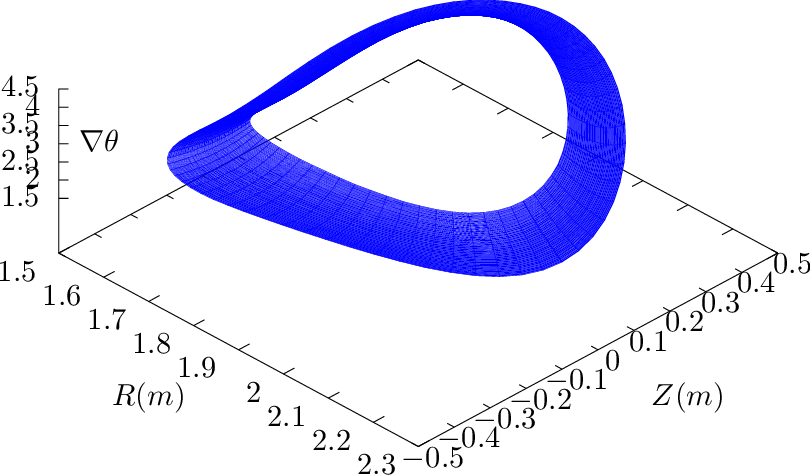
\includegraphics{/home/yj/theory/figures/pade/p.eps}
  \caption{\label{18-9-23-e1}Comparison between the exact value of $\Gamma_0 =
  \exp (- (k_{\perp} \rho)^2) I_0 ((k_{\perp} \rho)^2)$ and the corresponding
  Pade approximation $1 / (1 + (k_{\perp} \rho)^2)$.}
\end{figure}

Using the Pade approximation (\ref{18-10-23-p1}), the polarization density
$n_p$ in expression (\ref{18-9-23-p1}) can be written as
\begin{eqnarray}
  n_p & \approx & - \frac{q n_0}{T} \int \delta \Phi_k \exp (i\mathbf{k} \cdot
  \mathbf{x}) \frac{k_{\perp}^2 \rho^2}{1 + k_{\perp}^2 \rho^2}
  \frac{d\mathbf{k}}{(2 \pi)^3} .  \label{19-1-23-p6}
\end{eqnarray}
(Pad{\'e} approximate is the ``best'' approximation of a function by a
rational function of given order -- under this technique, the approximant's
power series agrees with the power series of the function it is
approximating.)

\subsubsection{Long wavelength approximation of the polarization density}

In the long wavelength limit, $k_{\perp} \rho \ll 1$, expression
(\ref{19-1-23-p6}) can be further approximated as
\begin{eqnarray}
  n_p & \approx & - \frac{q n_0}{T} \int \delta \Phi_k \exp (i\mathbf{k} \cdot
  \mathbf{x}) k_{\perp}^2 \rho^2 \frac{d\mathbf{k}}{(2 \pi)^3}, \nonumber\\
  & = & \frac{q n_0}{T} \rho^2 \nabla_{\perp}^2 \delta \Phi . 
  \label{19-1-23-p5}
\end{eqnarray}
Then the corresponding term in the Poisson equation is written as
\begin{eqnarray}
  \frac{q}{\varepsilon_0} n_p & = & \frac{q^2 n_0}{\varepsilon_0 T} \rho^2
  \nabla_{\perp}^2 \delta \Phi \nonumber\\
  & = & \frac{\rho^2}{\lambda_D^2} \nabla_{\perp}^2 \delta \Phi, 
  \label{18-9-23-p5}
\end{eqnarray}
where $\lambda_D$ is the Debye length defined by $\lambda_D^2 = T
\varepsilon_0 / (n_0 q^2)$. For typical tokamak plasmas, the thermal ion
gyroradius $\rho_i$ is much larger than $\lambda_D$. Therefore the term in
expression (\ref{18-9-23-p5}) for ions is much larger than the space charge
term $\nabla^2 \delta \Phi \equiv \nabla^2_{\perp} \delta \Phi +
\nabla^2_{\parallel} \delta \Phi \approx \nabla^2_{\perp} \delta \Phi$ in the
Poisson equation. Therefore the space charge term can be neglected in the long
wavelength limit.

Equation (\ref{18-9-23-p5}) also shows that electron polarization density is
smaller than the ion polarization density by a factor of $\rho_e / \rho_i
\approx 1 / 60$. Note that this conclusion is drawn in the long wavelength
limit. For short wavelength, the electron polarization and ion polarization
density can be of similar magnitude (to be discussed later).

\subsubsection{Polarization density expressed in terms of Laplacian operator}

The polarization density expression (\ref{19-1-23-p5}) is for the long
wavelength limit, which partially neglects FLR effect. Let us go back to the
more general expression (\ref{19-1-23-p6}). The Poisson equation is written
\begin{equation}
  - \varepsilon_0 \nabla_{\perp}^2 \delta \Phi = q_i \delta n_i + q_e \delta
  n_e .
\end{equation}
Write $\delta n_i = n_{p i} + \delta n_i'$, where $\delta n_{p i}$ is the ion
polarization density, then the above expression is written
\begin{equation}
  - \varepsilon_0 \nabla_{\perp}^2 \delta \Phi - q_i n_{p i} = q_i \delta n_i'
  + q_e \delta n_e .
\end{equation}
Fourier transforming in space, the above equation is written
\begin{equation}
  \label{19-1-23-p8} - \varepsilon_0 k_{\perp}^2 \delta \hat{\Phi} - q_i
  \hat{n}_{p i} = q_i \delta \hat{n}_i' + q_e \delta \hat{n}_e,
\end{equation}
where $\hat{n}_{p i}$ is the Fourier transformation (in space) of the
polarization density $n_{p i}$ and similar meanings for $\delta \hat{\Phi}$,
$\delta \hat{n}_i'$, and $\delta \hat{n}_e$. Expression (\ref{19-1-23-p6})
implies that $\hat{n}_{p i}$ is given by
\begin{equation}
  \hat{n}_{p i} = - \frac{q_i n_{i 0}}{T_i} \delta \hat{\Phi}
  \frac{k_{\perp}^2 \rho^2_i}{1 + k_{\perp}^2 \rho^2_i} .
\end{equation}
Using this, equation (\ref{19-1-23-p8}) is written
\begin{equation}
  - \varepsilon_0 k_{\perp}^2 \delta \hat{\Phi} - q_i \left( - \frac{q_i n_{i
  0}}{T_i} \frac{k_{\perp}^2 \rho^2_i}{1 + k_{\perp}^2 \rho^2_i} \delta
  \hat{\Phi} \right) = q_i \delta \hat{n}_i' + q_e \delta \hat{n}_e,
\end{equation}
Multiplying both sides by $(1 + k_{\perp}^2 \rho_i^2) / \varepsilon_0$, the
above equation is written
\begin{equation}
  - (1 + k_{\perp}^2 \rho^2_i) k_{\perp}^2 \delta \hat{\Phi} -
  \frac{q_i}{\varepsilon_0} \left( - \frac{q_i n_{i 0}}{T_i} (k_{\perp}^2
  \rho^2_i) \delta \hat{\Phi} \right) = \frac{1}{\varepsilon_0} (1 +
  k_{\perp}^2 \rho^2_i) (q_i \delta \hat{n}_i' + q_e \delta \hat{n}_e) .
\end{equation}
Next, transforming the above equation back to the real space, we obtain
\begin{equation}
  - (1 - \rho_i^2 \nabla_{\perp}^2) \nabla_{\perp}^2 \delta \Phi -
  \frac{q_i}{\varepsilon_0} \left( \frac{q_i n_{i 0}}{T_i} \rho_i^2
  \nabla_{\perp}^2 \delta \Phi \right) = \frac{1}{\varepsilon_0} (1 - \rho_i^2
  \nabla_{\perp}^2) (q_i \delta n_i' + q_e \delta n_e) .
\end{equation}
Neglecting the Debye shielding term, the above equation is written
\begin{equation}
  - \left( \frac{\rho_i^2}{\lambda_{D i}^2} \nabla_{\perp}^2 \delta \Phi
  \right) = \frac{1}{\varepsilon_0} (1 - \rho_i^2 \nabla_{\perp}^2) (q_i
  \delta n_i' + q_e \delta n_e),
\end{equation}
which is the equation actually solved in many gyrokinetic codes, where
$\lambda_{D i}^2 = \varepsilon_0 T_i / (q_i^2 n_{i 0})$.

\

\section{Polarization density matrix obtained by numerically integrating in
phase space using grid}

In Sec. \ref{21-8-22-a3}, to evaluate the polarization density, the potential
$\delta \Phi$ is Fourier expanded in space using local Cartesian coordinates,
and then the double gyro-angle integration of each harmonic is expressed as
the Bessel function. (It seems that the original motivation of using the
Fourier expansion here is to facilitate analytical treatment and is not
designed for numerical use. GEM code does make use of the local Fourier
expansion in its numerical implementation, where the local perpendicular wave
number needs to be estimated numerically, which seems awkward.)

In this section, we avoid using the local Fourier expansion, and directly
express the double gyro-angle integral as linear combination of values of
$\delta \Phi$ at spatial grid-points. The polarization density is given by Eq.
(\ref{18-9-13-p9}), i.e.,
\begin{equation}
  n_p (\mathbf{x}) = \frac{q}{m} \int d\mathbf{v} \left( (\delta \Phi -
  \langle \delta \Phi \rangle_{\alpha}) \frac{\partial F_0}{\partial
  \varepsilon} \right) .
\end{equation}
\begin{equation}
  n_p = M \delta \Phi
\end{equation}

\subsection{Direct evaluation of the double gyrophase integration}

Define
\begin{equation}
  A (\mathbf{x}) = - \frac{q}{m} \int d\mathbf{v} \left( \langle \delta \Phi
  \rangle_{\alpha} \frac{\partial F_0}{\partial \varepsilon} \right) .
\end{equation}
Using $d \mathbf{v} = v_{\perp} d v_{\perp} d v_{\parallel} d \alpha$, the
above integration is written as
\begin{equation}
  A (\mathbf{x}) = - \frac{q}{m} \int_{- \infty}^{\infty} d v_{\parallel}
  \int_0^{\infty} v_{\perp} d v_{\perp} \frac{\partial F_0}{\partial
  \varepsilon} \int_0^{2 \pi} d \alpha \langle \delta \Phi \rangle_{\alpha},
\end{equation}
where use has been made of the assumption that $\partial F_0 / \partial
\varepsilon$ is uniform in $\alpha$ in $(\mathbf{x}, v_{\perp}, v_{\parallel},
\alpha)$ coordinates, and thus is moved outside of the $\alpha$ integration.
Using the definition of gyro-averaging $(2 \pi)^{- 1} \int_0^{2 \pi} (\ldots)
d \alpha'$, the above integration is written as
\begin{equation}
  \label{21-8-22-e1} A (\mathbf{x}) = - \frac{q}{m} \int_{- \infty}^{\infty} d
  v_{\parallel} \int_0^{\infty} d v_{\perp} \frac{\partial F_{i 0}}{\partial
  \varepsilon} v_{\perp} \tmcolor{blue}{\int_0^{2 \pi} d \alpha \left(
  \frac{1}{2 \pi} \int_0^{2 \pi} \delta \Phi d \alpha' \right)} .
\end{equation}
Note that the gyro-averaging is performed in the guiding-center space, i.e.,
performed by varying the gyroangle $\alpha'$ while keeping guiding-center
position $\mathbf{X}$, $v_{\perp}$, and $v_{\parallel}$ constant. Using the
definition of $\delta \Phi_g$ (i.e., its relation with $\delta \Phi$):
\begin{equation}
  \delta \Phi_g (\mathbf{X}, \alpha', v_{\perp}) = \delta \Phi (\mathbf{x}),
\end{equation}
where the particle location $\tmmathbf{x}$ is computed from the guiding-center
location by
\begin{equation}
  \mathbf{x}=\mathbf{X}+\tmmathbf{\rho} (\mathbf{x}, \mathbf{v}) \approx
  \mathbf{X}-\mathbf{v} \times \frac{\mathbf{e}_{\parallel}
  (\mathbf{X})}{\Omega (\mathbf{X})},
\end{equation}
then $A (\mathbf{x})$ is written as
\begin{eqnarray*}
  &  & A (\mathbf{x})\\
  &  & = - \frac{q}{m} \int_{- \infty}^{\infty} d v_{\parallel}
  \int_0^{\infty} d v_{\perp} \frac{\partial F_{i 0}}{\partial \varepsilon}
  v_{\perp} \tmcolor{blue}{\int_0^{2 \pi} d \alpha \left[ \frac{1}{2 \pi}
  \int_0^{2 \pi} \delta \Phi \left( \mathbf{X}-\mathbf{v}_{\perp} (v_{\perp},
  \alpha') \times \frac{\mathbf{e}_{\parallel} (\mathbf{X})}{\Omega
  (\mathbf{X})} \right) d \alpha' \right]}\\
  &  & \approx - \frac{q}{m} \int_{- \infty}^{\infty} d v_{\parallel}
  \int_0^{\infty} d v_{\perp} \frac{\partial F_{i 0}}{\partial \varepsilon}
  v_{\perp} \tmcolor{blue}{\int_0^{2 \pi} d \alpha \left[ \frac{1}{N_2}
  \sum_{j = 1}^{N_2} \delta \Phi \left( \mathbf{X}-\mathbf{v}_{\perp}
  (v_{\perp}, \alpha'_j) \times \frac{\mathbf{e}_{\parallel}
  (\mathbf{X})}{\Omega (\mathbf{X})} \right) \right]}
\end{eqnarray*}
where $\mathbf{v}_{\perp} = \mathbf{v} (v_{\perp}, \alpha_j')$ denotes a
perpendicular velocity corresponding to a discrete gyro-angle $\alpha_j'$.

Next, in order to perform the remaining velocity space integration, transform
back to the particle coordinates (because the velocity integration is
performed in the particle coordinates, i.e., it is performed by keeping the
particle coordinate $\mathbf{x}$ constant):
\begin{eqnarray}
  &  & A (\mathbf{x}) = - \frac{q}{m} \int_{- \infty}^{\infty} d
  v_{\parallel} \int_0^{\infty} d v_{\perp} \frac{\partial F_{i 0}}{\partial
  \varepsilon} v_{\perp} \nonumber\\
  &  & \times \tmcolor{blue}{\int_0^{2 \pi} d \alpha \left[ \frac{1}{N_2}
  \sum_{j = 1}^{N_2} \delta \Phi \left( \mathbf{x} +\mathbf{v}_{\perp}
  (v_{\perp}, \alpha) \times \frac{\mathbf{e}_{\parallel} (\mathbf{X})}{\Omega
  (\mathbf{X})} -\mathbf{v}_{\perp} (v_{\perp}, \alpha_j') \times
  \frac{\mathbf{e}_{\parallel} (\mathbf{X})}{\Omega (\mathbf{X})} \right)
  \right]} \nonumber\\
  &  & \approx - \frac{q}{m} \int_{- \infty}^{\infty} d v_{\parallel}
  \int_0^{\infty} d v_{\perp} \frac{\partial F_{i 0}}{\partial \varepsilon}
  v_{\perp} \nonumber\\
  &  & \times \tmcolor{blue}{\int_0^{2 \pi} d \alpha \left[ \frac{1}{N_2}
  \sum_{j = 1}^{N_2} \delta \Phi \left( \mathbf{x} +\mathbf{v}_{\perp}
  (v_{\perp}, \alpha) \times \frac{\mathbf{e}_{\parallel} (\mathbf{x})}{\Omega
  (\mathbf{x})} -\mathbf{v}_{\perp} (v_{\perp}, \alpha_j') \times
  \frac{\mathbf{e}_{\parallel} (\mathbf{x})}{\Omega (\mathbf{x})} \right)
  \right]} \nonumber\\
  &  & \approx - \frac{q}{m}  \int_{- \infty}^{\infty} d v_{\parallel}
  \int_0^{\infty} d v_{\perp} \frac{\partial F_{i 0}}{\partial \varepsilon}
  v_{\perp} \nonumber\\
  &  & \times \tmcolor{blue}{\frac{2 \pi}{N_1} \sum_{i = 1}^{N_1}
  \frac{1}{N_2}  \sum_{j = 1}^{N_2} \delta \Phi \left( \mathbf{x}
  +\mathbf{v}_{\perp} (v_{\perp}, \alpha_i) \times
  \frac{\mathbf{e}_{\parallel} (\mathbf{x})}{\Omega (\mathbf{x})}
  -\mathbf{v}_{\perp} (v_{\perp}, \alpha_j') \times
  \frac{\mathbf{e}_{\parallel} (\mathbf{x})}{\Omega (\mathbf{x})} \right) .} 
  \label{21-9-16-a4}
\end{eqnarray}
For notation ease, define
\begin{equation}
  \Delta \mathbf{\rho}_{i j} =\mathbf{v}_{\perp} (v_{\perp}, \alpha_i) \times
  \frac{\mathbf{e}_{\parallel} (\mathbf{x})}{\Omega (\mathbf{x})}
  -\mathbf{v}_{\perp} (v_{\perp}, \alpha_j') \times
  \frac{\mathbf{e}_{\parallel} (\mathbf{x})}{\Omega (\mathbf{x})},
\end{equation}
where $\Delta \mathbf{\rho}_{i j}$ is a function of $(\mathbf{x}, v_{\perp},
\alpha_i, \alpha_j')$. Then Eq. (\ref{21-9-16-a4}) is written as
\begin{eqnarray}
  A (\mathbf{x}) & = & - \frac{q}{m}  \int_{- \infty}^{\infty} d v_{\parallel}
  \int_0^{\infty} d v_{\perp} \frac{\partial F_{i 0}}{\partial \varepsilon}
  v_{\perp} \tmcolor{blue}{\frac{2 \pi}{N_1} \sum_{i = 1}^{N_1} \frac{1}{N_2} 
  \sum_{j = 1}^{N_2} \delta \Phi (\mathbf{x} + \Delta \mathbf{\rho}_{i j})} . 
  \label{22-11-8-1}
\end{eqnarray}
The guiding-center transform and its inverse involved in the above are
illustrated in Fig. \ref{21-8-22-a1}, which also shows how to evaluate the
double gyro-angle integration using the discrete values of $\delta \Phi_{i
j}$.

\

\begin{figure}[h]
  \resizebox{238pt}{237pt}{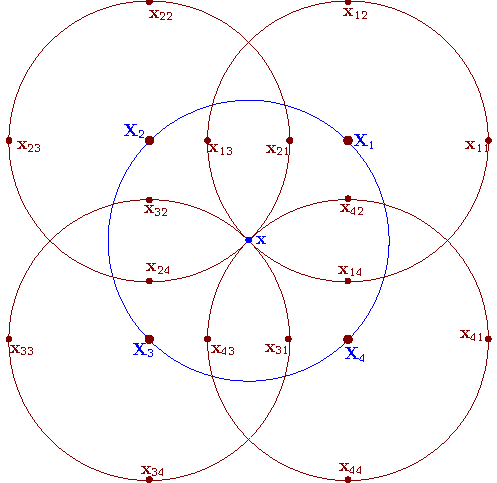
\includegraphics{nonlinear_gyrokinetic_equation-1.pdf}}
  \caption{\label{21-8-22-a1}Given a $v_{\perp}$, then the double gyro-angle
  integration in Eq. (\ref{21-8-22-e1}) at a particle location $\mathbf{x}$ is
  evaluated by the following steps: Use the guiding center transform to get
  guiding-center locations (four locations are shown in this case, namely
  $\mathbf{X}_i$ with $i = 1, 2, 3, 4$, corresponding gyro-angle $\alpha_i$
  with $i = 1, 2, 3, 4$; 2.) For each guiding-center location, use the inverse
  guiding-center transform to calculate points on the corresponding gyro-ring
  (four points are shown for each guiding-center $\mathbf{X}_i$ in this case,
  namely $\mathbf{x}_{i j}$ with $j = 1, 2, 3, 4$, corresponding gyro angle
  $\alpha_j'$ with $j = 1, 2, 3, 4$.) Then the double gyro-angle integral
  appearing in the polarization density is approximated as
  $\label{21-9-2-a1} \int_0^{2 \pi} d \alpha \left( \int_0^{2 \pi} \delta \Phi
  (\mathbf{x}) d \alpha' \right) \approx \frac{(2 \pi)^2}{N_1 N_2}  \sum_{i =
  1}^{N_1} \sum_{j = 1}^{N_2} \delta \Phi (\mathbf{x}_{i j}),$
  where $N_1 = 4, N_2 = 4$ for the case shown here.}
\end{figure}

The spatial points $\mathbf{x}_{i j}$ appearing in Eq. (\ref{21-9-2-a1}) are
not necessarily grid points. Linear interpolations are used to express $\delta
\Phi (\mathbf{x}_{i j})$ as linear combination of values of $\delta \Phi$ at
grid-points.

\subsection{Performing the parallel velocity integration}

Assume that $F_0$ is Maxwellian, then
\begin{equation}
  \frac{\partial F_0}{\partial \varepsilon} = - \frac{m}{T} f_M = -
  \frac{m}{T} \frac{n_0}{(2 \pi T / m)^{3 / 2}} \exp \left( \frac{- m
  v^2_{\parallel}}{2 T} \right) \exp \left( \frac{- m v^2_{\perp}}{2 T}
  \right) .
\end{equation}
Note that $\Delta \mathbf{\rho}_{i j}$ is independent of $v_{\parallel}$. Then
the integration over $v_{\parallel}$ in Eq. (\ref{22-11-8-1}) can be
analytically performed, yielding


\begin{eqnarray}
  A (\mathbf{x}) & = & \frac{q}{T}  \int_{- \infty}^{\infty} d
  \overline{v}_{\parallel} \exp \left( \frac{- \overline{v}^2_{\parallel}}{2}
  \right) \int_0^{\infty} d \overline{v}_{\perp} \overline{v}_{\perp}
  \frac{n_0}{(2 \pi)^{3 / 2}} \exp \left( \frac{- \overline{v}^2_{\perp}}{2}
  \right) \nonumber\\
  & \times & \frac{2 \pi}{N_1} \sum_{i = 1}^{N_1} \frac{1}{N_2}  \sum_{j =
  1}^{N_2} \delta \Phi (\mathbf{x} + \Delta \mathbf{\rho}_{i j}) \nonumber\\
  & = & n_0  \int_0^{\infty} d \overline{v}_{\perp} \overline{v}_{\perp} \exp
  \left( \frac{- \overline{v}^2_{\perp}}{2} \right) \frac{1}{N_1} \sum_{i =
  1}^{N_1} \frac{1}{N_2}  \sum_{j = 1}^{N_2} \frac{q}{T} \delta \Phi
  (\mathbf{x} + \Delta \mathbf{\rho}_{i j}) .  \label{21-9-16-a5}
\end{eqnarray}
where $\overline{v}_{\parallel} = v_{\parallel} / v_t$, $\overline{v}_{\perp}
= v_{\perp} / v_t$, \ $v_t = \sqrt{T / m}$, and use has been made of
\begin{equation}
  \int_{- \infty}^{\infty} \exp \left( - \frac{x^2}{2} \right) d x = \sqrt{2
  \pi} .
\end{equation}

\subsection{Toroidal Fourier transform of polarization density in
field-aligned coordinates}

In field-aligned coordinates $(x, y, z)$, Fourier expansion of $\delta \Phi$
along $y$ is written
\begin{equation}
  \delta \Phi (\mathbf{x}) = \sum_{n = - N_t}^{N_t} \exp \left( \iota n
  \frac{2 \pi}{L_y} y \right) \delta \Phi_n (x, z),
\end{equation}
where $\iota = \sqrt{- 1}$, $N_t$ is the number of toroidal harmonics
included. Use this in Eq. (\ref{21-9-16-a5}), yielding
\begin{eqnarray}
  A (\mathbf{x}) & = & n_0  \int_0^{\infty} d \overline{v}_{\perp}
  \overline{v}_{\perp} \exp \left( \frac{- \overline{v}^2_{\perp}}{2} \right)
  \nonumber\\
  & \times & \frac{1}{N_1} \sum_{i = 1}^{N_1} \frac{1}{N_2}  \sum_{j =
  1}^{N_2} \left[ \frac{q}{T}  \sum_{n = - N_t}^{N_t} \exp \left( \iota n
  \frac{2 \pi}{L_y} (y + \Delta \rho_{i j y}) \right) \delta \Phi_n (x +
  \Delta \rho_{i j x}, z + \Delta \rho_{i j z}) \right] \nonumber\\
  & = & n_0  \sum_{n = - N_t}^{N_t} \exp \left( \iota n \frac{2 \pi}{L_y} y
  \right) \int_0^{\infty} d \overline{v}_{\perp} \overline{v}_{\perp} \exp
  \left( \frac{- \overline{v}^2_{\perp}}{2} \right) \nonumber\\
  & \times & \frac{1}{N_1} \sum_{i = 1}^{N_1} \frac{1}{N_2}  \sum_{j =
  1}^{N_2} \left[ \exp \left( \iota n \frac{2 \pi}{L_y} \Delta \rho_{i j y}
  \right) \frac{q}{T} \delta \Phi_n (x + \Delta \rho_{i j x}, z + \Delta
  \rho_{i j z}) \right] .  \label{21-9-16-a1}
\end{eqnarray}
From Eq. (\ref{21-9-16-a1}), the Fourier expansion coefficient of $A
(\mathbf{x})$ in $y$ can be identified, which is
\begin{eqnarray}
  A_n (x, z) & = & n_0  \int_0^{\infty} d \overline{v}_{\perp}
  \overline{v}_{\perp} \exp \left( \frac{- \overline{v}^2_{\perp}}{2} \right)
  \nonumber\\
  & \times & \frac{1}{N_1} \sum_{i = 1}^{N_1} \frac{1}{N_2}  \sum_{j =
  1}^{N_2} \left[ \exp \left( \iota n \frac{2 \pi}{L_y} \Delta \rho_{i j y}
  \right) \frac{q}{T} \delta \Phi_n (x + \Delta \rho_{i j x}, z + \Delta
  \rho_{i j z}) \right] .  \label{22-12-21-1}
\end{eqnarray}
Let us make the following approximation
\begin{equation}
  \label{22-12-21-3} \delta \Phi_n (x + \Delta \rho_{i j x}, z + \Delta
  \rho_{i j z}) \approx \delta \Phi_n (x + \Delta \rho_{i j x}, z),
\end{equation}
which should be a good approximation since the variation of $\delta \Phi$
along a field line over a distance of a Larmor radius is small. Then
expression (\ref{22-12-21-1}) is written as
\begin{eqnarray}
  &  & A_n (x, z) \approx n_0  \int_0^{\infty} d \overline{v}_{\perp}
  \overline{v}_{\perp} \exp \left( \frac{- \overline{v}^2_{\perp}}{2} \right)
  \nonumber\\
  &  & \times \frac{1}{N_1} \sum_{i = 1}^{N_1} \frac{1}{N_2}  \sum_{j =
  1}^{N_2} \left[ \exp \left( \iota n \frac{2 \pi}{L_y} \Delta \rho_{i j y}
  \right) \frac{q}{T} \delta \Phi_n (x + \Delta \rho_{i j x}, z) \right] . 
\end{eqnarray}
The approximation (\ref{22-12-21-3}) makes the operator $A_n$ on $\delta
\Phi_n$ become local in $z$ direction, i.e., it involves the value of $\delta
\Phi_n$ at a single location $z$. This makes $A_n (x, z)$ reduce to a 1D
operator on $\delta \Phi_n$ in the $x$ direction.

\subsection{Using MC integration, to be continued, not necessary}

The integration we try to express is given by
\begin{eqnarray}
  A_{i j k} & \approx & \frac{1}{V_{i j k}} \int_{V_{i j k}} d\mathbf{x}n_p
  (\mathbf{x}) \nonumber\\
  & = & \frac{1}{V_{i j k}} \int_{V_{i j k}} d\mathbf{x} \int d\mathbf{v}
  \left( \frac{q}{m} (\delta \Phi - \langle \delta \Phi \rangle_{\alpha})
  \frac{\partial F_0}{\partial \varepsilon} \right), 
\end{eqnarray}
where $A_{i j k}$ is the value of $n_p (\mathbf{x})$ at a grid-point, which is
approximated by the spatial averaging of $n_p (\mathbf{x})$ over the cell
whose center is the grid-point, $V_{i j k}$ is the volume of the cell. We will
use Monte-Carlo guiding-center markers to compute the above cell average.
\begin{eqnarray*}
  A_{i j k}^{(1)} & = & - \frac{q}{m} \frac{1}{V_{i j k}} \sum_p \sum_{\alpha}
  \left( \langle \delta \Phi \rangle_{\alpha} \frac{\partial F_0}{\partial
  \varepsilon} \frac{1}{g} \right)\\
  & = & - \frac{q}{m} \frac{1}{V_{i j k} } \sum_p \langle \delta \Phi
  \rangle_{\alpha} \sum_{\alpha} \left( \frac{\partial F_0}{\partial
  \varepsilon} \frac{1}{g} \right)
\end{eqnarray*}
Nearest neighbour interpolation


\begin{eqnarray*}
  A_{i j k}^{(2)} & = & - \frac{q}{m} \frac{1}{V_{i j k}} \sum_p \sum_{\alpha}
  \left( \delta \Phi \frac{\partial F_0}{\partial \varepsilon} \frac{1}{g}
  \right)\\
  & = & - \frac{q}{m} \frac{\delta \Phi_{i j k}}{V_{i j k}} \sum_p
  \sum_{\alpha} \left( \frac{\partial F_0}{\partial \varepsilon} \frac{1}{g}
  \right)
\end{eqnarray*}
Later, I found that evaluating the polarization density using grid work well.
Therefore there is no need to evaluate it using MC markers, which is more
complicated.

\

\

\appendix\section{Implementation of gyrokinetics in particle-in-cell (PIC)
codes}

\subsection{Monte-Carlo evaluation of distribution function moment at
grid-points}

Suppose that the 6D guiding-center phase-space $(\mathbf{X}, \mathbf{v})$ is
described by $(\psi, \theta, \phi, v_{\parallel}, \alpha, v_{\perp})$
coordinates. The Jacobian of the coordinate system is given by $\mathcal{J} =
\mathcal{J}_r v_{\perp} \mathcal{}$, where $\mathcal{J}_r = \mathcal{J} (\psi,
\theta)$ is the Jacobian of the coordinates $(\psi, \theta, \phi)$.

Suppose that we sample the 6D phase-space by using a probability function $P
(\psi, \theta, \phi, v_{\perp}, \alpha, v_{\parallel})$. (Then the effecitive
probability function used in rejection method is $P \mathcal{J}_r
v_{\perp}$.). We will sample a distribution function $\delta f_g (\mathbf{X},
v_{\perp}, v_{\parallel}, \alpha)$ that happens to be independent of the
gyro-angle $\alpha$ using the above markers.

Since there is no indication that some values of $\alpha$ would be more
important than others, it is natural to smaple $\alpha$ using a uniform
probability function, i.e., $P (\mathbf{X}, v_{\perp}, \alpha, v_{\parallel})$
can be chosen to be independent of $\alpha$.

In terms of sampling $\delta f_g (\mathbf{X}, v_{\perp}, \alpha,
v_{\parallel})$, there is no need to specify $\alpha$ because both $f_g$ and
marker distribution $g = N_p P$ are indepedent of $\alpha$, and thus the
weight $\delta f_g / g$ is also independent of $\alpha$. It turns out that
sampling $\alpha$ is necessary in simulations. The reason is as follows. The
density needed in solving the field equation is the moement of the particle
distribution function $\delta f_p (\mathbf{x}, v_{_{\perp}}', \alpha',
v_{\parallel}')$ at fixed $\mathbf{x}$, and $\delta f_p (\mathbf{x},
v_{_{\perp}}', \alpha', v_{\parallel}')$ is not uniform in $\alpha'$. [Proof:
$\delta f_p (\mathbf{x}, v_{_{\perp}}', \alpha', v_{\parallel}')$ with only
$\alpha'$ changing corresponds to both $\mathbf{X}$ and $\alpha$ changing in
$(\mathbf{X}, v_{\perp}, \alpha, v_{\parallel})$ coordinates, and thus the
corresponding $\delta f_g (\mathbf{X}, v_{\perp}, \alpha, v_{\parallel})$,
which is equal to $\delta f_p (\mathbf{x}, v_{_{\perp}}', \alpha',
v_{\parallel}')$, is varying because $\delta f_g$ is dependent on $\mathbf{X}$
and is independent of $\alpha$.] Therefore $\alpha'$ needs to be specified in
$(\mathbf{x}, v_{_{\perp}}', \alpha', v_{\parallel}')$ coordinates, which can
be achieved by specifying $\alpha$ in $(\mathbf{X}, v_{\perp}, \alpha,
v_{\parallel})$ because of $\alpha' = \alpha$.

\

From the perspective of programming, it is ready to understand why $\alpha$
needs to be specified. When computing density at grid-points, we need to
compute particle locations from the guiding-center locations which requires us
to specify the gyro-angle $\alpha$ for each marker.

Markers in guiding-center space $(\mathbf{X}, v_{\perp}, \alpha,
v_{\parallel})$ with fixed $(\mathbf{X}, v_{\perp}, v_{\parallel})$ but
varying $\alpha$ correspond to markers in particle space with varying
locations and varying $\alpha'$ (marker weights are constant since marker
weights in guiding-center space with only $\alpha$ varying are constant). In
the PIC method of computing the particle density at fixed $\mathbf{x}$, the
contribution of each particle marker to the density is solely determined by
the distance of the particle marker to the fixed $\mathbf{x}$ (the gyro-angle
$\alpha'$ has not effect here). Therefore different values of $\alpha$
contributes differently to the density, and thus the resolution of $\alpha$
matters.

For a marker with coordinators $(\mathbf{X}, v_{\perp}, v_{\parallel},
\alpha)$, where $\alpha$ is the gyro-angle, the corresponding particle
position can be calculated by using the inverse guiding-center transformation
(\ref{19-1-19-p2}). Then we can deposit the marker weight to grid-points in
the same way that we do in conventional PIC simulations. Looping over all
markers, we build the particle density at grids.

Compared with conventional PIC methods, where particle positions are directly
sampled, what is the benefit of sampling guiding-center positions and then
transform them back to the particle positions? More computations are involved
since we need to numerically perform the inverse guiding-center
transformation. The answer lies in the important fact that the distribution
function $f_g (\mathbf{X}, v_{\perp}, v_{\parallel}, \alpha)$ that needs to be
numerically evolved in gyrokinetic simulation is actually independent of the
gyro-angle $\alpha$. Furthermore, we use a probability density function $P$
that is independent of $\alpha$ to sample the 6D phase space $(\mathbf{X},
v_{\perp}, v_{\parallel}, \alpha)$. Then the marker weight $w \equiv f_g /
(N_p P)$ is independent of $\alpha$, where $N_p$ is number of markers loaded.

Suppose we have a concrete sampling of $f_g$ in the 6D phase-space
$(\mathbf{X}, v_{\perp}, v_{\parallel}, \alpha)$, i.e., $(\mathbf{X}_j,
v_{\perp j}, v_{\parallel j}, \alpha_j, w_j)$ with $j = 1, \ldots, N_p$, then
we can do the inverse guiding-center transform and then deposit particles to
the grids to obtain a moment (e.g. density).

Since $P \mathcal{J}_{r v}$, where $\mathcal{J}_{r v} = \mathcal{J}_r
v_{\perp}$ is the Jacobian of $(\mathbf{X}, v_{\perp}, v_{\parallel},
\alpha)$, is independent of $\alpha$, the sampling $\alpha_j$ with $j = 0, 1,
\ldots, N_p$ are uniform distributed random numbers. Therefore we can generate
another sampling of $\alpha$ (denoted by $\alpha_j'$ with $j = 1, \ldots,
N_p$) using random number generators and combine $\alpha_j'$ with the old
sampling $(\mathbf{X}_j, v_{\perp j}, v_{\parallel j})$ to obtain a new
sampling $(\mathbf{X}_j, v_{\perp j}, v_{\parallel j}, \alpha_j', w_j')$. \
The values of $w$ at the new sampling points are equal to the original values,
i.e., $w_j' = w_j$ since the particle weight $w = f_g / (N_p P)$ is
independent of $\alpha$. \ Using the new sampling and following the same
procedures given above, we can estimate values of the moment at grid-points
again, which will differ from the estimation obtained using the old sampling.
Taking the average of the two estimations will give a more accurate estimation
because the resolution in the gyro-angle is increased.

[Note that even if $P \mathcal{J}_{r v}$ is dependent on $\alpha$ due to the
possible dependence of $\mathcal{J}_{r v}$ on $\alpha$, we still can easily
generate a new set of sampling which differs from the old sampling only in
$\alpha$. Specifically, in the rejection method, we use the old sampling
$(\mathbf{X}_j, v_{\perp j}, v_{\parallel j})$ for each reject step and only
adjust $\alpha$ to satisfy the acceptance criteria.]

We can also construct a new sampling by replacing $\alpha_j$ by $\alpha_j +
\Delta$, where $\Delta$ is a constant. Then the new sampling is given by
$(\mathbf{X}_j, v_{\perp j}, v_{\parallel j}, \alpha_j + \Delta, w_j')$ with
$j = 1, \ldots, N_p$. Since the original sampling probability function $P
\mathcal{J}_r v_{\perp}$ is independent of $\alpha$, then $(\mathbf{X}_j,
v_{\perp j}, v_{\parallel j}, \alpha_j + \Delta)$ is still a consistent
sampling that can be generated by the original probability function $P
\mathcal{J}_r v_{\perp}$. Furthermore, since the particle weight $w = f_g /
(N_p P)$ is independent of $\alpha$, we infer that the values of $w$ at the
new sampling points are equal to the original values, i.e., $w_j' = w_j$.

In doing the deposition, each marker has a single gyro-angle. Due to the
independence of the weight $(w = f_g / (N_p P))$ of the gyro-angle, the
resolution over the gyro-angle can be increased in a way that there can be
several gyro-angles for a single $(\mathbf{X}_j, v_{\perp j}, v_{\parallel
j})$. This gives the wrong impression that the gyro-angle of a guiding-center
marker is arbitrary. The correct understanding is that given above, i.e., we
do 4 separate sampling of the phase space and then average the results.

In the code, the gyro-angle is defined relative to the direction $\nabla \psi
/ | \nabla \psi |$ at the guiding-center position. Specifically, the
gyro-angle is defined as the included angle between $\nabla \psi / | \nabla
\psi |$ and $-\mathbf{v} \times \mathbf{e}_{\parallel} (\mathbf{x}) / \Omega
(\mathbf{x})$, where $\mathbf{e}_{\parallel} (\mathbf{x}) / \Omega
(\mathbf{x})$ is approximated by the value at the guiding-center location.

\

Then $(\mathbf{X}_j, v_{\perp j}, v_{\parallel j})$ can be evolved by using
the guiding-center motion equation. (It is obvious how to evalute the
gyro-averaging of the electromagnetic fields needed in pusing markers.)


\begin{equation}
  \Phi (\mathbf{x}) = \sum_{i, j} \Phi_{i j} c_{i j} (\mathbf{x}) .
\end{equation}
\subsection{Monte-Carlo sampling of 6D guiding-center phase-space
}\label{19-1-28-1}

Suppose that the 6D guiding-center phase-space $(\mathbf{X}, \mathbf{v})$ is
described by $(\psi, \theta, \phi, v_{\parallel}, v_{\perp}, \alpha)$
coordinates. The Jacobian of the coordinate system is given by $\mathcal{J} =
\mathcal{J}_r v_{\perp} \mathcal{}$, where $\mathcal{J}_r = \mathcal{J} (\psi,
\theta)$ is the Jacobian of the coordinates $(\psi, \theta, \phi)$. Suppose
that we sample the 6D phase-space by using the following probability density
function:
\begin{equation}
  \label{19-1-26-1} P (\psi, \theta, \phi, v_{\parallel}, v_{\perp}, \alpha) =
  \frac{1}{V_r} \left( \frac{m}{2 \pi T} \right)^{3 / 2} \exp \left[ - \frac{m
  (v_{\parallel}^2 + v_{\perp}^2)}{2 T} \right],
\end{equation}
where $V_r$ is the volume of the spatial simulation box, $T$ is a constant
temperature. $P$ given above is independent of $\psi, \theta, \phi$ and
$\alpha$. It is ready to verify that the above $P$ satisfies the following
normalization condition:
\begin{equation}
  \int_{V_r} \int P d\mathbf{v}d\mathbf{X}= \int_{V_r} \int_{- \infty}^{+
  \infty} \int_0^{\infty} \int_0^{2 \pi} P v_{\perp} d \alpha d v_{\perp} d
  v_{\parallel} \mathcal{J}_r d \psi d \theta d \phi = 1.
\end{equation}
I use the rejection method to numerically generate $N_p$ markers that satisfy
the above probability density function. [The effective probability density
function actually used in the rejection method is $P'$, which is related to
$P$ by
\begin{equation}
  P' = | \mathcal{J}_r \mathcal{J}_v | P = | \mathcal{J}_r (\psi, \theta) |
  v_{\perp} P
\end{equation}
Note that $P'$ does not depend on the gyro-angle $\alpha$.]

Then the weight of a marker is written
\begin{equation}
  w = \frac{\delta f_g (\psi, \theta, \phi, v_{\parallel}, v_{\perp})}{N_p P}
  .
\end{equation}
Since both $f_g$ and $P$ is independent of the gyro-angle $\alpha$, $w$ is
also independent of $\alpha$.

The numerical representation of $\delta f_g$ is written
\begin{equation}
  \delta \tilde{f}_g = \frac{1}{\mathcal{J}_r v_{\perp}} \sum_j^{N_p} w_j
  \delta (\psi - \psi_j) \delta (\theta - \theta_j) \delta (\phi - \phi_j)
  \delta (v_{\parallel} - v_{\parallel j}) \delta (v_{\perp} - v_{\perp j})
  \delta (\alpha - \alpha_j) .
\end{equation}
Although the distribution function $\delta f_g$ to be sampled is independent
of the gyro-angle $\alpha$, we still need to specify the gyro-angle because we
need to use the inverse guiding-center transformation, which needs the
gyro-angle. Each marker needs to have a specific gyro-angle value $\alpha_j$
so that we know how to transform its $\mathbf{X}_j$ to $\mathbf{x}_j$ and then
do the charge deposition in $\mathbf{x}$ space.

To increase the resolution over the gyro-angle (the quantity of intest to us,
e.g., density, is the integration of the particle distribution function at
fixed spatial location, and the distribution at the fixed location is not
uniform in the gyro-angle), we need to load more markers. However, thanks to
the fact that both sampling probability density function $P$ and $\delta f_g$
are independent of $\alpha$, the resolution over the gyro-angle can be
increased in a simple way.
\begin{equation}
  n (\mathbf{x}) = \frac{n_1 (\mathbf{x}) + n_2 (\mathbf{x}) + n_3
  (\mathbf{x}) + n_4 (\mathbf{x})}{4} .
\end{equation}
This corresponds to sampling the 6D phase-space 4 separate times (each time
with identical sampling points in $(\mathbf{X}, v_{\parallel}, v_{\perp})$ but
different sampling points in $\alpha$) and then using the averaging of the 4
Monte-Carlo integrals to estimate the exact value. This estimation can also be
(roughly) considered as a Monte-Carlo estimation using 4 times larger number
of markers as that is originally used (the Monte-Carlo estimation using truly
4 time larger number of markers is more accurate than the result we obtained
above because the former also increase the resolution of $(\mathbf{X},
v_{\parallel}, v_{\perp})$ while the latter keeps the resolution of
$(\mathbf{X}, v_{\parallel}, v_{\perp})$ unchanged.)

In numerical code, we choose $N$ sampling points that are evenly distributed
on the gyro-ring ($N$ is usually $4$ as a compromise between efficiency and
accuracy). Denote the Mote-Carlo weight of the $j \tmop{th}$ marker by $w_j$.
Then the weight is evenly split by the $N$ sub-markers on the gyro-ring.
Therefore each sub-marker have a Monte-Carlo weight $w_j / N$. Then
calculating the integration (\ref{19-1-19-p1}) at a grid corresponds to
depositing all the $N$ sub-markers associated with each guiding-center marker
to the grid, as is illustrated in Fig. \ref{19-1-19-p4}. However, interpreting
in this way is confusing to me because, with a single sampling of the
phase-space, the phase-space volume or weight can not be easily split. I
prefer the above interpretation that the 6D phase space is sampled 4 separate
times and thus we get 4 estimations and finally we take the averaging of these
4 estimations. It took a long time for me to finally find this way of
understanding.

\begin{figure}[h]
  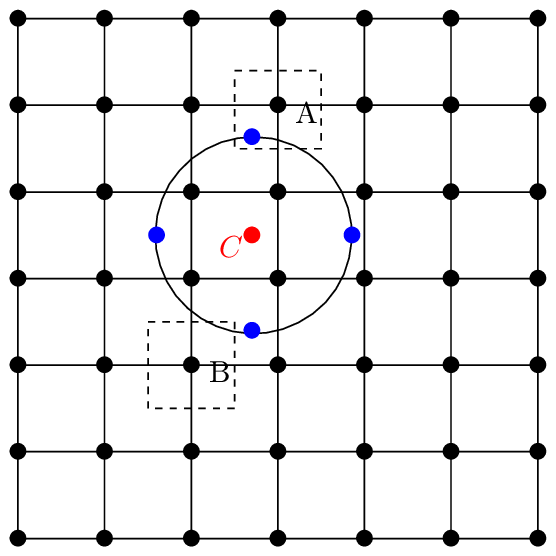
\includegraphics{/home/yj/theory/figures/grids_cells/grids-3.eps}
  \caption{\label{19-1-19-p4}The spatial grid in the plane perpendicular to
  the equilibrium magnetic field, a guiding-center marker \tmcolor{red}{$C$},
  and its gyro-ring with \tmcolor{blue}{4 sampling points} (sub-markers) on
  it. The 4 sub-markers are calculated by using the transformation
  (\ref{19-1-19-p2}) (inverse guiding-center transform). Assume that
  Monte-Carlo weight of the guiding-center marker \tmcolor{red}{$C$} is $w_j$.
  Then The Monte-Carlo weight of each sub-marker is $w_j / 4$. The value of
  integration (\ref{19-1-19-p1}) at a grid point is approximated by $I /
  \Delta V$, where $I$ is the Monte-Carlo integration of all sub-markers
  (associated with all guiding-center markers) in the cell, $\Delta V$ is the
  cell volume. The cell associated with a grid-point (e.g., $A$) is indicated
  by the dashed rectangle (this is for the 2D projection, the cell is 3D and
  it is a cube). If the Dirac delta function is used as the shape function of
  the sub-markers, then calculating the contribution of a sub-marker to a grid
  corresponds to the nearest-point interpolation (for example, the 4
  sub-markers will contribute nothing to grid point $B$ since no-sub marker is
  located within the cell). In practice, the flat-top shape function with its
  support equal to the cell size is often used, then the depositing
  corresponds to linearly interpolating the weight of each sub-marker to the
  nearby grids.}
\end{figure}

\

In summary, the phase-space to be sampled in gyrokinetic simulations are
still 6D rather than 5D. In this sense, the statement that gyrokinetic
simulation works in a 5D phase space is misleading. We are still working in
the 6D phase-space. The only subtle thing is that the sixth dimension, i.e.,
gyro-angle, can be sampled in an easy way that is independent of the other 5
variables.

In numerical implementation, the gyro-angle may not be explicitly used. We
just try to find 4 arbitrary points on the gyro-ring that are easy to
calculate. Some codes (e.g. ORB5) introduces a random variable to rotate these
4 points for different markers so that the gyro-angle can be sampled less
biased.

From the view of particle simulations, the gyrokinetic model can be
considered as a noise reduction method, where the averaging over the
gyro-angle is equivalent to a time averaging over a gyro-period, which reduces
the fluctuation level (in both time and space) associated with evaluating the
Monte-Carlo phase integration. Here the averaging in gyrokinetic particle
simulation refers to taking several points on a gyro-ring when depositing
markers to spatial grids to obtain the density and current on the grids.
(Another gyro-averaging appears in evaluating the guiding-center drift.) In
gyrokinetic particle simulation, even a step size smaller than a gyro-period
is taken, the quantities used in the model is still the ones averaged over one
gyro-period. In this sense, a gyrokinetic simulation is only meaningful when
the time step size is larger than one gyro-period. [**Some authors may
disagree with that the gyro-averaging is a time-averaging. They may consider
the gyro-averaging as the phase-space integration over the gyro-angle
coordinate. This view seems to be right in Euler simulations but seems to be
wrong in particle simulations. The reason is as follows. For each marker,
choose a random gyro-phase and then do the inverse transformation to obtain
particle position, and sum over all markers (this corresponds to phase-space
Monte-Carlo integration, which include the gyro-angle integration, so no
further gyro-angle integration is needed); choose another random gyro-phase
and repeat the above procedure (this can be interpreted as do the phase-space
Monte-Carlo integration at another time), choose further random gyro-phase for
each marker and repeat. Finally averaging all the above values to obtain the
final estimation of the phase-space integration. This amounts to a
time-averaging over a gyro-motion. In summary, sampling several times with
different gyro-phases for each marker and taking the average amounts to the
time averaging over gyro-motion**]

When doing the time-average over the ion cyclotron motion, the time variation
of the low-frequency mode is negligible and only the spatial variation of the
modes is important. For the gyro-motion, only the gyro-angle is changing and
all the other variables, $(\mathbf{X}, v_{\perp}, v_{\parallel})$, \ are
approximately constant. As a result, this time averaging finally reduces to a
gyro-averaging.

\

I am always reasoning in terms of particle position and velocity, considering
the guiding-center location as an image of the particle position. When working
in the guiding-center coordinates, I always reason by transforming back to the
particle position. This reasoning is clear and help me avoid some confusions I
used to have.

\

\

\subsection{Distribution function transform**check}

In the above, we assume that $\mathbf{X}$ and $\mathbf{x}$ are related to each
other by the guiding-center transformation (\ref{16-9-21-1}) or
(\ref{19-1-19-p2}) , i.e., $\mathbf{x}$ and $\mathbf{X}$ are not independent.
For some cases, it may be convenient to treat $\mathbf{x}$ and $\mathbf{X}$ as
independent variables and express the guiding-center transformation via an
integral of the Dirac delta function. For example,
\begin{equation}
  \label{19-1-20-e1} f_p (\mathbf{x}, \mathbf{v}) = \int f_g (\mathbf{X},
  \mathbf{v}) \delta^3 (\mathbf{X}-\mathbf{x}+\tmmathbf{\rho}) d\mathbf{X},
\end{equation}
where $\mathbf{x}$ and $\mathbf{X}$ are considered as independent variables,
$\tmmathbf{\rho}$ is the gyroradius evaluated at $\mathbf{x}$, $\delta^3
(\mathbf{x}-\mathbf{X}-\tmmathbf{\rho})$ is the three-dimensional Dirac delta
function. [In terms of general coordinates $(x_1, x_2, x_3)$, the
three-dimensional Dirac delta function is defined via the 1D Dirac delta
function as follows:
\begin{equation}
  \delta^3 (\mathbf{x}) = \frac{1}{| \mathcal{J} |} \delta (x_1) \delta (x_2)
  \delta (x_3),
\end{equation}
where $\mathcal{J}$ is the the Jacobian of the general coordinate system. The
Jacobian is included in order to make $\delta^3 (\mathbf{x})$ satisfy the
normalization condition $\int \delta^3 (\mathbf{x}) d\mathbf{x}= \int \delta^3
(\mathbf{x}) | \mathcal{J} | d x_1 d x_2 d x_3 = 1$.]

Expression (\ref{19-1-20-e1}) can be considered as a transformation that
transforms an arbitrary function from the guiding-center coordinates to the
particle coordinates. Similarly,
\begin{equation}
  f_g (\mathbf{X}, \mathbf{v}) = \int f_p (\mathbf{x}, \mathbf{v}) \delta^3
  (\mathbf{x}-\mathbf{X}-\tmmathbf{\rho}) d\mathbf{x},
\end{equation}
is a transformation that transforms an arbitrary function from the the
particle coordinates to the guiding-center coordinates.

\subsection{Moments of distribution function expressed as integration over
guiding-center variables}

In terms of particle variables $(\mathbf{x}, \mathbf{v})$, it is
straightforward to calculate the moment of the distribution function. For
example, the number density $n (\mathbf{x})$ is given by
\begin{equation}
  \label{18-12-26-p1} n (\mathbf{x}) = \int f_p (\mathbf{x}, \mathbf{v})
  d\mathbf{v}.
\end{equation}
However, it is a little difficult to calculate $n (\mathbf{x})$ at real space
location $\mathbf{x}$ by using the guiding-center variables $(\mathbf{X},
\mathbf{v})$. This is because holding $\mathbf{x}$ constant and changing
$\mathbf{v}$, which is required by the integration in Eq. (\ref{18-12-26-p1}),
means the guiding-center variable $\mathbf{X}$ is changing according to Eq.
(\ref{16-9-21-1}). Using Eq. (\ref{17-8-19-p1}), expression
(\ref{18-12-26-p1}) is written as
\begin{equation}
  \label{18-12-26-p2} n (\mathbf{x}) = \int f_g (\mathbf{X} (\mathbf{x},
  \mathbf{v}), \mathbf{v}) d\mathbf{v},
\end{equation}
As is mentioned above, the $d\mathbf{v}$ integration in Eq.
(\ref{18-12-26-p2}) should be performed by holding $\mathbf{x}$ constant and
changing $\mathbf{v}$, which means the guiding-center variable
$\mathbf{X}=\mathbf{X} (\mathbf{x}, \mathbf{v})$ is changing. This means that,
in $(\mathbf{X}, \mathbf{v})$ space, the above integration is a (generalized)
curve integral along the the curve \ $\mathbf{X} (\mathbf{v})
=\mathbf{x}-\tmmathbf{\rho} (\mathbf{x}, \mathbf{v})$ with $\mathbf{x}$ being
constant. Treating $\mathbf{X}$ and $\mathbf{x}$ as independent variables and
using the Dirac delta function $\delta$, this curve integral can be written as
the following double integration over the independent variables $\mathbf{X}$
and $\mathbf{v}$:
\begin{equation}
  \label{19-1-19-p1} n (\mathbf{x}) = \int \int f_g (\mathbf{X}, \mathbf{v})
  \delta^3 (\mathbf{X}-\mathbf{x}+\tmmathbf{\rho}) d\mathbf{v}d\mathbf{X}.
\end{equation}
Another perspective of interpreting Eq. (\ref{19-1-19-p1}) is that we are
first using the transformation (\ref{19-1-20-e1}) to transform $f_g$ to $f_p$
and then integrating $f_p$ in the velocity space.

\

\

\section{Diamagnetic flow **check**}\label{17-9-26-1}\label{17-8-19-e1}

The perturbed distribution function $\delta F$ given in Eq. (\ref{17-8-19-2})
contains two terms. The first term is gyro-phase dependent while the second
term is gyro-phase independent. The perpendicular velocity moment of the
second term will give rise to the so-called diamagnetic flow. For this case,
it is crucial to distinguish between the distribution function in terms of the
guiding-center variables, $f_g (\mathbf{X}, \mathbf{v})$, and that in terms of
the particle variables, $f_p (\mathbf{x}, \mathbf{v})$. In terms of these
denotations, \ equation (\ref{17-8-19-2}) is written as
\begin{equation}
  \delta F_g = \frac{q}{m} (\delta \Phi - \langle \delta \Phi
  \rangle_{\alpha}) \frac{\partial F_{0 g}}{\partial \varepsilon} + \delta f_g
  .
\end{equation}
Next, consider the perpendicular flow $\mathbf{U}_{\perp}$ carried by $\delta
f_g$. This flow is defined by the corresponding distribution function in terms
of the particle variables, $\delta f_p$, via,
\begin{equation}
  \label{17-8-19-p4} n\mathbf{U}_{\perp} = \int \mathbf{v}_{\perp} \delta f_p
  (\mathbf{x}, \mathbf{v}) d\mathbf{v},
\end{equation}
where $n$ is the number density defined by $n = \int \delta f_p d\mathbf{v}$.
Using the relation between the particle distribution function and
guiding-center distribution function, equation (\ref{17-8-19-p4}) is written
as
\begin{equation}
  \label{17-8-19-1} n\mathbf{U}_{\perp} = \int \mathbf{v}_{\perp} \delta f_g
  (\mathbf{x}-\tmmathbf{\rho}, \mathbf{v}) d\mathbf{v}.
\end{equation}
Using the Taylor expansion near $\mathbf{x}$, $\delta f_g
(\mathbf{x}-\tmmathbf{\rho}, \mathbf{v})$ can be approximated as
\begin{equation}
  \delta f_g (\mathbf{x}-\tmmathbf{\rho}, \mathbf{v}) \approx \delta f_g
  (\mathbf{x}, \mathbf{v}) -\tmmathbf{\rho} \cdot \nabla \delta f_g
  (\mathbf{x}, \mathbf{v}) .
\end{equation}
Plugging this expression into Eq. (\ref{17-8-19-1}), we obtain
\begin{equation}
  \label{17-8-19-3} n\mathbf{U}_{\perp} \approx \int \mathbf{v}_{\perp} \delta
  f_g (\mathbf{x}, \mathbf{v}) d\mathbf{v}- \int \mathbf{v}_{\perp}
  \tmmathbf{\rho} \cdot \nabla \delta f_g (\mathbf{x}, \mathbf{v}) d\mathbf{v}
\end{equation}
As mentioned above, $\delta f_g (\mathbf{x}, \mathbf{v})$ is independent of
the gyro-angle $\alpha$. It is obvious that the first integration is zero and
thus Eq. (\ref{17-8-19-3}) is reduced to
\begin{equation}
  n\mathbf{U}_{\perp} = - \int \mathbf{v}_{\perp} \tmmathbf{\rho} \cdot \nabla
  \delta f_g (\mathbf{x}, \mathbf{v}) d\mathbf{v}
\end{equation}
Using the definition $\tmmathbf{\rho}= -\mathbf{v} \times
\mathbf{e}_{\parallel} / \Omega$, the above equation is written
\begin{eqnarray}
  n\mathbf{U}_{\perp} & = & \int \mathbf{v}_{\perp} \frac{\mathbf{v} \times
  \mathbf{e}_{\parallel}}{\Omega} \cdot \nabla \delta f_g (\mathbf{x},
  \mathbf{v}) d\mathbf{v} \nonumber\\
  & = & \int \mathbf{v}_{\perp} \left( \frac{\mathbf{e}_{\parallel}}{\Omega}
  \times \nabla \delta f_g (\mathbf{x}, \mathbf{v}) \right) \cdot
  \mathbf{v}_{\perp} d\mathbf{v}. \nonumber\\
  & = & \int \mathbf{v}_{\perp} \mathbf{H} \cdot \mathbf{v}_{\perp}
  d\mathbf{v},  \label{17-8-19-p6}
\end{eqnarray}
where $\mathbf{H}= \frac{\mathbf{e}_{\parallel}}{\Omega} \times \nabla \delta
f_g (\mathbf{x}, \mathbf{v})$, which is independent of the gyro-angle $\alpha$
because both $\mathbf{e}_{\parallel} (\mathbf{x}) / \Omega (\mathbf{x})$ and
$\delta f_g (\mathbf{x}, \mathbf{v})$ are independent of $\alpha$. Next, we
try to perform the integration over $\alpha$ in Eq. (\ref{17-8-19-p6}). In
terms of velocity space cylindrical coordinates $(v_{\parallel}, v_{\perp},
\alpha)$, $\mathbf{v}_{\perp}$ is written as
\begin{equation}
  \mathbf{v}_{\perp} = v_{\perp} (\hat{\mathbf{x}} \cos \alpha +
  \hat{\mathbf{y}} \sin \alpha),
\end{equation}
where $\hat{\mathbf{x}}$ and $\hat{\mathbf{y}}$ are two arbitrary unit vectors
perpendicular each other and both perpendicular to $\mathbf{B}_0
(\mathbf{x})$. $\mathbf{H}$ can be written as
\begin{equation}
  \mathbf{H}= H_x \hat{\mathbf{x}} + H_y \hat{\mathbf{y}},
\end{equation}
where $H_x$ and $H_y$ are independent of $\alpha$. Using these in Eq.
(\ref{17-8-19-p6}), we obtain
\begin{eqnarray}
  n\mathbf{U}_{\perp} & = & \int v_{\perp} (\hat{\mathbf{x}} \cos \alpha +
  \hat{\mathbf{y}} \sin \alpha) v_{\perp} (H_x \cos \alpha + H_y \sin \alpha)
  d\mathbf{v} \nonumber\\
  & = & \int v_{\perp}^2 [\hat{\mathbf{x}} (H_x \cos^2 \alpha + H_y \sin
  \alpha \cos \alpha) + \hat{\mathbf{y}} (H_x \cos \alpha \sin \alpha + H_y
  \sin^2 \alpha)] d\mathbf{v}. 
\end{eqnarray}
Using $d\mathbf{v}= v_{\perp} d v_{\parallel} d v_{\perp} d \alpha$, the above
equation is written as
\begin{eqnarray}
  n\mathbf{U}_{\perp} & = & \int_{- \infty}^{\infty} d v_{\parallel}
  \int_0^{\infty} v_{\perp} d v_{\perp} \int_0^{2 \pi} v_{\perp}^2
  [\hat{\mathbf{x}} (H_x \cos^2 \alpha + H_y \sin \alpha \cos \alpha) +
  \hat{\mathbf{y}} (H_x \cos \alpha \sin \alpha + H_y \sin^2 \alpha)] d \alpha
  \nonumber\\
  & = & \int_{- \infty}^{\infty} d v_{\parallel} \int_0^{\infty} v_{\perp} d
  v_{\perp} \int_0^{2 \pi} v_{\perp}^2 (\hat{\mathbf{x}} H_x \cos^2 \alpha +
  \hat{\mathbf{y}} H_y \sin^2 \alpha) d \alpha \nonumber\\
  & = & \int_{- \infty}^{\infty} d v_{\parallel} \int_0^{\infty} v_{\perp} d
  v_{\perp} [v_{\perp}^2 (\hat{\mathbf{x}} H_x \pi + \hat{\mathbf{y}} H_y
  \pi)] \nonumber\\
  & = & \int_{- \infty}^{\infty} d v_{\parallel} \int_0^{\infty} v_{\perp} d
  v_{\perp} [v_{\perp}^2 \mathbf{H} \pi] \nonumber\\
  & = & \int_{- \infty}^{\infty} d v_{\parallel} \int_0^{\infty} v_{\perp} d
  v_{\perp} [v_{\perp}^2 \frac{\mathbf{e}_{\parallel}}{\Omega} \times \nabla
  \delta f_g (\mathbf{x}, \mathbf{v}) \pi] \nonumber\\
  & = & \frac{\mathbf{e}_{\parallel}}{\Omega} \times \nabla \int_{-
  \infty}^{\infty} d v_{\parallel} \int_0^{\infty} v_{\perp} d v_{\perp}
  \delta f_g (\mathbf{x}, \mathbf{v}) \frac{v_{\perp}^2}{2} 2 \pi \nonumber\\
  & = & \frac{\mathbf{e}_{\parallel}}{m \Omega} \times \nabla \delta
  p_{\perp},  \label{17-8-19-p9}
\end{eqnarray}
where
\begin{eqnarray}
  \delta p_{\perp} & \equiv & \int_{- \infty}^{\infty} d v_{\parallel}
  \int_0^{\infty} v_{\perp} d v_{\perp} \delta f_g (\mathbf{x}, \mathbf{v})
  \frac{m v_{\perp}^2}{2} 2 \pi \nonumber\\
  & = & \int \delta f_g (\mathbf{x}, \mathbf{v}) \frac{m v_{\perp}^2}{2}
  d\mathbf{v}, 
\end{eqnarray}
is the perpendicular pressure carried by $\delta f_g (\mathbf{x},
\mathbf{v})$. The flow given by Eq. (\ref{17-8-19-p9}) is called the
diamagnetic flow.

\

\

\section{Transform gyrokinetic equation from $(\mathbf{X}, \mu, \varepsilon,
\alpha)$ to $(\mathbf{X}, \mu, v_{\parallel}, \alpha)$ coordinates}

The gyrokinetic equation given above is written in terms of variables
$(\mathbf{X}, \mu, \varepsilon, \alpha)$, where $\alpha$ is the gyro-phase.
Next, we transform it into coordinates $(\mathbf{X}', \mu', v_{\parallel},
\alpha')$ which is defined by
\begin{equation}
  \left\{ \begin{array}{l}
    \mathbf{X}' (\mathbf{X}, \mu, \varepsilon, \alpha) =\mathbf{X}\\
    \mu' (\mathbf{X}, \mu, \varepsilon, \alpha) = \mu\\
    \alpha' (\mathbf{X}, \mu, \varepsilon, \alpha) = \alpha\\
    v_{\parallel} (\mathbf{X}, \mu, \varepsilon, \alpha) = \pm \sqrt{2
    (\varepsilon - \mu B_0 (\mathbf{X}))}
  \end{array} \right.
\end{equation}
Use this definition and the chain rule, the gradient operators in
$(\mathbf{X}, \mu, \varepsilon, \alpha)$ variables are written, in terms of
$(\mathbf{X}', \mu', v_{\parallel}, \alpha')$ variables, as
\begin{eqnarray}
  \left. \frac{\partial}{\partial \mathbf{X}} \right|_{\mu, \varepsilon,
  \alpha} & = & \frac{\partial \mathbf{X}'}{\partial \mathbf{X}} \cdot \left.
  \frac{\partial}{\partial \mathbf{X}'} \right|_{\mu', v_{\parallel}, \alpha'}
  + \frac{\partial \mu'}{\partial \mathbf{X}}  \left. \frac{\partial}{\partial
  \mu'} \right|_{\mathbf{X}', v_{\parallel}, \alpha'} + \frac{\partial
  v_{\parallel}}{\partial \mathbf{X}}  \left. \frac{\partial}{\partial
  v_{\parallel}} \right|_{\mathbf{X}', \mu', \alpha'} + \frac{\partial \alpha'
  }{\partial \mathbf{X}}  \left. \frac{\partial}{\partial \alpha'}
  \right|_{\mathbf{X}', \mu', v_{\parallel}} \nonumber\\
  & = & \frac{\partial}{\partial \mathbf{X}'} + 0 \frac{\partial}{\partial
  \mu'} - \frac{\mu}{v_{\parallel}}  \frac{\partial B_0}{\partial \mathbf{X}} 
  \frac{\partial}{\partial v_{\parallel}} + 0 \frac{\partial}{\partial
  \alpha'}  \label{19-1-2-e1}
\end{eqnarray}
and
\begin{eqnarray}
  \left. \frac{\partial}{\partial \varepsilon} \right|_{\mathbf{X}, \mu,
  \alpha} & = & \frac{\partial \mathbf{X}'}{\partial \varepsilon}
  \frac{\partial}{\partial \mathbf{X}'} + \frac{\partial \mu'}{\partial
  \varepsilon} \frac{\partial}{\partial \mu'} + \frac{\partial
  v_{\parallel}}{\partial \varepsilon} \frac{\partial}{\partial v_{\parallel}}
  + \frac{\partial \alpha'}{\partial \varepsilon} \frac{\partial}{\partial
  \alpha'} \nonumber\\
  & = & 0 \frac{\partial}{\partial \mathbf{X}'} + 0 \frac{\partial}{\partial
  \mu'} + \frac{1}{v_{\parallel}}  \frac{\partial}{\partial v_{\parallel}} + 0
  \frac{\partial}{\partial \alpha'} 
\end{eqnarray}
Then, in terms of independent variable $(\mathbf{X}', \mu', v_{\parallel},
\alpha')$, equation (\ref{16-10-16-2}) is written
\begin{eqnarray}
  &  & \left[ \frac{\partial}{\partial t} + (v_{\parallel}
  \mathbf{e}_{\parallel} +\mathbf{V}_D + \delta \mathbf{V}_D) \cdot
  \frac{\partial}{\partial \mathbf{X}'} \right] \delta G_0 - (v_{\parallel}
  \mathbf{e}_{\parallel} +\mathbf{V}_D + \delta \mathbf{V}_D) \cdot
  \frac{\mu}{v_{\parallel}}  \frac{\partial B_0}{d\mathbf{X}} \frac{\partial
  \delta G_0}{\partial v_{\parallel}} \nonumber\\
  &  & = - \delta \mathbf{V}_D \cdot \left( \frac{\partial F_0}{\partial
  \mathbf{X}'} - \frac{\mu}{v_{\parallel}}  \frac{\partial B_0}{d\mathbf{X}}
  \frac{\partial F_0}{\partial v_{\parallel}} \right) - \frac{q}{m} 
  \frac{\partial \langle \delta L \rangle_{\alpha}}{\partial t} 
  \frac{\partial F_0}{\partial v_{\parallel}}  \frac{1}{v_{\parallel}}, 
  \label{18-12-17-3}
\end{eqnarray}
where $\delta \mathbf{V}_D$ and $\langle \delta L \rangle_{\alpha}$ involve
the gyro-averaging operator $\langle \ldots \rangle_{\alpha}$. The
gyro-averaging operator in $(\mathbf{X}', \mu', v_{\parallel}, \alpha')$
coordinates is similar to that in the old coordinates since the perpendicular
velocity variable $\mu$ is identical between the two coordinate systems. Also
note that the perturbed guiding-center velocity $\delta \mathbf{V}_D$ is given
by
\begin{equation}
  \delta \mathbf{V}_D = \frac{\mathbf{e}_{\parallel} \times \nabla_X \langle
  \delta \phi \rangle_{\alpha}}{B_0} + v_{\parallel} \frac{\langle \delta
  \mathbf{B}_{\perp} \rangle_{\alpha}}{B_0},
\end{equation}
where $\partial / \partial \mathbf{X}$ (rather than $\partial / \partial
\mathbf{X}'$) is used. Since $\delta \phi (\mathbf{x}) = \delta \phi_g
(\mathbf{X}, \mu', \alpha')$, which is independent of $v_{\parallel}$, then
Eq. (\ref{19-1-2-e1}) indicates that $\partial \delta \phi / \partial
\mathbf{X}= \partial \delta \phi / \partial \mathbf{X}'$.

Dropping terms of order higher than $O (\lambda^2)$, equation
(\ref{18-12-17-3}) is written as
\begin{eqnarray}
  &  & \left[ \frac{\partial}{\partial t} + (v_{\parallel}
  \mathbf{e}_{\parallel} +\mathbf{V}_D + \delta \mathbf{V}_D) \cdot
  \frac{\partial}{\partial \mathbf{X}'} \right] \delta G_0
  -\mathbf{e}_{\parallel} \cdot \mu \nabla B_0 \frac{\partial \delta
  G_0}{\partial v_{\parallel}} \nonumber\\
  &  & = - \delta \mathbf{V}_D \cdot \left( \frac{\partial F_0}{\partial
  \mathbf{X}'} \right) + \left( \delta \mathbf{V}_D \cdot \mu \nabla B_0 -
  \frac{q}{m}  \frac{\partial \langle \delta L \rangle_{\alpha}}{\partial t}
  \right)  \frac{\partial F_0}{\partial v_{\parallel}} 
  \frac{1}{v_{\parallel}}, 
\end{eqnarray}
Similarly, in terms of independent variable $(\mathbf{X}', \mu',
v_{\parallel}, \alpha')$, equation (\ref{17-5-13-p2}) is written as


\begin{eqnarray}
  &  & \left[ \frac{\partial}{\partial t} + (v_{\parallel}
  \mathbf{e}_{\parallel} +\mathbf{V}_D + \delta \mathbf{V}_D) \cdot
  \frac{\partial}{\partial \mathbf{X}'} \right] \delta f
  -\mathbf{e}_{\parallel} \cdot \mu \nabla B_0 \frac{\partial \delta
  f}{\partial v_{\parallel}} \nonumber\\
  &  & = - \delta \mathbf{V}_D \cdot \left( \frac{\partial F_0}{\partial
  \mathbf{X}'} \right) + \delta \mathbf{V}_D \cdot \left(
  \frac{\mu}{v_{\parallel}} \nabla B_0 \frac{\partial F_0}{\partial
  v_{\parallel}} \right) \nonumber\\
  &  & - \frac{q}{m} \left[ - \frac{\partial \langle \mathbf{v} \cdot \delta
  \mathbf{A} \rangle_{\alpha}}{\partial t} - \left( v_{\parallel}
  \mathbf{e}_{\parallel} +\mathbf{V}_D + v_{\parallel} \frac{\langle \delta
  \mathbf{B}_{\perp} \rangle_{\alpha}}{B_0} \right) \cdot \nabla_X \langle
  \delta \phi \rangle_{\alpha} \right] \frac{\partial F_0}{\partial
  v_{\parallel}}  \frac{1}{v_{\parallel}},  \label{17-5-13-p2m}
\end{eqnarray}
The guiding-center velocity in the macroscopic (equilibrium) field is given by
\begin{equation}
  \label{18-12-17-1} v_{\parallel} \mathbf{e}_{\parallel} +\mathbf{V}_D =
  \frac{\mathbf{B}^{\star}_0}{B^{\star}_{\parallel 0}} v_{\parallel} +
  \frac{\mu}{\Omega B^{\star}_{\parallel 0}} \mathbf{B}_0 \times \nabla B_0 +
  \frac{1}{B_0 B^{\star}_{\parallel 0}} \mathbf{E}_0 \times \mathbf{B}_0
\end{equation}
where
\begin{equation}
  \mathbf{B}^{\star}_0 =\mathbf{B}_0 + B_0 \frac{v_{\parallel}}{\Omega} \nabla
  \times \mathbf{b},
\end{equation}
\begin{equation}
  \label{5-15-p8} B^{\star}_{\parallel} \equiv \mathbf{b} \cdot
  \mathbf{B}^{\star} = B \left( 1 + \frac{v_{\parallel}}{\Omega} \mathbf{b}
  \cdot \nabla \times \mathbf{b} \right),
\end{equation}
Using $B_{\parallel 0}^{\star} \approx B_0$, then expression
(\ref{18-12-17-1}) is written as
\begin{equation}
  v_{\parallel} \mathbf{e}_{\parallel} +\mathbf{V}_D = v_{\parallel}
  \mathbf{b}+ \underbrace{\frac{v_{\parallel}^2}{\Omega} \nabla \times
  \mathbf{b}}_{\tmop{curvature} \tmop{drift}} + \underbrace{\frac{\mu}{\Omega
  B_0} \mathbf{B}_0 \times \nabla B_0}_{\nabla B \tmop{drift}} +
  \underbrace{\frac{1}{B_0^2} \mathbf{E}_0 \times \mathbf{B}_0}_{E \times B
  \tmop{drift}},
\end{equation}
where the curvature drift, $\nabla B$ drift, and $\mathbf{E}_0 \times
\mathbf{B}_0$ drift can be identified. Note that the perturbed guiding-center
velocity $\delta \mathbf{V}_D$ is given by (refer to Sec. \ref{19-3-28-e1})
\begin{equation}
  \delta \mathbf{V}_D = \frac{\mathbf{e}_{\parallel} \times \nabla_X \langle
  \delta \phi \rangle_{\alpha}}{B_0} + v_{\parallel} \frac{\langle \delta
  \mathbf{B}_{\perp} \rangle_{\alpha}}{B_0} .
\end{equation}
Using the above results, equation (\ref{17-5-13-p2m}) is written as
\begin{eqnarray}
  &  & \left[ \frac{\partial}{\partial t} + (v_{\parallel}
  \mathbf{e}_{\parallel} +\mathbf{V}_D + \delta \mathbf{V}_D) \cdot
  \frac{\partial}{\partial \mathbf{X}'} \right] \delta f
  -\mathbf{e}_{\parallel} \cdot \mu \nabla B_0 \frac{\partial \delta
  f}{\partial v_{\parallel}} \nonumber\\
  &  & = - \delta \mathbf{V}_D \cdot \left( \frac{\partial F_0}{\partial
  \mathbf{X}'} \right) + \left( \tmcolor{blue}{\frac{\mathbf{e}_{\parallel}
  \times \nabla_X \langle \delta \phi \rangle_{\alpha}}{B_0}} + v_{\parallel}
  \frac{\langle \delta \mathbf{B}_{\perp} \rangle_{\alpha}}{B_0} \right) \cdot
  \left( \tmcolor{blue}{\frac{\mu}{v_{\parallel}} \nabla B_0 \frac{\partial
  F_0}{\partial v_{\parallel}}} \right) \nonumber\\
  &  & - \frac{q}{m} \left[ - \frac{\partial \langle \mathbf{v} \cdot \delta
  \mathbf{A} \rangle_{\alpha}}{\partial t} - \left( v_{\parallel}
  \mathbf{e}_{\parallel} + \frac{v_{\parallel}^2}{\Omega} \nabla \times
  \mathbf{b}+ \tmcolor{red}{\frac{\mu}{\Omega B_0} \mathbf{B}_0 \times \nabla
  B_0} + \frac{1}{B_0^2} \mathbf{E}_0 \times \mathbf{B}_0 + v_{\parallel}
  \frac{\langle \delta \mathbf{B}_{\perp} \rangle_{\alpha}}{B_0} \right)
  \tmcolor{red}{\cdot \nabla_X \langle \delta \phi \rangle_{\alpha}} \right]
  \frac{\partial F_0}{\partial v_{\parallel}}  \frac{1}{v_{\parallel}}, 
\end{eqnarray}
Collecting coefficients before $\partial F_0 / \partial v_{\parallel}$, we
find that the two terms involving $\nabla B_0$ (terms in blue and red) cancel
each other, yielding
\begin{eqnarray}
  &  & \left[ \frac{\partial}{\partial t} + (v_{\parallel}
  \mathbf{e}_{\parallel} +\mathbf{V}_D + \delta \mathbf{V}_D) \cdot
  \frac{\partial}{\partial \mathbf{X}'} \right] \delta f
  -\mathbf{e}_{\parallel} \cdot \mu \nabla B_0 \frac{\partial \delta
  f}{\partial v_{\parallel}} \nonumber\\
  &  & = - \delta \mathbf{V}_D \cdot \left( \frac{\partial F_0}{\partial
  \mathbf{X}'} \right) \nonumber\\
  &  & + \frac{q}{m} \left[ \frac{m}{q} v_{\parallel} \frac{\langle \delta
  \mathbf{B}_{\perp} \rangle_{\alpha}}{B_0} \cdot (\mu \nabla B_0) +
  \frac{\partial \langle \mathbf{v} \cdot \delta \mathbf{A}
  \rangle_{\alpha}}{\partial t} + \left( v_{\parallel} \mathbf{b}+
  \frac{v_{\parallel}^2}{\Omega} \nabla \times \mathbf{b}+ \frac{1}{B_0^2}
  \mathbf{E}_0 \times \mathbf{B}_0 + v_{\parallel} \frac{\langle \delta
  \mathbf{B}_{\perp} \rangle_{\alpha}}{B_0} \right) \cdot \nabla_X \langle
  \delta \phi \rangle_{\alpha} \right] \frac{\partial F_0}{\partial
  v_{\parallel}}  \frac{1}{v_{\parallel}},  \label{18-9-18-e1}
\end{eqnarray}
This equation agrees with Eq. (8) in I. Holod's 2009 pop paper (gyro-averaging
is wrongly omitted in that paper) and W. Deng's 2011 NF paper. Equation
(\ref{18-9-18-e1}) drops all terms higher than $O (\lambda^2)$ and as a result
the coefficient before $\partial \delta f / \partial v_{\parallel}$ contains
only the mirror force, i.e.,
\begin{equation}
  \frac{d v_{\parallel}}{d t} = -\mathbf{e}_{\parallel} \cdot \mu \nabla B_0,
\end{equation}
which is independent of any perturbations.

\section{Transform gyrokinetic equation from $(\delta \Phi, \delta
\mathbf{A})$ to $(\delta \mathbf{E}, \delta \mathbf{B})$}

\subsection{Expression of $\delta B_{\perp}$ in terms of $\delta A$}

Note that
\begin{eqnarray}
  \delta \mathbf{B}_{\perp} & = & \nabla \times \delta \mathbf{A}-
  (\mathbf{e}_{\parallel} \cdot \nabla \times \delta \mathbf{A})
  \mathbf{e}_{\parallel} \nonumber\\
  & = & \nabla \times (\delta \mathbf{A}_{\perp} + \delta A_{\parallel}
  \mathbf{e}_{\parallel}) - [\mathbf{e}_{\parallel} \cdot \nabla \times
  (\delta \mathbf{A}_{\perp} + \delta A_{\parallel} \mathbf{e}_{\parallel})]
  \mathbf{e}_{\parallel} 
\end{eqnarray}
Correct to order $O (\lambda)$, $\delta \mathbf{B}_{\perp}$ in the above
equation is written as ($\mathbf{e}_{\parallel}$ vector can be considered as
constant because its spatial gradient combined with $\delta \mathbf{A}$ will
give terms of $O (\lambda^2)$, which are neglected)
\begin{eqnarray}
  \delta \mathbf{B}_{\perp} & \approx & \nabla \times \delta
  \mathbf{A}_{\perp} + \nabla \delta A_{\parallel} \times
  \mathbf{e}_{\parallel} - [\mathbf{e}_{\parallel} \cdot \nabla \times \delta
  \mathbf{A}_{\perp} +\mathbf{e}_{\parallel} \cdot (\nabla \delta
  A_{\parallel} \times \mathbf{e}_{\parallel})] \mathbf{e}_{\parallel} \\
  & = & \nabla \times \delta \mathbf{A}_{\perp} + \nabla \delta A_{\parallel}
  \times \mathbf{e}_{\parallel} - (\mathbf{e}_{\parallel} \cdot \nabla \times
  \delta \mathbf{A}_{\perp}) \mathbf{e}_{\parallel}  \label{16-10-11-p3}
\end{eqnarray}
Using local cylindrical coordinates $(r, \phi, z)$ with $z$ being along the
local direction of $\mathbf{B}_0$, and two components of $\mathbf{A}_{\perp}$
being $A_r$ and $A_{\phi}$, then $\nabla \times \mathbf{A}_{\perp}$ is written
as
\begin{equation}
  \label{16-10-11-p4} \nabla \times \delta \mathbf{A}_{\perp} = \left( -
  \frac{\partial \delta A_{\phi}}{\partial z} \right) \mathbf{e}_r + \left( 
  \frac{\partial \delta A_r}{\partial z} \right) \mathbf{e}_{\phi} +
  \frac{1}{r} \left[  \frac{\partial}{\partial r} (r \delta A_{\phi}) -
  \frac{\partial \delta A_r}{\partial \phi} \right] \mathbf{e}_{\parallel} .
\end{equation}
Note that the parallel gradient operator $\nabla_{\parallel} \equiv
\mathbf{e}_{\parallel} \cdot \nabla = \partial / \partial z$ acting on the the
perturbed quantities will result in quantities of order $O (\lambda^2)$.
Retaining terms of order up to $O (\lambda)$, equation (\ref{16-10-11-p4}) is
written as
\begin{equation}
  \nabla \times \delta \mathbf{A}_{\perp} \approx \frac{1}{r} \left[ 
  \frac{\partial}{\partial r} (r \delta A_{\phi}) - \frac{\partial \delta
  A_r}{\partial \phi} \right] \mathbf{e}_{\parallel},
\end{equation}
i.e., only the parallel component survive, which exactly cancels the last term
in Eq. (\ref{16-10-11-p3}), i.e., equation (\ref{16-10-11-p3}) is reduced to
\begin{equation}
  \label{16-10-11-p7} \delta \mathbf{B}_{\perp} = \nabla \delta A_{\parallel}
  \times \mathbf{e}_{\parallel} .
\end{equation}

\subsection{Expression of $\delta B_{\parallel}$ in terms of $\delta A$}

\begin{eqnarray}
  \delta B_{\parallel} & = & \mathbf{e}_{\parallel} \cdot \nabla \times \delta
  \mathbf{A} \nonumber\\
  & = & \mathbf{e}_{\parallel} \cdot \nabla \times (\delta \mathbf{A}_{\perp}
  + \delta A_{\parallel} \mathbf{e}_{\parallel}) 
\end{eqnarray}
Accurate to $O (\lambda^1)$, $\delta B_{\parallel}$ in the above equation is
written as ($\mathbf{e}_{\parallel}$ vector can be considered as constant
because its spatial gradient combined with $\delta \mathbf{A}$ will give $O
(\lambda^2)$ terms, which are neglected)
\begin{eqnarray}
  \delta B_{\parallel} & \approx & \mathbf{e}_{\parallel} \cdot \nabla \times
  \delta \mathbf{A}_{\perp} +\mathbf{e}_{\parallel} \cdot (\nabla \delta
  A_{\parallel} \times \mathbf{e}_{\parallel}) \nonumber\\
  & = & \mathbf{e}_{\parallel} \cdot \nabla \times \delta \mathbf{A}_{\perp} 
  \label{16-10-18-1}
\end{eqnarray}
[Using local cylindrical coordinates $(r, \phi, z)$ with $z$ being along the
local direction of $\mathbf{B}_0$, and two components of $\delta
\mathbf{A}_{\perp}$ being $\delta A_r$ and $\delta A_{\phi}$, then $\nabla
\times \delta \mathbf{A}_{\perp}$ is written as
\begin{equation}
  \nabla \times \delta \mathbf{A}_{\perp} = \left( - \frac{\partial \delta
  A_{\phi}}{\partial z} \right) \mathbf{e}_r + \left(  \frac{\partial \delta
  A_r}{\partial z} \right) \mathbf{e}_r + \frac{1}{r} \left[ 
  \frac{\partial}{\partial r} (r \delta A_{\phi}) - \frac{\partial \delta
  A_r}{\partial \phi} \right] \mathbf{e}_{\parallel}
\end{equation}
Note that the parallel gradient operator $\nabla_{\parallel} \equiv
\mathbf{e}_{\parallel} \cdot \nabla = \partial / \partial z$ acting on the the
perturbed quantities will result in quantities of order $O (\lambda^2)$.
Retaining terms of order up to $O (\lambda)$, equation (\ref{16-10-11-p4}) is
written as
\begin{equation}
  \nabla \times \delta \mathbf{A}_{\perp} \approx \frac{1}{r} \left[ 
  \frac{\partial}{\partial r} (r \delta A_{\phi}) - \frac{\partial \delta
  A_r}{\partial \phi} \right] \mathbf{e}_{\parallel},
\end{equation}
Using this, equation (\ref{16-10-18-1}) is written as
\begin{equation}
  \delta B_{\parallel} = \frac{1}{r} \left[  \frac{\partial}{\partial r} (r
  \delta A_{\phi}) - \frac{\partial \delta A_r}{\partial \phi} \right] .
\end{equation}
However, this expression is not useful for GEM because GEM does not use the
local coordinates $(r, \phi, z)$.]

\

\subsection{Expressing the perturbed drift in terms of $\delta E$ and $\delta
B$}\label{19-3-28-e1}\label{16-10-13-1}

The perturbed drift $\delta \mathbf{V}_D$ is given by Eq. (\ref{19-1-3-1}),
i.e.,
\begin{equation}
  \delta \mathbf{V}_D = - \frac{q}{m} \nabla_X \langle \delta L
  \rangle_{\alpha} \times \frac{\mathbf{e}_{\parallel}}{\Omega} .
\end{equation}
Using $\delta L = \delta \Phi -\mathbf{v} \cdot \delta \mathbf{A}$, the above
expression can be further written as
\begin{eqnarray}
  \delta \mathbf{V}_D & = & - \frac{q}{m} \nabla_X \langle \delta \Phi
  -\mathbf{v} \cdot \delta \mathbf{A} \rangle_{\alpha} \times
  \frac{\mathbf{e}_{\parallel}}{\Omega} \nonumber\\
  & = & \tmcolor{blue}{\frac{q}{m}  \frac{\mathbf{e}_{\parallel}}{\Omega}
  \times \nabla_X \langle \delta \Phi \rangle_{\alpha}} - \frac{q}{m} 
  \frac{\mathbf{e}_{\parallel}}{\Omega} \times \nabla_X \langle v_{\parallel}
  \delta A_{\parallel} \rangle_{\alpha} \nonumber\\
  &  & - \frac{q}{m}  \frac{\mathbf{e}_{\parallel}}{\Omega} \times \nabla_X
  \langle \mathbf{v}_{\perp} \cdot \delta \mathbf{A}_{\perp} \rangle_{\alpha}
  .  \label{18-9-14-p1}
\end{eqnarray}
Accurate to order $O (\lambda)$, the term involving $\delta \Phi$ is
\begin{eqnarray}
  \tmcolor{blue}{\frac{q}{m}  \frac{\mathbf{e}_{\parallel}}{\Omega} \times
  \nabla_X \langle \delta \Phi \rangle_{\alpha}} & = & 
  \frac{\mathbf{e}_{\parallel}}{B_0} \times \langle \nabla_X \delta \Phi
  \rangle_{\alpha} \nonumber\\
  & \approx &  \frac{\mathbf{e}_{\parallel}}{B_0} \times \langle \nabla_x
  \delta \Phi \rangle_{\alpha} \nonumber\\
  & \approx &  \frac{\mathbf{e}_{\parallel}}{B_0} \times \left\langle -
  \delta \mathbf{E}- \frac{\partial \delta \mathbf{A}}{\partial t}
  \right\rangle_{\alpha} \nonumber\\
  & \approx &  \frac{\mathbf{e}_{\parallel}}{B_0} \times \langle - \delta
  \mathbf{E} \rangle_{\alpha} \nonumber\\
  & \equiv & \delta \mathbf{V}_E,  \label{17-5-7-1}
\end{eqnarray}
which is the $\delta \mathbf{E} \times \mathbf{B}_0$ drift. Accurate to $O
(\lambda)$, the $\langle v_{\parallel} \delta A_{\parallel} \rangle_{\alpha}$
term on the right-hand side of Eq. (\ref{18-9-14-p1}) is written
\begin{eqnarray}
  - \frac{q}{m}  \frac{\mathbf{e}_{\parallel}}{\Omega} \times \nabla_X \langle
  v_{\parallel} \delta A_{\parallel} \rangle_{\alpha} & \approx & -
  \frac{q}{m} \frac{1}{\Omega} \langle \mathbf{e}_{\parallel} \times
  \nabla_{\mathbf{X}} (v_{\parallel} \delta A_{\parallel}) \rangle_{\alpha}
  \nonumber\\
  & \approx & - \frac{q}{m}  \frac{1}{\Omega} \langle \mathbf{e}_{\parallel}
  \times \nabla_{\mathbf{x}} (v_{\parallel} \delta A_{\parallel})
  \rangle_{\alpha} \nonumber\\
  & \approx & - \frac{q}{m} \frac{v_{\parallel}}{\Omega} \langle
  \mathbf{e}_{\parallel} \times \nabla_{\mathbf{x}} (\delta A_{\parallel})
  \rangle_{\alpha} \nonumber\\
  & = & v_{\parallel} \frac{\langle \delta \mathbf{B}_{\perp}
  \rangle_{\alpha}}{B_0},  \label{16-10-11-p10}
\end{eqnarray}
which is due to the magnetic fluttering (this is actually not a real drift).
In obtaining the last equality, use has been made of Eq. (\ref{16-10-11-p7}),
i.e., $\delta \mathbf{B}_{\perp} = \nabla_{\mathbf{x}} \delta A_{\parallel}
\times \mathbf{e}_{\parallel}$.

Accurate to $O (\lambda)$, the last term on the right-hand side of expression
(\ref{18-9-14-p1}) is written
\begin{eqnarray*}
  - \frac{q}{m}  \frac{\mathbf{e}_{\parallel}}{\Omega} \times \nabla_X \langle
  \mathbf{v}_{\perp} \cdot \delta \mathbf{A}_{\perp} \rangle_{\alpha} &
  \approx & - \frac{1}{B_0} \langle \mathbf{e}_{\parallel} \times \nabla_X
  (\mathbf{v}_{\perp} \cdot \delta \mathbf{A}_{\perp}) \rangle_{\alpha}\\
  & \approx & - \frac{1}{B_0} \langle \mathbf{e}_{\parallel} \times \nabla_x
  (\mathbf{v}_{\perp} \cdot \delta \mathbf{A}_{\perp}) \rangle_{\alpha}\\
  & = & - \frac{1}{B_0} \langle \mathbf{e}_{\parallel} \times
  (\mathbf{v}_{\perp} \times \nabla_x \times \delta \mathbf{A}_{\perp}
  +\mathbf{v}_{\perp} \cdot \nabla_x \delta \mathbf{A}_{\perp})
  \rangle_{\alpha}\\
  & = & - \frac{1}{B_0} \langle (\mathbf{e}_{\parallel} \cdot \nabla_x \times
  \delta \mathbf{A}_{\perp}) \mathbf{v}_{\perp} +\mathbf{e}_{\parallel} \times
  \mathbf{v}_{\perp} \cdot \nabla_x \delta \mathbf{A}_{\perp} \rangle_{\alpha}
\end{eqnarray*}
Using equation (\ref{16-10-18-1}), i.e., $\delta B_{\parallel}
=\mathbf{e}_{\parallel} \cdot \nabla \times \delta \mathbf{A}_{\perp}$, the
above expression is written as
\begin{eqnarray}
  - \frac{q}{m}  \frac{\mathbf{e}_{\parallel}}{\Omega} \times \nabla_X \langle
  \mathbf{v}_{\perp} \cdot \delta \mathbf{A}_{\perp} \rangle_{\alpha} & = & -
  \frac{1}{B_0} \langle \delta B_{\parallel} \mathbf{v}_{\perp}
  +\mathbf{e}_{\parallel} \times \mathbf{v}_{\perp} \cdot \nabla_x \delta
  \mathbf{A}_{\perp} \rangle_{\alpha} \nonumber\\
  & \approx & - \frac{1}{B_0} \langle \delta B_{\parallel} \mathbf{v}_{\perp}
  +\mathbf{e}_{\parallel} \times \mathbf{v}_{\perp} \cdot \nabla_X \delta
  \mathbf{A}_{\perp} \rangle_{\alpha} \nonumber\\
  & \approx & - \frac{1}{B_0} \langle \delta B_{\parallel} \mathbf{v}_{\perp}
  \rangle_{\alpha} - \frac{1}{B_0} \mathbf{e}_{\parallel} \times \langle
  \mathbf{v}_{\perp} \cdot \nabla_X \delta \mathbf{A}_{\perp} \rangle_{\alpha}
  . \nonumber\\
  & \approx & - \frac{1}{B_0} \langle \delta B_{\parallel} \mathbf{v}_{\perp}
  \rangle_{\alpha} .  \label{16-10-18-p5}
\end{eqnarray}
where use has been made of $\langle \mathbf{v}_{\perp} \cdot \nabla_X \delta
\mathbf{A}_{\perp} \rangle_{\alpha} \approx 0$ (**seems wrong**), where the
error is of $O (\lambda) \delta \mathbf{A}_{\perp}$. The term $\langle \delta
B_{\parallel} \mathbf{v}_{\perp} \rangle_{\alpha} / B_0$ is of $O (\lambda^2)$
and thus can be neglected (I need to verify this).

Using Eqs. (\ref{17-5-7-1}), (\ref{16-10-11-p10}), and (\ref{16-10-18-p5}),
expression (\ref{18-9-14-p1}) is finally written as
\begin{equation}
  \label{21-8-5-p1} \delta \mathbf{V}_D \equiv - \frac{q}{m} \nabla_X \langle
  \delta L \rangle_{\alpha} \times \frac{\mathbf{e}_{\parallel}}{\Omega} =
  \frac{\langle \delta \mathbf{E} \rangle_{\alpha} \times
  \mathbf{e}_{\parallel}}{B_0} + v_{\parallel} \frac{\langle \delta
  \mathbf{B}_{\perp} \rangle_{\alpha}}{B_0} .
\end{equation}
Using this, the first equation of the characteristics, equation
(\ref{16-10-11-3}), is written as
\begin{eqnarray}
  \frac{d\mathbf{X}}{d t} & = & v_{\parallel} \mathbf{e}_{\parallel}
  +\mathbf{V}_D + \delta \mathbf{V}_D  \label{16-10-11-p20}\\
  & = & v_{\parallel} \mathbf{e}_{\parallel} +\mathbf{V}_D + \frac{\langle
  \delta \mathbf{E} \rangle_{\alpha} \times \mathbf{e}_{\parallel}}{B_0} +
  v_{\parallel} \frac{\langle \delta \mathbf{B}_{\perp} \rangle_{\alpha}}{B_0}
  \nonumber\\
  & \equiv & \mathbf{V}_G 
\end{eqnarray}

\subsection{Expressing {\tmem{}}the coefficient before $\partial F_0 /
\partial \varepsilon$ in terms of $\delta E$ and $\delta B$}

[Note that
\begin{equation}
  \frac{\partial \delta \mathbf{A}_{\perp}}{\partial t} = - (\delta
  \mathbf{E}_{\perp} + \nabla_{\perp} \delta \Phi),
\end{equation}
where $\partial \delta \mathbf{A}_{\perp} / \partial t$ is of $O (\lambda^2)$.
This means that $\delta \mathbf{E}_{\perp} + \nabla_{\perp} \delta \phi$ is of
$O (\lambda^2)$ although both $\delta \mathbf{E}_{\perp}$ and $\delta \phi$
are of $O (\lambda)$.]

Note that
\begin{eqnarray}
  \frac{\partial \langle \mathbf{v} \cdot \delta \mathbf{A}
  \rangle_{\alpha}}{\partial t} & = & v_{\parallel} \frac{\partial \langle
  \delta A_{\parallel} \rangle_{\alpha}}{\partial t} +\mathbf{v}_{\perp} \cdot
  \frac{\partial \langle \delta \mathbf{A} \rangle_{\alpha}}{\partial t}
  \nonumber\\
  & = & v_{\parallel} \frac{\partial \langle \delta A_{\parallel}
  \rangle_{\alpha}}{\partial t} + \langle \mathbf{v}_{\perp} \cdot (- \delta
  \mathbf{E}- \nabla \delta \Phi) \rangle_{\alpha} \nonumber\\
  & \approx & v_{\parallel} \frac{\partial \langle \delta A_{\parallel}
  \rangle_{\alpha}}{\partial t} - \langle \mathbf{v}_{\perp} \cdot \delta
  \mathbf{E} \rangle_{\alpha}  \label{17-5-13-p1}
\end{eqnarray}
where use has been made of $\langle \mathbf{v}_{\perp} \cdot \nabla \delta
\phi \rangle \approx 0$, This indicates that $\langle \mathbf{v}_{\perp} \cdot
\delta \mathbf{E} \rangle_{\alpha}$ is of $O (\lambda^1) \delta \mathbf{E}$.
Using Eq. (\ref{17-5-13-p1}), the coefficient before $\partial F_0 / \partial
\varepsilon$ in Eq. (\ref{17-5-13-p2}) can be further written as
\begin{eqnarray}
  &  & - \frac{q}{m} \left[ - \frac{\partial \langle \mathbf{v} \cdot \delta
  \mathbf{A} \rangle_{\alpha}}{\partial t} - \left( v_{\parallel}
  \mathbf{e}_{\parallel} +\mathbf{V}_D - \frac{q}{m} 
  \frac{\mathbf{e}_{\parallel}}{\Omega} \times \nabla_X \langle \mathbf{v}
  \cdot \delta \mathbf{A} \rangle_{\alpha} \right) \cdot \nabla_X \langle
  \delta \Phi \rangle_{\alpha} \right] \nonumber\\
  &  & = - \frac{q}{m} \left[ - v_{\parallel} \frac{\partial \langle \delta
  A_{\parallel} \rangle_{\alpha}}{\partial t} + \langle \mathbf{v}_{\perp}
  \cdot \delta \mathbf{E} \rangle_{\alpha} - \left( v_{\parallel}
  \mathbf{e}_{\parallel} +\mathbf{V}_D - \frac{q}{m} 
  \frac{\mathbf{e}_{\parallel}}{\Omega} \times \nabla_X \langle \mathbf{v}
  \cdot \delta \mathbf{A} \rangle_{\alpha} \right) \cdot \left\langle - \delta
  \mathbf{E}- \frac{\partial \delta \mathbf{A}}{\partial t}
  \right\rangle_{\alpha} \right] \nonumber\\
  &  & \approx - \frac{q}{m} \left[ - v_{\parallel} \frac{\partial \langle
  \delta A_{\parallel} \rangle_{\alpha}}{\partial t} + \langle
  \mathbf{v}_{\perp} \cdot \delta \mathbf{E} \rangle_{\alpha} - \left(
  v_{\parallel} \mathbf{e}_{\parallel} +\mathbf{V}_D - \frac{q}{m} 
  \frac{\mathbf{e}_{\parallel}}{\Omega} \times \nabla_X \langle \mathbf{v}
  \cdot \delta \mathbf{A} \rangle_{\alpha} \right) \cdot \langle - \delta
  \mathbf{E} \rangle_{\alpha} + v_{\parallel} \left\langle \frac{\partial
  A_{\parallel}}{\partial t} \right\rangle_{\alpha} \right] \nonumber\\
  &  & = - \frac{q}{m} \left[ \langle \mathbf{v}_{\perp} \cdot \delta
  \mathbf{E} \rangle_{\alpha} + \left( v_{\parallel} \mathbf{e}_{\parallel}
  +\mathbf{V}_D - \frac{q}{m}  \frac{\mathbf{e}_{\parallel}}{\Omega} \times
  \nabla_X \langle \mathbf{v} \cdot \delta \mathbf{A} \rangle_{\alpha} \right)
  \cdot \langle \delta \mathbf{E} \rangle_{\alpha} \right] \nonumber\\
  &  & \approx - \frac{q}{m} \left[ \langle \mathbf{v}_{\perp} \cdot \delta
  \mathbf{E} \rangle_{\alpha} + \left( v_{\parallel} \mathbf{e}_{\parallel}
  +\mathbf{V}_D + v_{\parallel} \frac{\langle \delta \mathbf{B}_{\perp}
  \rangle}{B_0} \right) \cdot \langle \delta \mathbf{E} \rangle_{\alpha}
  \right] .  \label{18-8-26-3}
\end{eqnarray}
Using Eq. (\ref{18-8-26-3}) and (), gyrokinetic equation (\ref{17-5-13-p2}) is
finally written as
\begin{eqnarray}
  &  & \left[ \frac{\partial}{\partial t} + \left( v_{\parallel}
  \mathbf{e}_{\parallel} +\mathbf{V}_D + \frac{ \langle \delta \mathbf{E}
  \rangle_{\alpha} \times \mathbf{e}_{\parallel}}{B_0} + v_{\parallel}
  \frac{\langle \delta \mathbf{B}_{\perp} \rangle_{\alpha}}{B_0} \right) \cdot
  \nabla_X \right] \delta f \nonumber\\
  &  & = - \left( \frac{ \langle \delta \mathbf{E} \rangle_{\alpha} \times
  \mathbf{e}_{\parallel}}{B_0} + v_{\parallel} \frac{\langle \delta
  \mathbf{B}_{\perp} \rangle_{\alpha}}{B_0} \right) \cdot \nabla_X F_0
  \nonumber\\
  &  & - \frac{q}{m} \left[ \langle \mathbf{v}_{\perp} \cdot \delta
  \mathbf{E} \rangle_{\alpha} + \left( v_{\parallel} \mathbf{e}_{\parallel}
  +\mathbf{V}_D + v_{\parallel} \frac{\langle \delta \mathbf{B}_{\perp}
  \rangle_{\alpha}}{B_0} \right) \cdot \langle \delta \mathbf{E}
  \rangle_{\alpha} \right] \frac{\partial F_0}{\partial \varepsilon} . 
  \label{18-8-26-2}
\end{eqnarray}


\section{Drift-kinetic limit}

In the drift-kinetic limit, $\langle \mathbf{v}_{\perp} \cdot \delta
\mathbf{E} \rangle_{\alpha} = 0$, $\langle \delta B_{\parallel}
\mathbf{v}_{\perp} \rangle_{\alpha} = 0$, and $\langle \delta h
\rangle_{\alpha} = \delta h$, where $\delta h$ is an arbitrary field quantity.
Using these, gyrokinetic equation (\ref{18-8-26-2}) is written as
\begin{eqnarray}
  &  & \left[ \frac{\partial}{\partial t} + \left( v_{\parallel}
  \mathbf{e}_{\parallel} +\mathbf{v}_D +\mathbf{v}_E + v_{\parallel}
  \frac{\delta \mathbf{B}_{\perp}}{B_0} \right) \cdot \nabla_X \right] \delta
  f \nonumber\\
  &  & = - \left( \mathbf{v}_E + v_{\parallel} \frac{\delta
  \mathbf{B}_{\perp}}{B_0} \right) \cdot \nabla_X F_0 - \frac{q}{m} \left[
  \left( v_{\parallel} \mathbf{e}_{\parallel} +\mathbf{v}_D + v_{\parallel}
  \frac{\delta \mathbf{B}_{\perp}}{B_0} \right) \cdot \delta \mathbf{E}
  \right] \frac{\partial F_0}{\partial \varepsilon} .  \label{17-5-14-e1}
\end{eqnarray}

\subsection{Linear case}

Neglecting the nonlinear terms, drift-kinetic equation (\ref{17-5-14-e1}) is
written
\begin{eqnarray}
  &  & \left[ \frac{\partial}{\partial t} + (v_{\parallel}
  \mathbf{e}_{\parallel} +\mathbf{v}_D) \cdot \nabla_X \right] \delta f
  \nonumber\\
  &  & = - \left( \mathbf{v}_E + v_{\parallel} \frac{\delta
  \mathbf{B}_{\perp}}{B_0} \right) \cdot \nabla_X F_0 - \frac{q}{m}
  [(v_{\parallel} \mathbf{e}_{\parallel} +\mathbf{v}_D) \cdot \delta
  \mathbf{E}] \frac{\partial F_0}{\partial \varepsilon} .  \label{17-5-17-p1}
\end{eqnarray}
Next let us derive the parallel momentum equation from the linear drift
kinetic equation (this is needed in my simulation). Multiplying the linear
drift kinetic equation (\ref{17-5-17-p1}) by $q v_{\parallel}$ and then
integrating over velocity space, we obtain
\begin{eqnarray}
  \frac{\partial \delta j_{\parallel}}{\partial t} & = & - q \int
  d\mathbf{v}v_{\parallel} (v_{\parallel} \mathbf{e}_{\parallel}
  +\mathbf{v}_D) \cdot \nabla_X \delta f \nonumber\\
  & - & q \int d\mathbf{v}v_{\parallel} \left( \mathbf{v}_E + v_{\parallel}
  \frac{\delta \mathbf{B}_{\perp}}{B_0} \right) \cdot \nabla_X F_0 -
  \frac{q}{m} q \int d\mathbf{v}v_{\parallel} [(v_{\parallel}
  \mathbf{e}_{\parallel} +\mathbf{v}_D) \cdot \delta \mathbf{E}]
  \frac{\partial F_0}{\partial \varepsilon} .  \label{17-7-20-1}
\end{eqnarray}
Equation (\ref{17-7-20-1}) involve $\nabla_X \delta f$ and this should be
avoided in particle methods whose goal is to avoid directly evaluating the
derivatives of $\delta f$ over phase-space coordinates. On the other hand, the
partial derivatives of velocity moment of $\delta f$ are allowed. Therefore,
we would like to make the velocity integration of $\delta f$ appear. Note that
$\nabla_X \delta f$ here is taken by holding $(\varepsilon, \mu)$ constant and
thus $v_{\parallel}$ is not a constant and thus can not be moved inside
$\nabla_X$. Next, to facilitate performing the integration over
$v_{\parallel}$, we transform the linear drift kinetic equation
(\ref{17-5-17-p1}) into variable $(\mathbf{X}, \mu, v_{\parallel})$.

\subsection{Transform from $(\mathbf{X}, \mu, \varepsilon)$ to $(\mathbf{X},
\mu, v_{\parallel})$ coordinates}\label{17-6-16-e1}

The kinetic equation given above is written in terms of variable $(\mathbf{X},
\mu, \varepsilon)$. Next, we transform it into coordinates $(\mathbf{X}',
\mu', v_{\parallel})$ which is defined by
\begin{equation}
  \mathbf{X}' (\mathbf{X}, \mu, \varepsilon) =\mathbf{X},
\end{equation}
\begin{equation}
  \mu' (\mathbf{X}, \mu, \varepsilon) = \mu,
\end{equation}
and
\begin{equation}
  v_{\parallel} (\mathbf{X}, \mu, \varepsilon) = \sqrt{2 (\varepsilon - \mu
  B_0 (\mathbf{X}))} .
\end{equation}
Use this, we have
\begin{eqnarray}
  \frac{\partial \delta G_0}{\partial \mathbf{X}} |_{\mu, \varepsilon}
  \nobracket & = & \frac{\partial \mathbf{X}'}{\partial \mathbf{X}} 
  \frac{\partial \delta G_0}{\partial \mathbf{X}'} + \frac{\partial
  \mu'}{\partial \mathbf{X}}  \frac{\partial \delta G_0}{\partial \mu'} +
  \frac{\partial v_{\parallel}}{\partial \mathbf{X}}  \frac{\partial \delta
  G_0}{\partial v_{\parallel}} \nonumber\\
  & = & \frac{\partial \delta G_0}{\partial \mathbf{X}'} |_{\mu,
  v_{\parallel}} \nobracket + 0 \frac{\partial \delta G_0}{\partial \mu'} -
  \frac{\mu}{v_{\parallel}}  \frac{\partial B_0}{d\mathbf{X}} \frac{\partial
  \delta G_0}{\partial v_{\parallel}}, 
\end{eqnarray}
and
\begin{eqnarray}
  \frac{\partial F_0}{\partial \varepsilon} & = & \frac{\partial F_0}{\partial
  \mu'}  \frac{\partial \mu'}{\partial \varepsilon} + \frac{\partial
  F_0}{\partial v_{\parallel}}  \frac{\partial v_{\parallel}}{\partial
  \varepsilon} \nonumber\\
  & = & 0 \frac{\partial F_0}{\partial \mu'} + \frac{\partial F_0}{\partial
  v_{\parallel}}  \frac{\partial v_{\parallel}}{\partial \varepsilon}
  \nonumber\\
  & = & \frac{\partial F_0}{\partial v_{\parallel}}  \frac{1}{v_{\parallel}} 
\end{eqnarray}
Then, in terms of variable $(\mathbf{X}', \mu, v_{\parallel})$, equation
(\ref{17-5-17-p1}) is written
\begin{eqnarray}
  &  & \frac{\partial \delta f}{\partial t} + (v_{\parallel}
  \mathbf{e}_{\parallel} +\mathbf{v}_D) \cdot \nabla \delta f
  -\mathbf{e}_{\parallel} \cdot \mu \nabla B \frac{\partial \delta f}{\partial
  v_{\parallel}} \nonumber\\
  &  & = - \left( \mathbf{v}_E + v_{\parallel} \frac{\delta
  \mathbf{B}_{\perp}}{B_0} \right) \cdot \nabla F_0 + \left(
  \frac{\mathbf{v}_E}{v_{\parallel}} + \frac{\delta \mathbf{B}_{\perp}}{B_0}
  \right) \cdot \mu \nabla B \frac{\partial F_0}{\partial v_{\parallel}} -
  \frac{q}{m} \left[ \left( \mathbf{e}_{\parallel} +
  \frac{\mathbf{v}_D}{v_{\parallel}} \right) \cdot \delta \mathbf{E} \right]
  \frac{\partial F_0}{\partial v_{\parallel}},  \label{17-5-14-e3}
\end{eqnarray}
where $\nabla \equiv \partial / \partial \mathbf{X}' |_{\mu, v_{\parallel}}
\nobracket$.

\subsection{Parallel momentum equation}

Multiplying the linear drift kinetic equation (\ref{17-5-14-e3}) by $q
v_{\parallel}$ and then integrating over velocity space, we obtain
\begin{eqnarray}
  &  & \frac{\partial \delta j_{\parallel}}{\partial t} + q \int
  d\mathbf{v}v_{\parallel} (v_{\parallel} \mathbf{e}_{\parallel}
  +\mathbf{v}_D) \cdot \nabla_X \delta f - q \int d\mathbf{v}v_{\parallel}
  \mathbf{e}_{\parallel} \cdot \mu \nabla B \frac{\partial \delta f}{\partial
  v_{\parallel}} \nonumber\\
  &  & = - q \int d\mathbf{v}v_{\parallel} \left( \tmcolor{red}{\mathbf{v}_E}
  + v_{\parallel} \frac{\delta \mathbf{B}_{\perp}}{B_0} \right) \cdot \nabla_X
  F_0 + q \int d\mathbf{v}v_{\parallel} \left(
  \tmcolor{red}{\frac{\mathbf{v}_E}{v_{\parallel}}} + \frac{\delta
  \mathbf{B}_{\perp}}{B_0} \right) \cdot \mu \nabla B \frac{\partial
  F_0}{\partial v_{\parallel}} \nonumber\\
  &  & - \frac{q}{m} q \int d\mathbf{v}v_{\parallel} \left[ \left(
  \mathbf{e}_{\parallel} + \tmcolor{red}{\frac{\mathbf{v}_D}{v_{\parallel}}}
  \right) \cdot \delta \mathbf{E} \right] \frac{\partial F_0}{\partial
  v_{\parallel}} .  \label{17-5-18-1}
\end{eqnarray}
Consider the simple case that $F_0$ does not carry current, i.e., $F_0
(\mathbf{X}, \mu, v_{\parallel})$ is an even function about $v_{\parallel}$.
Then it is obvious that the integration of \tmcolor{red}{the terms in red} in
Eq. (\ref{17-5-18-1}) are all zero. Among the rest terms, only the following
term
\begin{equation}
  \label{17-5-15-p3} - \frac{q}{m} q \int d\mathbf{v}v_{\parallel}
  [(v_{\parallel} \mathbf{e}_{\parallel}) \cdot \delta \mathbf{E}]
  \frac{\partial F_0}{\partial v_{\parallel}}  \frac{1}{v_{\parallel}}
\end{equation}
explicitly depends on $\delta \mathbf{E}$. Using $d\mathbf{v}= 2 \pi B d
v_{\parallel} d \mu$, the integration in the above expression can be
analytically performed, giving
\begin{eqnarray}
  &  & - \frac{q}{m} q \int d\mathbf{v}v_{\parallel} [(v_{\parallel}
  \mathbf{e}_{\parallel}) \cdot \delta \mathbf{E}] \frac{\partial
  F_0}{\partial v_{\parallel}}  \frac{1}{v_{\parallel}} \nonumber\\
  &  & = - \frac{q^2}{m} \int 2 \pi B d v_{\parallel} d \mu v_{\parallel}
  \delta E_{\parallel} \frac{\partial F_0}{\partial v_{\parallel}} 
  \nonumber\\
  &  & = - \frac{q^2}{m} \int 2 \pi B d \mu \delta E_{\parallel} \int
  v_{\parallel} \frac{\partial F_0}{\partial v_{\parallel}} d v_{\parallel}
  \nonumber\\
  &  & = - \frac{q^2}{m} \int 2 \pi B d \mu \delta E_{\parallel} \left( 0 -
  \int F_0 d v_{\parallel} \right) \nonumber\\
  &  & = \frac{q^2}{m} \delta E_{\parallel} n_0 . 
\end{eqnarray}
Using these results, the parallel momentum equation (\ref{17-5-18-1}) is
written
\begin{eqnarray}
  \frac{\partial \delta j_{\parallel}}{\partial t} & = & \frac{q^2}{m} \delta
  E_{\parallel} n_0 - q \int d\mathbf{v}v_{\parallel} (v_{\parallel}
  \mathbf{e}_{\parallel} +\mathbf{v}_D) \cdot \nabla_X \delta f + q \int
  d\mathbf{v}v_{\parallel} \mathbf{e}_{\parallel} \cdot \mu \nabla B
  \frac{\partial \delta f}{\partial v_{\parallel}} \nonumber\\
  &  & - q \int d\mathbf{v}v_{\parallel} \left( v_{\parallel} \frac{\delta
  \mathbf{B}_{\perp}}{B_0} \right) \cdot \nabla F_0 + q \int
  d\mathbf{v}v_{\parallel} \left( \frac{\delta \mathbf{B}_{\perp}}{B_0}
  \right) \cdot \mu \nabla B \frac{\partial F_0}{\partial v_{\parallel}}, 
  \label{17-5-18-p3}
\end{eqnarray}
where the explicit dependence on $\delta \mathbf{E}$ is via the first term
$q^2 n_0 \delta E_{\parallel} / m$, with all the the other terms being
explicitly independent of $\delta \mathbf{E}$ ($\delta f$ and $\delta
\mathbf{B}$ implicitly depend on $\delta \mathbf{E}$).

Equation (\ref{17-5-18-p3}) involve derivatives of $\delta f$ with respect to
space and $v_{\parallel}$ and these should be avoided in the particle method
whose goal is to avoid directly evaluating these derivatives. Using
integration by parts, the terms involving $\partial / \partial v_{\parallel}$
can be simplified, yielding
\begin{eqnarray}
  \frac{\partial \delta j_{\parallel}}{\partial t} & = & \frac{q^2}{m} \delta
  E_{\parallel} n_0 - q \int d\mathbf{v}v_{\parallel} (v_{\parallel}
  \mathbf{e}_{\parallel} +\mathbf{v}_D) \cdot \nabla_X \delta f - q
  (\mathbf{e}_{\parallel} \cdot \nabla B_0) \int \mu \delta f d\mathbf{v}
  \nonumber\\
  &  & - q \int d\mathbf{v}v_{\parallel} \left( v_{\parallel} \frac{\delta
  \mathbf{B}_{\perp}}{B_0} \right) \cdot \nabla F_0 - q \left( \frac{\delta
  \mathbf{B}_{\perp}}{B_0} \right) \cdot (\nabla B_0) \int \mu F_0
  d\mathbf{v}, 
\end{eqnarray}
Define $p_{\perp 0} = \int m v_{\perp}^2 F_0 / 2 d\mathbf{v}$ and $\delta
p_{\perp} = \int m v_{\perp}^2 \delta f / 2 d\mathbf{v}$, then the above
equation is written
\begin{eqnarray}
  \frac{\partial \delta j_{\parallel}}{\partial t} & = & \frac{q^2}{m} \delta
  E_{\parallel} n_0 - q \int d\mathbf{v}v_{\parallel} (v_{\parallel}
  \mathbf{e}_{\parallel} +\mathbf{v}_D) \cdot \nabla_X \delta f - q
  (\mathbf{e}_{\parallel} \cdot \nabla B_0) \frac{\delta p_{\perp}}{m B_0}
  \nonumber\\
  &  & - q \int d\mathbf{v}v_{\parallel} \left( v_{\parallel} \frac{\delta
  \mathbf{B}_{\perp}}{B_0} \right) \cdot \nabla F_0 - q \left( \frac{\delta
  \mathbf{B}_{\perp}}{B_0} \right) \cdot (\nabla B_0) \frac{p_{\perp 0}}{m
  B_0},  \label{17-5-18-p8}
\end{eqnarray}
Next, we try to eliminate the spatial gradient of $\delta f$ by changing the
order of integration. The second term on the right-hand side of Eq.
(\ref{17-5-18-p8}) is written
\begin{eqnarray}
  &  & - q \int d\mathbf{v}v_{\parallel} (v_{\parallel}
  \mathbf{e}_{\parallel}) \cdot \nabla_X \delta f, \nonumber\\
  &  & = - q \int 2 \pi B_0 d v_{\parallel} d \mu v_{\parallel}^2
  \mathbf{e}_{\parallel} \cdot \nabla_X \delta f \nonumber\\
  &  & = - q 2 \pi B_0 \mathbf{e}_{\parallel} \cdot \nabla_X \int
  v_{\parallel}^2 \delta f d v_{\parallel} d \mu \nonumber\\
  &  & = - q B_0 \mathbf{e}_{\parallel} \cdot \nabla_X \left( \frac{1}{m B_0}
  \int m v_{\parallel}^2 \delta f d\mathbf{v} \right) \nonumber\\
  &  & = - q B_0 \mathbf{e}_{\parallel} \cdot \nabla_X \left( \frac{\delta
  p_{\parallel}}{m B_0} \right), 
\end{eqnarray}
where $\delta p_{\parallel} = \int m v_{\parallel}^2 \delta f d\mathbf{v}$.
Similarly, the term $- q \int d\mathbf{v}v_{\parallel} \left( v_{\parallel}
\frac{\delta \mathbf{B}_{\perp}}{B_0} \right) \cdot \nabla_X F_0$ is written
as
\begin{eqnarray}
  &  & - q \int d\mathbf{v}v_{\parallel} \left( v_{\parallel} \frac{\delta
  \mathbf{B}_{\perp}}{B_0} \right) \cdot \nabla_X F_0 \nonumber\\
  &  & = - q \int 2 \pi B_0 d v_{\parallel} d \mu \left( v_{\parallel}^2
  \frac{\delta \mathbf{B}_{\perp}}{B_0} \right) \cdot \nabla_X F_0 \nonumber\\
  &  & = - q \left( \frac{\delta \mathbf{B}_{\perp}}{B_0} \right) \cdot B_0
  \nabla_X \int (v_{\parallel}^2 F_0 2 \pi d v_{\parallel} d \mu) \nonumber\\
  &  & = - q \left( \frac{\delta \mathbf{B}_{\perp}}{B_0} \right) \cdot B_0
  \nabla_X \left[ \frac{1}{B} \int (m v_{\parallel}^2 F_0 d\mathbf{v}) \right]
  \nonumber\\
  &  & = - q \delta \mathbf{B}_{\perp} \cdot \nabla_X \left(
  \frac{p_{\parallel 0}}{m B_0} \right) 
\end{eqnarray}
where $p_{\parallel 0} = \int m v_{\parallel}^2 F_0 d\mathbf{v}$. Similarly,
the term $- q \int d\mathbf{v}v_{\parallel} \mathbf{v}_D \cdot \nabla_X \delta
f$ can be written as the gradient of moments of $\delta f$. Let us work on
this. The drift $\mathbf{v}_D$ is given by
\begin{equation}
  \mathbf{v}_D = \frac{B_0 \frac{v_{\parallel}}{\Omega} \nabla \times
  \mathbf{b}}{B^{\star}_{\parallel}} v_{\parallel} + \frac{\mu}{\Omega
  B^{\star}_{\parallel}} \mathbf{B}_0 \times \nabla B_0 .
\end{equation}
where $B^{\star}_{\parallel} = B_0 \left( 1 + \frac{v_{\parallel}}{\Omega}
\mathbf{b} \cdot \nabla \times \mathbf{b} \right)$ (refer to my another
notes). \ Using $\mathbf{b} \cdot \nabla \times \mathbf{b} \approx 0$, we
obtain $B^{\star}_{\parallel} \approx B$. Then $\mathbf{v}_D$ is written
\[ \mathbf{v}_D = \frac{v_{\parallel}^2}{\Omega} \nabla \times \mathbf{b}+
   \frac{\mu}{\Omega} \mathbf{b} \times \nabla B_0 . \]
Using this and $d\mathbf{v}= 2 \pi B_0 d v_{\parallel} d \mu$, the term $- q
\int d\mathbf{v}v_{\parallel} \mathbf{v}_D \cdot \nabla_X \delta f$ is written
as
\begin{eqnarray}
  - q \int d\mathbf{v}v_{\parallel} \mathbf{v}_D \cdot \nabla_X \delta f & = &
  - q \int 2 \pi B_0 d v_{\parallel} d \mu v_{\parallel} \left(
  \frac{v_{\parallel}^2}{\Omega} \nabla \times \mathbf{b}+ \frac{\mu}{\Omega}
  \mathbf{b} \times \nabla B_0 \right) \cdot \nabla_X \delta f \nonumber\\
  & = & - q 2 \pi B_0  \frac{1}{\Omega} (\nabla \times \mathbf{b}) \cdot
  \nabla_X \int v_{\parallel}^3 \delta f d v_{\parallel} d \mu - q 2 \pi B_0
  \frac{1}{\Omega} (\mathbf{b} \times \nabla B_0) \cdot \nabla_X \int
  v_{\parallel} \mu \delta f d v_{\parallel} d \mu \nonumber\\
  & = & - q B_0  \frac{1}{\Omega} (\nabla \times \mathbf{b}) \cdot \nabla_X
  \left( \frac{1}{B_0} \int v_{\parallel}^3 \delta f d\mathbf{v} \right) - q
  B_0 \frac{1}{\Omega} (\mathbf{b} \times \nabla B_0) \cdot \nabla_X \left(
  \frac{1}{B_0} \int v_{\parallel} \mu \delta f d\mathbf{v} \right),
  \nonumber\\
  & = & - m (\nabla \times \mathbf{b}) \cdot \nabla_X \left( \frac{1}{B_0}
  \int v_{\parallel}^3 \delta f d\mathbf{v} \right) - m (\mathbf{b} \times
  \nabla B_0) \cdot \nabla_X \left( \frac{1}{B_0} \int v_{\parallel} \mu
  \delta f d\mathbf{v} \right), 
\end{eqnarray}
which are the third order moments of $\delta f$ and may be neglect-able (a
guess, not verified). Using the above results, the linear parallel momentum
equation is finally written
\begin{eqnarray}
  \frac{\partial \delta j_{\parallel}}{\partial t} & = & \frac{e^2 n_{e 0}}{m}
  \delta E_{\parallel} + e B_0 \mathbf{b} \cdot \nabla_X \left( \frac{\delta
  p_{\parallel}}{m B_0} \right) + e (\mathbf{b} \cdot \nabla B_0) \frac{\delta
  p_{\perp}}{m B_0} \nonumber\\
  &  & + e \delta \mathbf{B}_{\perp} \cdot \nabla_X \left( \frac{p_{\parallel
  0}}{m B_0} \right) + e \left( \frac{\delta \mathbf{B}_{\perp}}{B_0} \right)
  \cdot (\nabla B_0) \frac{p_{\perp 0}}{m B_0} . \nonumber\\
  &  & - m (\nabla \times \mathbf{b}) \cdot \nabla_X \left( \frac{1}{B_0}
  \int v_{\parallel}^3 \delta f d\mathbf{v} \right) - m (\mathbf{b} \times
  \nabla B_0) \cdot \nabla_X \left( \frac{1}{B_0} \int v_{\parallel} \mu
  \delta f d\mathbf{v} \right)  \label{17-5-19-2}
\end{eqnarray}
Define
\begin{equation}
  \mathbf{D}_0 = \nabla \left( \frac{p_{\parallel 0}}{m B_0} \right) +
  \frac{\nabla B_0}{B_0} \frac{p_{\perp 0}}{m B_0},
\end{equation}
which, for the isotropic case ($p_{\parallel 0} = p_{\perp 0} = p_0$), is
simplified to
\begin{equation}
  \mathbf{D}_0 = \frac{\nabla p_0}{m B_0} .
\end{equation}
then Eq. (\ref{17-5-19-2}) is written as
\begin{eqnarray}
  \frac{\partial \delta j_{\parallel}}{\partial t} & = & \frac{e^2 n_0}{m}
  \delta E_{\parallel} + e \delta \mathbf{B}_{\perp} \cdot \mathbf{D}_0
  \nonumber\\
  & + & e B_0 \mathbf{b} \cdot \nabla_X \left( \frac{\delta p_{\parallel}}{m
  B_0} \right) + e (\mathbf{b} \cdot \nabla B_0) \frac{\delta p_{\perp}}{m
  B_0} \nonumber\\
  & - & m (\nabla \times \mathbf{b}) \cdot \nabla_X \left( \frac{1}{B_0} \int
  v_{\parallel}^3 \delta f d\mathbf{v} \right) - m (\mathbf{b} \times \nabla
  B_0) \cdot \nabla_X \left( \frac{1}{B_0} \int v_{\parallel} \mu \delta f
  d\mathbf{v} \right) . 
\end{eqnarray}


\subsection{Special case in uniform magnetic field}

In the case of uniform magnetic field, the parallel momentum equation
(\ref{17-5-19-2}) is written as
\begin{equation}
  \label{17-5-15-p8} \frac{\partial \delta j_{\parallel}}{\partial t} =
  \frac{q}{m} q E_{\parallel} n_{e 0} - q\mathbf{e}_{\parallel} \cdot \nabla_X
  (\delta p_{\parallel}) - q \frac{\delta \mathbf{B}_{\perp}}{B_0} \cdot
  \nabla_X p_{\parallel 0} .
\end{equation}

\subsection{Electron perpendicular flow}

Using the gyrokinetic theory and taking the drift-kinetic limit, the perturbed
perpendicular electron flow, $\delta \mathbf{V}_{e \perp}$, is written (see
Sec. \ref{17-9-26-1} or Appendix in Yang Chen's paper{\cite{ychen2009}})
\begin{equation}
  \label{17-5-8-1} n_{e 0} \delta \mathbf{V}_{e \perp} =
  \underbrace{\frac{n_{e 0}}{B_0} \delta \mathbf{E} \times \mathbf{b}}_{E
  \times B \tmop{flow}} - \underbrace{\frac{1}{e B_0} \mathbf{b} \times \nabla
  \delta p_{\perp e}}_{\tmop{diamagnetic} \tmop{flow}}
\end{equation}
where $n_{e 0}$ is the equilibrium electron number density, $\delta p_{e
\perp}$ is the perturbed perpendicular pressure of electrons.

\

\

\subsubsection{Drift kinetic equation}

Drift kinetic equation is written
\begin{equation}
  \frac{\partial f}{\partial t} + \left( v_{\parallel} \tilde{\mathbf{b}}
  +\mathbf{v}_D + \frac{\delta \mathbf{E} \times \mathbf{b}}{B_0} \right)
  \cdot \nabla f + \left( - \frac{e}{m} \delta E_{\parallel} - \mu
  \tilde{\mathbf{b}} \cdot \nabla B \right) \frac{\partial f}{\partial
  v_{\parallel}} = 0,
\end{equation}
where $f = f (\mathbf{x}, \mu, v_{\parallel}, t)$, $\mu = m v_{\perp}^2 / B_0$
is the magnetic moment, $\tilde{\mathbf{b}} =\mathbf{b}+ \delta
\mathbf{B}_{\perp} / B_0$, $\mathbf{b}=\mathbf{B}_0 / B_0$ is the unit vector
along the equilibrium magnetic field, $\mathbf{v}_D =\mathbf{v}_D (\mathbf{x},
\mu, v_{\parallel})$ is the guiding-center drift in the equilibrium magnetic
field. $\delta \mathbf{E}$ and $\delta \mathbf{B}$ are the perturbed electric
field and magnetic field, respectively.

\subsubsection{Parallel momentum equation}

Multiplying the drift kinetic equation () by $v_{\parallel}$ and then
integrating over velocity space, we obtain
\begin{equation}
  \int \frac{\partial f_e v_{\parallel}}{\partial t} d\mathbf{v}+ \int
  v_{\parallel} \left( v_{\parallel} \tilde{\mathbf{b}} +\mathbf{v}_D +
  \frac{\delta \mathbf{E} \times \mathbf{b}}{B_0} \right) \cdot \nabla f_e
  d\mathbf{v}+ \int v_{\parallel} \left( - \frac{e}{m} \delta E_{\parallel} -
  \mu \tilde{\mathbf{b}} \cdot \nabla B \right) \frac{\partial f_e}{\partial
  v_{\parallel}} d\mathbf{v}= 0,
\end{equation}
which can be written as
\begin{equation}
  \frac{\partial J_{\parallel e}}{\partial t} + \int v_{\parallel} \left(
  v_{\parallel} \tilde{\mathbf{b}} +\mathbf{v}_D + \frac{\delta \mathbf{E}
  \times \mathbf{e}_{\parallel}}{B_0} \right) \cdot \nabla f_e d\mathbf{v}+
  \int v_{\parallel} \left( - \frac{e}{m} \delta E_{\parallel} - \mu
  \tilde{\mathbf{b}} \cdot \nabla B \right) \frac{\partial f_e}{\partial
  v_{\parallel}} d\mathbf{v}= 0,
\end{equation}
Using $d\mathbf{v}= B^{- 1} 2 \pi m d v_{\parallel} d \mu$, the last term on
the RHS of the above equation is written
\begin{eqnarray}
  &  & \int \int v_{\parallel} \left( - \frac{e}{m} \delta E_{\parallel} -
  \mu \tilde{\mathbf{b}} \cdot \nabla B \right) \frac{\partial f_e}{\partial
  v_{\parallel}} d\mathbf{v} \nonumber\\
  &  & = \int \int v_{\parallel} \left( - \frac{e}{m} \delta E_{\parallel} -
  \mu \tilde{\mathbf{b}} \cdot \nabla B \right) \frac{\partial f_e}{\partial
  v_{\parallel}} 2 \pi \frac{B}{m} d v_{\parallel} d \mu \nonumber\\
  &  & = - \frac{e}{m} \delta E_{\parallel} 2 \pi \frac{B}{m} \int \int
  v_{\parallel} \frac{\partial f_e}{\partial v_{\parallel}} d v_{\parallel} d
  \mu - (\tilde{\mathbf{b}} \cdot \nabla B) 2 \pi \frac{B}{m} \int \mu \int
  v_{\parallel} \frac{\partial f_e}{\partial v_{\parallel}} d v_{\parallel} d
  \mu \nonumber\\
  &  & = - \frac{e}{m} \delta E_{\parallel} 2 \pi \frac{B}{m} \int \left(
  v_{\parallel} f_e |_{- \infty}^{+ \infty} \nobracket - \int f_e d
  v_{\parallel} \right) d \mu - (\tilde{\mathbf{b}} \cdot \nabla B) 2 \pi
  \frac{B}{m} \int \mu \left( v_{\parallel} f_e |_{- \infty}^{+ \infty}
  \nobracket - \int f_e d v_{\parallel} \right) d \mu \nonumber\\
  &  & = \frac{e}{m} \delta E_{\parallel} 2 \pi \frac{B}{m} \int \int f_e d
  v_{\parallel} d \mu + (\tilde{\mathbf{b}} \cdot \nabla B) 2 \pi \frac{B}{m}
  \int \mu \int f_e d v_{\parallel} d \mu \nonumber\\
  &  & = \frac{e}{m} \delta E_{\parallel} n_e + \int \int \mu
  (\tilde{\mathbf{b}} \cdot \nabla B) f_e d\mathbf{v} \\
  &  & \approx \frac{e}{m} \delta E_{\parallel} n_e \nonumber
\end{eqnarray}



\begin{eqnarray}
  &  & \int \int v_{\parallel} (v_{\parallel} \tilde{\mathbf{b}}) \cdot
  \nabla f_e d\mathbf{v} \nonumber\\
  &  & = \int \int \tilde{\mathbf{b}} \cdot \nabla (v_{\parallel}^2 f_e)
  d\mathbf{v} \nonumber\\
  &  & = \int \int \tilde{\mathbf{b}} \cdot \nabla (v_{\parallel}^2 f_e) 2
  \pi \frac{B}{m} d v_{\parallel} d \mu \nonumber\\
  &  & = \tilde{\mathbf{b}} \cdot \nabla \left( \int \int v_{\parallel}^2 f_e
  2 \pi \frac{1}{m} d v_{\parallel} d \mu \right) B_0 \nonumber\\
  &  & = \tilde{\mathbf{b}} \cdot \nabla \left( \frac{p_{\parallel}}{B_0}
  \right) B_0 \nonumber\\
  &  & = \tilde{\mathbf{b}} \cdot \nabla \left( \frac{p_{\parallel 0} +
  \delta p_{\parallel}}{B_0} \right) B_0 \nonumber\\
  &  & = \tilde{\mathbf{b}} \cdot \nabla \left( \frac{p_{\parallel 0}}{B_0}
  \right) B_0 + \tilde{\mathbf{b}} \cdot \nabla \left( \frac{\delta
  p_{\parallel}}{B_0} \right) B_0 \nonumber\\
  &  & \approx \mathbf{b} \cdot \nabla \left( \frac{p_{\parallel 0}}{B_0}
  \right) B_0 + \frac{\delta \mathbf{B}_{\perp}}{B_0} \cdot \nabla \left(
  \frac{p_{\parallel 0}}{B_0} \right) B_0 +\mathbf{b} \cdot \nabla \left(
  \frac{\delta p_{\parallel}}{B_0} \right) B_0 \nonumber\\
  &  & \approx \mathbf{b} \cdot \nabla (p_{\parallel 0}) + \frac{\delta
  \mathbf{B}_{\perp}}{B_0} \cdot \nabla (p_{\parallel 0}) +\mathbf{b} \cdot
  \nabla (\delta p_{\parallel}) \\
  &  & = \frac{\delta \mathbf{B}_{\perp}}{B_0} \cdot \nabla (p_{\parallel 0})
  +\mathbf{b} \cdot \nabla (\delta p_{\parallel}) \nonumber
\end{eqnarray}
where use has been made of $\mathbf{b} \cdot \nabla p_{\parallel 0} = 0$.
\begin{equation}
  \frac{\partial \delta J_{e \parallel}}{\partial t} = - \frac{e}{m} \delta
  E_{\parallel} n_e - \frac{\delta \mathbf{B}_{\perp}}{B_0} \cdot \nabla
  (p_{\parallel 0}) -\mathbf{b} \cdot \nabla (\delta p_{\parallel})
\end{equation}
Using Eq. () in Eq. (), we obtain
\begin{equation}
  \mu_0 e \frac{e}{m} \delta E_{\parallel} n_e +\mathbf{b} \cdot \nabla \times
  \nabla \times \delta \mathbf{E}= - \mu_0 e \left[ \frac{\delta
  \mathbf{B}_{\perp}}{B_0} \cdot \nabla (p_{e \parallel 0}) +\mathbf{b} \cdot
  \nabla (\delta p_{e \parallel}) \right]
\end{equation}


\

--------------

\

\


\begin{equation}
  -\mathbf{b} \cdot \nabla \times \nabla \times \delta \mathbf{E}= - \mu_0 e
  \left( - q \frac{\delta \mathbf{B}_{\perp}}{B_0} \cdot \nabla_X p_{\parallel
  0} + \frac{q}{m} q E_{\parallel} n_{e 0} - q\mathbf{e}_{\parallel} \cdot
  \nabla_X (\delta p_{\parallel}) \right) .
\end{equation}


\

ddddd
\begin{eqnarray*}
  &  & \int \int v_{\parallel} \left( v_{\parallel} \tilde{\mathbf{b}}
  +\mathbf{v}_D + \frac{\delta \mathbf{E} \times \mathbf{b}}{B_0} \right)
  \cdot \nabla f_e d\mathbf{v}\\
  &  & = \int \int \left( v_{\parallel} \tilde{\mathbf{b}} +\mathbf{v}_D +
  \frac{\delta \mathbf{E} \times \mathbf{b}}{B_0} \right) \cdot \nabla
  (v_{\parallel} f_e) d\mathbf{v}\\
  &  & = \int \int v_{\parallel} \tilde{\mathbf{b}} \cdot \nabla
  (v_{\parallel} f_e) d\mathbf{v}+ \int \int \mathbf{v}_D \cdot \nabla
  (v_{\parallel} f_e) d\mathbf{v}+ \int \int \frac{\delta \mathbf{E} \times
  \mathbf{b}}{B_0} \cdot \nabla (v_{\parallel} f_e) d\mathbf{v}\\
  &  & = \int \int \tilde{\mathbf{b}} \cdot \nabla (v_{\parallel}^2 f_e)
  d\mathbf{v}+ \int \int \mathbf{v}_D \cdot \nabla (v_{\parallel} f_e)
  d\mathbf{v}+ \int \int \frac{\delta \mathbf{E} \times \mathbf{b}}{B_0} \cdot
  \nabla (v_{\parallel} f_e) d\mathbf{v}\\
  &  & = \int \int \tilde{\mathbf{b}} \cdot \nabla (v_{\parallel}^2 f_e) 2
  \pi \frac{B}{m} d v_{\parallel} d \mu + \int \int \mathbf{v}_D \cdot \nabla
  (v_{\parallel} f_e) 2 \pi \frac{B}{m} d v_{\parallel} d \mu + \int \int
  \frac{\delta \mathbf{E} \times \mathbf{b}}{B_0} \cdot \nabla (v_{\parallel}
  f_e) 2 \pi \frac{B}{m} d v_{\parallel} d \mu\\
  &  & = \int \tilde{\mathbf{b}} \cdot \nabla \left( v_{\parallel}^2 f_e 2
  \pi \frac{1}{m} d v_{\parallel} d \mu \right) B + \int \int \mathbf{v}_D
  \cdot \nabla (v_{\parallel} f_e) 2 \pi \frac{B}{m} d v_{\parallel} d \mu +
  \int \int \frac{\delta \mathbf{E} \times \mathbf{b}}{B_0} \cdot \nabla
  (v_{\parallel} f_e) 2 \pi \frac{B}{m} d v_{\parallel} d \mu\\
  &  & = \tilde{\mathbf{b}} \cdot \nabla \left( \frac{p_{\parallel}}{B}
  \right) B + \int \int \mathbf{v}_D \cdot \nabla (v_{\parallel} f_e) 2 \pi
  \frac{B}{m} d v_{\parallel} d \mu + \int \int \frac{\delta \mathbf{E} \times
  \mathbf{b}}{B_0} \cdot \nabla (v_{\parallel} f_e) 2 \pi \frac{B}{m} d
  v_{\parallel} d \mu\\
  &  & = \tilde{\mathbf{b}} \cdot \nabla \left( \frac{p_{\parallel}}{B}
  \right) B + \int \int \frac{1}{m \Omega} \mathbf{b} \times (\mu \nabla B)
  \cdot \nabla (v_{\parallel} f_e) 2 \pi \frac{B}{m} d v_{\parallel} d \mu +
  \int \int \frac{1}{m \Omega} \mathbf{b} \times (m v_{\parallel}^2
  \tmmathbf{\kappa}) \cdot \nabla (v_{\parallel} f_e) 2 \pi \frac{B}{m} d
  v_{\parallel} d \mu\\
  &  & + \int \int \frac{\delta \mathbf{E} \times \mathbf{b}}{B_0} \cdot
  \nabla (v_{\parallel} f_e) 2 \pi \frac{B}{m} d v_{\parallel} d \mu
\end{eqnarray*}


\

\section{Derivation of Eq. (\ref{18-9-11-p3}), not
finished}\label{21-8-25-p1}

\

\

\

From the definition of $\mu$, we obtain
\begin{equation}
  \label{16-9-21-3} \frac{\partial \mu}{\partial \mathbf{x}} = -
  \frac{v_{\perp}^2}{2 B^2_0} \frac{\partial B_0}{\partial \mathbf{x}} +
  \frac{1}{2 B_0}  \frac{\partial v_{\perp}^2}{\partial \mathbf{x}} = -
  \frac{\mu}{B_0}  \frac{\partial B_0}{\partial \mathbf{x}} + \frac{\partial
  \mathbf{v}_{\perp}}{\partial \mathbf{x}} \cdot
  \frac{\mathbf{v}_{\perp}}{B_0}
\end{equation}
Using
\begin{equation}
  \frac{\partial \mathbf{v}_{\perp}}{\partial \mathbf{x}} = \frac{\partial
  [\mathbf{v}- v_{\parallel} \mathbf{e}_{\parallel}]}{\partial \mathbf{x}} = -
  v_{\parallel} \frac{\partial \mathbf{e}_{\parallel}}{\partial \mathbf{x}} -
  \frac{\partial v_{\parallel}}{\partial \mathbf{x}} \mathbf{e}_{\parallel},
\end{equation}
expression (\ref{16-9-21-3}) is written as
\begin{equation}
  \frac{\partial \mu}{\partial \mathbf{x}} = - \frac{\mu}{B_0}  \frac{\partial
  B_0}{\partial \mathbf{x}} - v_{\parallel} \frac{\partial
  \mathbf{e}_{\parallel}}{\partial \mathbf{x}} \cdot
  \frac{\mathbf{v}_{\perp}}{B_0},
\end{equation}
which agrees with Eq. (10) in Frieman-Chen's paper{\cite{frieman1982}}.
\begin{eqnarray*}
  &  & \frac{1}{2 \pi} \int_0^{2 \pi} d \alpha \mathbf{v} \cdot
  \frac{\partial \mu}{\partial \mathbf{x}}\\
  &  & = \frac{1}{2 \pi} \int_0^{2 \pi} d \alpha \mathbf{v} \cdot \left( -
  \frac{\mu}{B_0}  \frac{\partial B_0}{\partial \mathbf{x}} - v_{\parallel}
  \frac{\partial \mathbf{e}_{\parallel}}{\partial \mathbf{x}} \cdot
  \frac{\mathbf{v}_{\perp}}{B_0} \right)\\
  &  & = ? 0
\end{eqnarray*}

\begin{eqnarray*}
  &  & \frac{1}{2 \pi} \int_0^{2 \pi} d \alpha \mathbf{v} \cdot \left[
  \mathbf{v} \times \frac{\partial}{\partial \mathbf{x}} \left(
  \frac{\tmmathbf{e}_{\parallel}}{\Omega} \right) \right] \cdot \frac{\partial
  \delta G_0}{\partial \mathbf{X}}\\
  &  & =
\end{eqnarray*}
Using the fact that $\delta G_0$ is independent of $\alpha$, the left-hand
side of Eq. (\ref{18-9-11-p3}) is written as
\begin{eqnarray*}
  &  & \langle \mathbf{v} \cdot [\tmmathbf{\lambda}_{B 1}
  +\tmmathbf{\lambda}_{B 2}] \delta G_0 \rangle_{\alpha}\\
  & = & \frac{1}{2 \pi} \int_0^{2 \pi} d \alpha \mathbf{v} \cdot \left\{
  \left[ \mathbf{v} \times \frac{\partial}{\partial \mathbf{x}} \left(
  \frac{\tmmathbf{e}_{\parallel}}{\Omega} \right) \right] \cdot \frac{\partial
  \delta G_0}{\partial \mathbf{X}} + \frac{\partial \mu}{\partial \mathbf{x}} 
  \frac{\partial \delta G_0}{\partial \mu} + \frac{\partial \alpha}{\partial
  \mathbf{x}}  \frac{\partial \delta G_0}{\partial \alpha} \right\}\\
  & = & \frac{1}{2 \pi} \int_0^{2 \pi} d \alpha \mathbf{v} \cdot \left\{
  \left[ \mathbf{v} \times \frac{\partial}{\partial \mathbf{x}} \left(
  \frac{\tmmathbf{e}_{\parallel}}{\Omega} \right) \right] \cdot \frac{\partial
  \delta G_0}{\partial \mathbf{X}} + \frac{\partial \mu}{\partial \mathbf{x}} 
  \frac{\partial \delta G_0}{\partial \mu} \right\}
\end{eqnarray*}


\

\part{Modern view of gyrokinetic equation**wrong**}

The modern form of the nonlinear gyrokinetic equation is in the total-f form.
The modern way of deriving the gyrokinetic equation is to use transformation
methods to eliminate gyro-phase dependence of the total distribution function
and thus obtain an equation for the resulting gyro-phase independent
distribution function (called gyro-center distribution function).

The resulting equation for the gyro-center distribution function is given by
(see Baojian's paper)
\begin{equation}
  \left( \frac{\partial}{\partial t} + \dot{\mathbf{X}} \cdot \nabla +
  \dot{v}_{\parallel} \frac{\partial}{\partial v_{\parallel}} \right) f
  (\mathbf{X}, v_{\parallel}, \mu, t) = 0,
\end{equation}
where
\begin{equation}
  \dot{\mathbf{R}} =\mathbf{V}_D + \frac{\mathbf{e}_{\parallel}}{B_0} \times
  \langle \nabla \delta \Phi \rangle_{\alpha} + v_{\parallel} \frac{\langle
  \delta \mathbf{B}_{\perp} \rangle_{\alpha}}{B_0}
\end{equation}

\begin{equation}
  \dot{v}_{\parallel} = - \frac{1}{m} 
  \frac{\mathbf{B}^{\star}}{B_{\parallel}^{\star}} \cdot (q \nabla \langle
  \delta \Phi \rangle + \mu \nabla B_0) - \frac{q}{m}  \frac{\partial \langle
  \delta A_{\parallel} \rangle_{\alpha}}{\partial t} .
\end{equation}
Here the independent variables are gyro-center position $\mathbf{X}$, magnetic
moment $\mu$ and parallel velocity $v_{\parallel}$.

The gyro-phase dependence of the particle distribution can be recovered by the
inverse transformation of the transformation used before. The pull-back
transformation gives rise to the polarization density term.
(phase-space-Lagrangian Lie perturbation method (Littlejohn, 1982a, 1983), I
need to read these two papers.).

\

\

These notes were initially written when I visited University of Colorado at
Boulder (Sept.-Nov. 2016), where I worked with Dr. Yang Chen, who pointed out
that most gyrokinetic simulations essentially employ Frieman-Chen's nonlinear
gyrokinetic equation. Therefore a careful re-derivation of the equation to
know the gyrokinetic orderings and physics included in the model is highly
desirable, which motivates me to write this note.

\

\begin{thebibliography}{1}
  \bibitem[1]{Catto1978}P~J Catto. {\newblock}Linearized gyro-kinetics.
  {\newblock}\tmtextit{Plasma Physics}, 20(7):719, 1978.{\newblock}
  
  \bibitem[2]{ychen2009}Yang Chen  and  Scott~E.~Parker.
  {\newblock}Particle-in-cell simulation with vlasov ions and drift kinetic
  electrons. {\newblock}\tmtextit{Phys. Plasmas}, 16:52305, 2009.{\newblock}
  
  \bibitem[3]{frieman1982}E.~A.~Frieman  and  Liu Chen. {\newblock}Nonlinear
  gyrokinetic equations for low-frequency electromagnetic waves in general
  plasma equilibria. {\newblock}\tmtextit{Physics of Fluids}, 25(3):502--508,
  1982.{\newblock}
\end{thebibliography}

\end{document}
